\documentclass[11pt,letterpaper,twoside]{article}
\usepackage{color,graphicx,natbib,lscape,here,geometry,setspace,multirow,enumitem}
\usepackage[dvipsnames]{xcolor}
\usepackage{graphicx}
%\pdfminorversion=2
\usepackage{multicol}
\usepackage{framed}
\usepackage{authblk}
\usepackage{silence}
\WarningsOff[catoptions]
\usepackage{longtable}
\usepackage{xcolor}
\usepackage{rotating}
\usepackage{multirow}
%\usepackage{color}
\usepackage{setspace}
\usepackage{algorithm2e}
\usepackage{enumitem}
\usepackage{tikz}
\usepackage[utf8]{inputenc}  
\usepackage{booktabs}
\usepackage{threeparttable}
\usepackage{graphicx}

\newcommand*{\thead}[1]{\multicolumn{1}{c}{\bfseries #1}}
\newcommand\mc[1]{\multicolumn{1}{c}{#1}} % handy shortcut macro



%--- BEGIN Fonts
%\usepackage{fourier}
\usepackage{amsmath}
\usepackage{amssymb}
%\usepackage{amsfonts}

\usepackage{newtxtext,newtxmath}
\newcommand*{\scfont}{\fontfamily{ptm}\selectfont}

%\usepackage{charter}
%\usepackage[bitstream-charter]{mathdesign}

\definecolor{nblue}{RGB}{108, 124, 89}
\usepackage[colorlinks=true,urlcolor=nblue,linkcolor=nblue,citecolor=nblue,backref=page]{hyperref}
\usepackage{bigstrut}

\usepackage{tabularx}
\usepackage{dcolumn}

\usepackage{etoolbox} % reference back from references
\makeatletter
\patchcmd{\BR@backref}{\newblock}{\newblock[}{}{}
\patchcmd{\BR@backref}{\par}{]\par}{}{}
\makeatother
\usepackage{float}
% landscape table
\usepackage{pdflscape}
\usepackage{afterpage}
\usepackage{rotate}
\usepackage{longtable}
\usepackage{array}
\newcolumntype{C}[1]{>{\centering\arraybackslash}p{#1}}

\usepackage{comment}
\usepackage{mathtools}
\usepackage{colortbl}
\usepackage[hang,flushmargin]{footmisc} 
\setlength{\footnotemargin}{2mm}
\renewcommand*\footnoterule{}

%\usepackage[yyyymmdd]{datetime}
\usepackage[american]{babel}

\pdfoutput=1
%%%% Formatting for Journal of Applied Econometrics
\geometry{top=25mm, bottom=25mm, left=25mm, right=25mm}          % Margins
%\usepackage[nolists,tablesfirst]{endfloat}                  % Figures and tables at the end of paper
%\usepackage{float}
%\restylefloat{table}

%\usepackage[nolists,tablesfirst]{endfloat}
%\DeclareDelayedFloatFlavour{threeparttable}{table}

%
%\usepackage{eqparbox}
%\DeclareDelayedFloatFlavor{sidewaystable}{table}
%\DeclareDelayedFloatFlavor{sidewaysfigure}{figure}

\usepackage[title,titletoc]{appendix}
\makeatletter
\let\oldappendices\appendices
\renewenvironment{appendices}{%
    \begin{oldappendices}%
    \renewcommand{\thefigure}{\ifnum \c@section>\z@ \thesection.\fi\@arabic\c@figure}%
    \@addtoreset{figure}{section}%
    \renewcommand{\thetable}{\ifnum \c@section>\z@ \thesection.\fi\@arabic\c@table}%
    \@addtoreset{table}{section}}{%
    \end{oldappendices}%
}\makeatother

%--- BEGIN Formatting Title
\usepackage{titlesec} % Allows customization of titles
\titleformat{\section}[block]{\large}{\thesection. }{0em}{\MakeUppercase} % Change the look of the section titles
\titleformat{\subsection}[block]{\large}{\thesubsection. }{0em}{\itshape} % Change the look of the section titles
\titleformat{\subsubsection}[block]{\large}{}{0em}{\itshape} % Change the look of the section titles
%--- END Formatting Title

%%% Citations
\let\natbibcitet\citet
\renewcommand\citet{\bibpunct{(}{)}{,}{a}{,}{,}\natbibcitet}
\let\natbibcitep\citep
\renewcommand\citep{\bibpunct{(}{)}{;}{a}{,}{;}\natbibcitep}
\newcommand{\bi}{\begin{itemize}}
\newcommand{\ei}{\end{itemize}}
\newcommand{\be}{\begin{equation}}
\newcommand{\ee}{\end{equation}}
\defcitealias{ieo14}{IEO, 2014}

% change title fonts
\usepackage{sectsty}
\allsectionsfont{\normalsize}

%% rule out orphans and widows
\widowpenalty=10000
\clubpenalty=10000


%%% Make equation numbers depend on section numbers
\makeatletter
\renewcommand\theequation{\thesection.\arabic{equation}}
\@addtoreset{equation}{section}
\makeatother
\raggedbottom


%% caption parameters
\usepackage{bm}
\usepackage[font=small]{caption}
\usepackage{subcaption}

\captionsetup{justification=raggedright,
        singlelinecheck=false,
              labelfont={small,bf}}
              %indention=1cm}
\makeatletter\let\p@subfigure\thefigure\makeatother
\newcommand\fnote[1]{\captionsetup{font=small}\caption*{#1}}

%\floatstyle{plaintop}
%\restylefloat{table}

%\captionsetup[subfigure]{justification=centering} % global setting for subfigure //  to omit subcaption letters e.g. (a)

%--- BEGIN Headers & Footers
\usepackage{fancyhdr} % Headers and footers
\pagestyle{fancy} % All pages have headers and footers
\renewcommand{\headrulewidth}{0pt}
\fancyhead[]{}
\fancyfoot[]{}
\fancyfoot[C]{\itshape\footnotesize\thepage} % Page-Number

\fancyhead[CO]{\footnotesize\MakeUppercase{\textit{Hawks vs. Doves}}}
%\fancyhead[CO]{\footnotesize\MakeUppercase{\textit{Leaning against the Fed}}}
%\fancyhead[CE]{\footnotesize\MakeUppercase{\textit{N. Hauzenberger, F. Huber,  \& T. O. Zörner}}}
\setlength{\headheight}{15pt}
%--- END Headers & Footers

%%% Reference to equation
%\newcommand{\refeq}[1]{(\ref{#1})}

%\doublespacing
%%%% References (should be loaded after hyperref)
\usepackage{cleveref}
\crefname{chapter}{Chapter}{Chapters}
\crefname{section}{Section}{Sections}
\crefname{subsection}{Section}{Sections}
\crefname{subsubsection}{Section}{Sections}
\crefname{figure}{Figure}{Figures}
\crefname{table}{Table}{Tables}
\crefname{equation}{Equation}{Equations}
\crefname{appendix}{Appendix}{Appendices}
\crefname{appendices}{Appendix}{Appendices}

\crefname{app}{Appendix}{Appendices}

\usepackage{catoptions}
\makeatletter
\def\figureautorefname{Figure}
\def\tableautorefname{Table}
\def\Autoref#1{%
  \begingroup
  \edef\reserved@a{\cpttrimspaces{#1}}%
  \ifcsndefTF{r@#1}{%
    \xaftercsname{\expandafter\testreftype\@fourthoffive}
      {r@\reserved@a}.\\{#1}%
  }{%
    \ref{#1}%
  }%
  \endgroup
}
\def\testreftype#1.#2\\#3{%
  \ifcsndefTF{#1autorefname}{%
    \def\reserved@a##1##2\@nil{%
      \uppercase{\def\ref@name{##1}}%
      \csn@edef{#1autorefname}{\ref@name##2}%
      \autoref{#3}%
    }%
    \reserved@a#1\@nil
  }{%
    \autoref{#3}%
  }%
}
\makeatother

%%%% Specifying new column type
\newcolumntype{d}[1]{D{.}{.}{#1}}

\renewcommand\labelenumi{(\roman{enumi})}
\renewcommand\theenumi\labelenumi

%\title{\huge{Leaning against the Fed:  Monetary Policy Effectiveness in light of diverging national policy stances}} 
\title{\huge{Hawks vs. Doves: ECB's Monetary Policy in Light of the Fed's Policy Stance}}%\\\textbf{Preliminary draft -- Please do not cite or circulate}}

\author{}
%\author{\large{\uppercase{Niko Hauzenberger}\textsuperscript{1}, \uppercase{Florian Huber}\textsuperscript{2} and \uppercase{Thomas O. Zörner}\textsuperscript{3}}\thanks{Corresponding Author. Address: Oesterreichische Nationalbank (OeNB). Otto-Wagner-Platz 3, 1090 Vienna, Austria. E-mail address: \texttt{\href{mailto:thomas.zoerner@oenb.at}{thomas.zoerner@oenb.at}}. The views expressed in this paper do not necessarily reflect those of the Oesterreichische Nationalbank or the Eurosystem. We gratefully acknowledge helpful comments from the participants of the RCEA conference (University of Exeter), the ICMAIF conference (University of Crete), the 2022 meeting of CEBRA (UPF Barcelona), the 44th Annual Meeting of the Norwegian Association of Economists (Stavanger), and the 25th Applied Economics Meeting (University of Toledo, Spain). In addition, we would like to thank Pavlos Petroulas and Georgios Georgiadis for excellent discussions of a previous version of the paper.}}


%\affil{\textsuperscript{1}{University of Strathclyde}\\ %
%\textsuperscript{2}{University of Salzburg}\\ %
%\textsuperscript{3}{Oesterreichische Nationalbank (OeNB)}\\
	%\textsuperscript{3}{Vienna University of Economics and Business}
% }

\date{}


%%% Revision markup (July 2026): all changes relative to the submitted version are typeset in red.
%%% Set \revisionmodefalse (or define \rev as identity) to remove the markup for the final version.
\newcommand{\rev}[1]{\textcolor{red}{#1}}
%%% \sug{} = blue suggestion (proposed wording / calibration for discussion, not yet adopted)
\newcommand{\sug}[1]{\textcolor{blue}{#1}}

\providecommand{\keywords}[1]{\vspace{1.5em}\textbf{Keywords:} Monetary Policy Transmission, Financial Markets, Real Rates,  High-Frequency Data, Smooth Transition VAR \hspace{0.5cm} #1}
\providecommand{\codes}[1]{\vspace{0.3em}\textbf{JEL Codes:} E43, E52, F42, G12\hspace{0.4cm} #1}
\newcommand\given[1][]{\:#1\vert\:}

\makeatletter
\renewenvironment{thebibliography}[1]
         {\section*{\refname}%
          \@mkboth{\MakeUppercase\refname}{\MakeUppercase\refname}%
          \list{\@biblabel{\@arabic\c@enumiv}}%
               {\settowidth\labelwidth{\@biblabel{#1}}%
                \leftmargin\labelwidth
                \advance\leftmargin\labelsep
                \@openbib@code
                \usecounter{enumiv}%
                \let\p@enumiv\@empty
                \itemsep=7.5pt
                \parsep=0pt
                \leftmargin=\parindent
                \itemindent=-\parindent
                \renewcommand\theenumiv{\@arabic\c@enumiv}}%
          \sloppy
          \clubpenalty4000
          \@clubpenalty \clubpenalty
          \widowpenalty4000%
          \sfcode`\.\@m}
         {\def\@noitemerr
           {\@latex@warning{Empty `thebibliography' environment}}%
          \endlist}
\makeatother
\def\equationautorefname~#1\null{%
  Eq.~(#1)\null
}
% Same for autoref equation
\def\equationautorefname~#1\null{
Eq.~(#1)\null
}
% Changes Figure to Fig. nr 
\renewcommand{\figurename}{Figure}
\renewcommand*{\figureautorefname}{Figure}
\renewcommand{\sectionautorefname}{Section}
\renewcommand{\subsectionautorefname}{Section}
\renewcommand{\appendixautorefname}{Appendix}
%Caption display style
\captionsetup{figurename=Figure,tablename=Table}

               

% paragraph spacing
\setlength{\parskip}{0em}
\setlength{\parindent}{1.5em}


\begin{document}

\maketitle

\begin{abstract} 
\noindent 
The secular increase in globalization led to a substantial increase in the interconnectedness of global financial markets. This has important implications for the conduct of monetary policy, as central bank policies may diverge across countries, potentially affecting key transmission channels of domestic policy actions. In this paper, we use a non-linear multivariate time series model to shed light on how the US monetary policy stance affects the conduct of monetary policy in the euro area. We assume that the dynamic coefficients implicitly depend on a measure of the Federal Reserve's policy stance through a smooth transition function. This assumption allows us to examine how the dynamic responses of financial market quantities such as government bond yields and inflation swaps to euro area monetary policy shocks change with the US policy stance. \rev{Tracing the model-implied response of euro area yields to an ECB tightening across the full range of the Fed's stance, we find that the Fed's position does not shift the pass-through of ECB policy up or down but rotates it. When the Fed is accommodative, a contractionary ECB surprise raises euro area yields by a similar amount all along the curve; when the Fed is restrictive, the short end responds more strongly while the long end ceases to respond at all. State dependence in the transmission of ECB policy is therefore a phenomenon of the long end of the curve, and it survives changes in how the Fed's stance is measured, in how the ECB surprise is identified, and in the calibration of the regime boundary, though the size of the effect varies across these choices and we report it as a range. Decomposing the nominal response shows that the muted long-end reaction under a restrictive Fed masks a change in composition rather than an absence of transmission. A tightening lowers inflation compensation whatever the Fed is doing, but roughly three times more when it is restrictive, so that at one year the real-rate response exceeds its nominal counterpart by more than half. The sample runs through the end of 2025, so that the post-pandemic tightening cycle --- the first pronounced Fed tightening outside a recession in the sample --- identifies the restrictive end of the stance.}
\end{abstract}

\begin{keywords} \end{keywords}

\begin{codes} \end{codes}

%section*{Acknowledgments}


\clearpage




\doublespacing
\renewcommand{\thepage}{\arabic{page}}
% \setcounter{page}{1}


% Input blocks
\section{Introduction}\label{sec:introduction}
%First paragraph
In response to the recent surge in inflation, most major central banks have started tightening their policy stance. \rev{However, because macroeconomic fundamentals, financial dynamics and cyclical positions differ across countries, monetary policies also diverge internationally: some central banks --- such as the Bank of England or the Federal Reserve (Fed) --- started tightening relatively early, while others --- most notably the European Central Bank (ECB) --- were slower to raise rates. Such divergence opens up potential interaction effects between central banks.}

These interaction effects arise because monetary policy often co-moves internationally. However, most models assume that a central bank's reaction function is driven purely by domestic factors \citep[see, e.g.,][for a recent state-of-the-art dynamic stochastic general equilibrium model that is used for policy analysis]{del2013frbny}, a rather strong assumption given the increased financial and real linkages in the world economy. Even if domestic quantities are somewhat affected by foreign activity through the trade balance, foreign monetary policy is a neglected dimension in these analyses. Therefore, our goal in this paper is to model the ECB's monetary policy as being explicitly dependent on the Fed's policy stance, given the prominent role of the latter in the global financial cycle \citep{miranda2020us}. \rev{Concretely, we estimate a Bayesian smooth transition vector autoregression (ST-VAR) for weekly euro-area financial data whose dynamic coefficients depend, through a logistic transition function, on the Fed's policy stance. We measure this stance as the deviation of the effective federal funds rate from the US natural rate of interest \citep{laubach2003measuring} --- the rate consistent with output at potential and stable inflation --- so that positive values signal a restrictive Fed. The transmission of ECB policy surprises to euro-area yields and market-based inflation expectations is thereby allowed to vary smoothly with the Fed's stance.}  


%Global modeling of spillovers
One way to capture international co-movement in monetary policy (and financial markets more generally) is through the use of large-scale, multi-country models. The literature on empirical global macro models \citep[see, among many others,][]{dees2007exploring, feldkircher2016international,georgiadis2017bi, koop2016model, burriel2018uncovering, dees2021global} typically uses large-scale models that represent the structure of the economy and are able to capture cross-country relationships. These models often assume that countries are dynamically linked and that shocks originating in one country have immediate and lagged effects not only on itself but also on other countries through spillovers. \rev{These frameworks are well suited for counterfactual and conditional forecasting exercises, in which the researcher traces out how outcomes change under alternative policy paths or modified reaction functions. Our question is different: we ask whether the \textit{propagation} of a given domestic policy shock --- the dynamic coefficients that map an ECB surprise into yields, inflation compensation, and other asset prices --- itself varies systematically with the stance of the foreign central bank. In linear multi-country models this transmission mechanism is, by construction, invariant to the foreign policy environment: a conditional forecast changes the path of the shocks, not the propagation of a given shock. Answering our question therefore requires a model in which the coefficients are an explicit function of the foreign policy stance.} Hence, the main focus of this paper is to empirically analyze how domestic monetary policy effects change in the euro area (EA) \textit{conditional} on a potentially divergent foreign policy stance of the globally most important central bank --- the Fed.

% MP spillovers incl. channels
More generally, several recent papers have focused on how monetary policy effects are attenuated by various influences. One strand of the literature addresses this question by looking at economic and policy spillovers to other economies. These empirical papers focus mainly on US monetary policy spillovers and spillbacks \citep{kim2001international, canova2005transmission, bluwstein2018beggar, crespo2019spillovers, ca2020monetary, breitenlechner2021spillbacks, ca2021making, gj2023global} and find strong effects on other economies. 

In general, the empirically identified channels through which foreign monetary policy may affect domestic macroeconomic quantities consider both real and financial markets. In this paper, we focus on the channel operating through financial markets. Countries are exposed to changing financial conditions, exchange rate dynamics, and collateral valuation effects with potential implications for bank balance sheets. Here, the US as a supplier of safe assets (Treasuries), its impact on the global financial cycle \citep{miranda2020us}, and the special role of the US dollar \citep{gopinath2021dominant} are central parts of our analysis. Thus, changes in the demand for US assets triggered by US monetary policy actions can change the demand for EA assets. As a consequence, policy actions of other central banks, especially if not aligned with the Fed's, may affect financial variables with potentially offsetting effects.

\rev{Why should the transmission of an ECB surprise depend on the Fed's stance? We emphasize three complementary mechanisms, each with a testable implication that we take to the data. First, an \textit{interest parity and carry trade channel}: when the Fed is accommodative, an unexpected ECB tightening widens transatlantic yield differentials from a compressed level, triggering portfolio flows into EA bonds. This predicts stronger short-run yield reactions --- particularly at short and medium maturities relevant for currency-hedged carry positions --- followed by a partial reversal as inflows bid up bond prices. Second, a \textit{global financial cycle and risk-taking channel} \citep{miranda2020us}: a loose Fed compresses risk premia globally and encourages leverage; in such an environment, a domestic policy surprise moves term premia and risky asset prices by more than it would in a high-premium, deleveraged environment. This predicts larger long-end and stock market responses under a loose Fed. Third, a \textit{safe asset and dominant currency channel} \citep{gopinath2021dominant}: AAA-rated EA bonds are the closest substitutes for Treasuries, so the pricing impact of shifts in relative supply and demand for safe assets depends on the Fed-driven return on the dominant safe asset. Importantly, all three mechanisms operate through the \textit{financial} side and are conceptually distinct from state dependence on the domestic business cycle, which the literature has studied extensively with mixed results \citep[see, e.g.,][]{tenreyro2016pushing}: the conditioning variable is the foreign policy stance, not domestic slack. We show below that the two are empirically distinct as well --- regime allocations implied by the Fed's stance are essentially uncorrelated with those implied by euro area cyclical conditions.} As recently shown by \cite{ca2021making}, while US monetary policy shocks have a noticeable impact on several EA macroeconomic and financial indicators, the spillover effects of EA monetary policy on the US economy are rather limited, if not absent. Interestingly, the study also found that the effects on real economic activity and, in particular, financial markets were much larger. To summarize, most empirical studies have focused on the direct effects of monetary policy surprises, i.e., whether identified exogenous shocks have a direct impact on the domestic economy. However, there is a notable lack of research on whether the effects of domestic monetary policy shocks depend on the policy stance of a foreign bank. 

\rev{We fill this gap with the ST-VAR sketched above, in which the dynamic coefficients vary with the Fed's stance as the signal variable that determines the regime.} ECB monetary policy shocks are identified through high-frequency reactions of financial markets in a narrow window around scheduled events associated with monetary policy announcements \cite{altavilla2019measuring}. \rev{This lets us track how the effects of ECB policy surprises change with the Fed's stance across the term structure.}

Our analysis looks at the financial side of the economy and includes weekly data on EA bond yields of different maturities and inflation-linked swaps to proxy marked-based inflation expectations. Since the number of different maturities is large, we rely on a term structure model in the Nelson-Siegel tradition \citep{DIEBOLD2006337}.  This allows us to capture the dynamic responses of real interest rates over a wide range of maturities. Compared to existing studies, we provide a comprehensive analysis that includes not only the full term structure but also explicit conditions on the Fed's stance in a high-frequency setting. This helps to shed light on how international linkages shape financial market reactions to monetary policy. 



%Our model is complemented by including  inflation-linked swaps as a proxy for market-based inflation expectations. In addition, we use traditional term structure models in the Nelson-Siegel tradition \citep{DIEBOLD2006337} to obtain the full term structure of interest rates and market-based inflation expectations. 



%Thus, we focus on the transmission of the ECB's policy through financial markets at a \textit{weekly} frequency. In addition, we choose a nonlinear model to account for the monetary policy stance of the US Federal Reserve. We use a smooth transition vector autoregression (ST-VAR) model that takes the Fed's policy stance as the signal variable determining the regime. This allows us to flexibly track how the effects of ECB policy surprises change based on the Fed's stance. Our analysis looks at the financial side of the economy and uses inflation-linked swaps to augment our approach with a proxy for market-based inflation expectations. In addition, we use traditional term structure models in the Nelson-Siegel tradition \citep{DIEBOLD2006337} to obtain the full term structure of interest rates and market-based inflation expectations. This allows us to capture the dynamic responses of real interest rates over a wide range of maturities. Compared to existing studies, we provide a comprehensive analysis that includes not only the full term structure but also explicit conditions on the Fed's stance in a high-frequency setting. This helps to shed light on how international linkages shape financial market reactions to monetary policy. 

\sug{[Suggested calibration for the revision. A model-free look at the data --- the pass-through of ECB surprises across the term structure (\autoref{sec:passthrough}) --- confirms that our instrument transmits cleanly to short-maturity nominal and real yields, but is too imprecise at weekly frequency to establish whether that transmission is \emph{state-dependent}. The state-dependence claims below should therefore remain explicitly attributed to the ST-VAR (as they already are), so that no headline claim rests on the simple reduced-form regressions. We suggest adding one sentence to this effect here, mirroring the abstract.]}
The empirical results indicate that the Fed had a rather restrictive stance until the onset of the financial crisis and after 2016. The period in between, however, was characterized by expansionary periods punctuated by several restrictive and transitory policy regimes. With respect to the contractionary monetary surprises in the EA, our findings suggest that the dynamic responses of EA financial markets strongly depend on the respective Fed stance, providing appreciable evidence of nonlinear interaction effects. Moreover, the relationship between impulse responses and US monetary policy is heterogeneous with respect to shape and magnitude over the term structure. At the short end of the curve, government bond yields increase, with a consecutive decrease only in the case of an expansionary Fed stance. The longer end of the curve shows declining yields after one week when the Fed is hawkish. Inflation-linked swaps initially fall, but then rise after one week when the Fed is expansionary. However, the differences in responses between  expansionary and contractionary US policy phases are not significant over the entire term structure.

\rev{We subject these findings to an extensive battery of checks that speak directly to alternative interpretations. First, to separate the Fed's stance from common global forces --- such as a synchronized global inflation cycle in which many central banks tighten simultaneously --- we augment the model with global variables (oil prices, the broad US dollar index, and the VIX) and, alternatively, purge the stance measure of global factors before using it as the transition variable. The results are virtually unchanged. Second, we document that the regime allocation implied by the Fed's stance is essentially uncorrelated with the one implied by a euro area business cycle indicator, and the state dependence survives when tightening and easing surprises are considered separately. This alleviates the concern that the Fed's stance merely proxies the domestic cycle or the effective lower bound period. Third, our sample runs through the end of 2025 and thus covers the post-pandemic global tightening --- the first pronounced Fed tightening outside a recessionary environment in the sample. Far from overturning the result, this episode sharpens it: euro area policy surprises move financial markets more strongly when the Fed is accommodative, and the recent restrictive-Fed observations are what pin down the response at the tight end of the stance. Finally, we show that the fast mean reversion of the estimated responses reflects the fact that the model is specified in first differences: the implied \textit{level} effects on yields are persistent.}

One key advantage of our approach is that it allows us to examine how the term structure of \textit{real} rates changes in response to EA monetary policy shocks conditional on the prevailing US monetary policy regime. This analysis reveals that  restrictive ECB surprises trigger stronger positive reactions if the Fed is hawkish as opposed to a situation where monetary policy diverges.


The rest of the paper is organized as follows. In the next section, we introduce our econometric model, while in \autoref{sec:Data} we discuss the dataset, perform univariate analyses to set the stage, and show the model-implied US monetary policy regimes.  \autoref{sec:results} presents the main results based on our ST-VAR as well as a robustness exercise. The last section summarizes and concludes the paper.


%The first channel, the aggregate demand channel, operates through international trade and becomes more important with increasing openness. In a nutshell, a domestic contractionary monetary policy shock leads to a deterioration of domestic demand through lower consumption and investments, such that also imports (and thus exports of a foreign country) decline.%\textbf{CITE} %Expand and provide empirical support. 
%A second channel concerns the relative price between foreign and domestic goods and the influence of the exchange rate. However, this channel depends on various factors, like  price stickiness, the currencies involved or the degree of the exchange rate pass-through and is thus very specific to the countries under scrutiny. For our application, the dominant role of the US-dollar needs to be considered, as it has major implications for the international transmission of shocks as pointed out by \cite{gopinath2021dominant}.
%Finally, the last channel operates via financial markets and foreign countries are exposed to changing financial conditions, exchange rate dynamics and valuation effects of collaterals with potential effects on balance sheets. For our present application, we take a closer look on this last channel. Especially, the role of the US as a supplier of safe assets (treasuries) and its sensitivity to monetary policy will be a central part of our analysis. Changes in the demand for US assets triggered by tighter US monetary policy may thus increase the demand for EA assets. Hence, policy actions from both parties may affect the EA yield curve and other financial variables with potentially offsetting effects.


\section{Econometric Framework}\label{sec:framework}

Our objective is to investigate whether ECB's monetary policy effects depend on the Federal Reserve's policy stance. To capture high-frequency dynamics in the financial sector, together with the role of inflation expectations, we employ a multivariate time series model of weekly data on government bond yields, inflation-linked swaps, and a set of macro-financial variables.
%\footnote{In the subsequent analysis, we use \textit{inflation expectations} and \textit{swaps} interchangeably.} 
In this section, we explain the term structure model used to obtain the yield and inflation swap curve factors and introduce the smooth transition VAR model.

\subsection{Nelson-Siegel term-structure model}

\rev{We aim to capture how monetary policy transmission varies across the maturities of yields and inflation swaps. Modeling each maturity separately would involve a large number of time series and invite overfitting.} As a remedy, we propose a parsimonious term structure model in the Nelson-Siegel (NS) tradition \citep{nelson1987parsimonious, DIEBOLD2006337, boraugan2020term} for both bond yields and inflation swaps. 

Let $j\in \{r,\pi\}$, where $r_{t}(\tau)$ denotes the weekly EA government bond yield and $\pi_{t}(\tau)$ the weekly inflation-linked swap, both with maturity $\tau$. Assuming that both the EA yield curve and the respective inflation swap curve feature a factor structure, yields
\begin{equation}\label{eq:NSfactors}
j_{t}(\tau) = L_{j t} + S_{j t}  \left( \frac{1-\exp \left(-\zeta_{j} \tau \right)}{\zeta_{j} \tau}\right) + C_{jt} \left( \frac{1-\exp \left( -\zeta_{j} \tau \right)}{\zeta_{j} \tau} - \exp \left(-\zeta_{j} \tau \right) \right), 
\end{equation}
with $L_{jt}$, $S_{jt}$ and $C_{jt}$ denoting a level, slope and curvature factor, which summarizes movements along the  yield curve. The corresponding factor loadings depend on a parameter $\zeta_j$, implying an exponential decay rate. The factors feature a convenient economic meaning. While the level factor  defines the \rev{behavior} at the long end of the yield curve (long-run level of interest rates, maturities greater than 15 years), the slope factor determines the relationship between short and long-run interest rates. Finally, the curvature factor defines the \rev{behavior} in the medium segment of the curve and can be interpreted as the relationship of bond prices to changes in yields. 

According to \cite{boraugan2020term} the resulting three factors for the inflation-linked swap curve have a similar convenient interpretation. The level factor, $L_{\pi t}$ simply captures the long-term inflation expectations, while the slope factor, $S_{\pi t}$ denotes the difference between long- and short-term expectations. Finally, the curvature factor, $C_{\pi t}$ is a measure of medium-term expectations relative to short- and long-term expectations. 

%Similarly, we use a NS model to summarize movements along the inflation swap curve:
%\begin{equation*}
%\pi_{t}(\tau) = L_{\pi t} + S_{\pi t}  \left( \frac{1-\exp \left(-\zeta_{\pi} %\tau \right)}{\zeta_{\pi} \tau}\right) + C_{\pi t} \left( \frac{1-\exp \left( %-\zeta_{\pi} \tau \right)}{\zeta_{\pi} \tau} - \exp \left(-\zeta_{\pi} \tau %\right) \right).
%\end{equation*}
Following \cite{DIEBOLD2006337}, we set $\zeta_r = \zeta_{\pi} = 0.0609 \times 12$, rendering the loadings as known and deterministic. This feature enables us to obtain the six latent factors in $\bm f_t = (L_{rt}, S_{rt}, C_{rt}, L_{\pi t}, S_{\pi t}, C_{\pi t})'$ with simple period-specific cross-sectional Ordinary Least Square (OLS) regressions on the yield and the inflation swap data, respectively.


\subsection{A nonlinear model of monetary policy spillovers}
\rev{To model the EA economy in a nonlinear fashion, we collect the euro area monetary policy surprise $z_{EA,t}$, the term structure factors $\bm f_t$ and the additional macro-financial quantities in an $M\times 1$ vector $\bm y_t = (z_{EA,t}, FX_t, Stocks_t, CISS_t, \bm f_t')'$ with $M=10$, which we assume to evolve according to a smooth transition VAR model} \citep{terasvirta1992characterizing, weise1999asymmetric, gefang2009nonlinear, hubrich2013STVAR}:
\begin{equation}\label{eq:STVAR}
\begin{aligned}
    \bm{y}_t = &\left(\bm c_{1} + \sum_{p = 1}^{P} \bm{A}_{1p} \bm{y}_{t-p} \right)\times S_t + \\
    &\left(\bm c_{0} + \sum_{p = 1}^{P} \bm{A}_{0p} \bm{y}_{t-p} \right)\times \left(1- S_t \right) + \bm \varepsilon_t,
\end{aligned}
\end{equation}
with $\bm c_k$ denoting a regime specific intercept (for $k \in \{0,1\}$), $\bm{A}_{kp}$ are $M \times M$-dimensional coefficient matrices with lag $p=1,...,P$ while $\bm \varepsilon_t$ denotes an $M$-dimensional vector of Gaussian shocks with zero mean and $M\times M$-dimensional variance-covariance matrix $\bm \Sigma$. \rev{Note that the policy surprise is not an exogenous regressor but the first element of $\bm y_t$, so that its own dynamics and its feedback from the remainder of the system are estimated alongside everything else; \autoref{sec:identification} explains how the structural shock is recovered. In short, the model combines two linear VARs, with each regime corresponding to either an expansionary or a contractionary Fed policy stance.}

 The scalar $S_t$, which governs the transition between the two regimes, is defined by a nonlinear function $g$ that is bounded between zero and unity and includes the monetary policy stance abroad as an input variable, $S_t = g(z^{\ast}_{t})$. We assume that this transition process is smooth and defined by a first-order logistic function: 
\begin{equation}\label{eq:St}
g(z^{\ast}_{t}) = \frac{1}{1+\exp\{-\rho (z^{\ast}_{t} - \mu)\}},   
\end{equation}
where the adjustment process depends on a latent threshold parameter $\mu$ and a non-negative speed of adjustment parameter $\rho$. Note that the input variable $z^{\ast}_{t}$ enters the specification in \autoref{eq:St} contemporaneously, which supports the notion that the Fed responds only to domestic factors. Thus, the Fed's monetary policy stance can be considered exogenous to the ECB's monetary policy, following the findings of \cite{ca2020monetary} and the literature on the global role of US monetary policy \citep{miranda2020us}.

\rev{The model is flexible and allows for a nonlinear interaction between the domestic dynamics in $\bm y_t$ and the foreign monetary policy stance $z_t^\ast$. We standardize $z^{\ast}_{t}$ to have zero mean and unit variance.}  Our choice of the switching function is motivated by its broad empirical support \citep[see, e.g.,][]{terasvirta1994specification} but also by the fact that it nests models with constant parameters as well as models with abrupt regime shifts. \rev{As $\rho$ grows large, $g$ approaches a Heaviside step function and the model collapses to a threshold specification that switches abruptly when $z_t^\ast$ crosses $\mu$; when $\rho$ is small, the adjustment across regimes is smooth and slow. This lets us remain agnostic a priori about the exact specification---threshold versus smooth transition---while retaining a clear economic interpretation. Because $g$ is monotonically increasing in $z_t^\ast$, the two regimes correspond to loose and tight US monetary policy. Unlike a pure threshold model, in which each regime has distinct dynamics, our specification treats the euro area dynamics as a mixture of the tight- and loose-stance regimes, with weights that depend on $z_t^\ast$.}

\rev{\subsection{Identification}\label{sec:identification}
Because $\bm y_t$ contains the euro area policy surprise as its first element, the structural monetary policy shock is recovered by a recursive ordering of the reduced-form innovations: we factor $\bm \Sigma = \bm P \bm P'$ with $\bm P$ lower triangular and read the responses to a euro area policy shock off the first column of $\bm P$. Placing the surprise first imposes that no other variable in the system moves it within the week, while it is allowed to affect all of them contemporaneously. For a high-frequency surprise this is the natural ordering rather than a substantive restriction: the surprise is by construction the change in asset prices within a narrow window around a policy announcement, so weekly innovations to yields, equities, the exchange rate or financial stress cannot feed back into it \citep{gertler2015monetary, nakamura2018high}. Recursive identification of this kind is standard in the empirical monetary policy literature \citep{christiano1999monetary}, and ordering an external surprise measure first inside the VAR---rather than using it as an instrument outside the system---identifies the same impulse responses while remaining valid when the shock is not recoverable from the other variables alone \citep{plagborgmoller2021local}. Because the surprise has already been purged of information effects (\autoref{sec:measuring}), the resulting innovation admits a monetary policy interpretation \citep{jarocinski2020deconstructing}. Since the transition weights $S_t$ are a function of the foreign stance alone and $\bm \Sigma$ is common across regimes, the same factorization applies in both states, and any state dependence in the responses therefore stems from the autoregressive dynamics rather than from a regime-varying impact matrix. Finally, because we report responses to the first shock only, and the first column of $\bm P$ depends solely on the first row and column of $\bm \Sigma$, the ordering of the remaining nine variables among themselves leaves every response reported below unchanged.}

\subsection{Estimation}
\rev{Because the model is heavily parameterized and highly nonlinear, we adopt a Bayesian approach to estimation.} Therefore, we specify appropriate priors for all parameters of the model based on extensive support from the literature on nonlinear time series models. For the sake of brevity, we simply state the corresponding priors verbally and refer to the technical appendix \autoref{app:prior} for more details. For the VAR coefficients, we use a Horseshoe prior \citep{carvalho2010horseshoe}, which shrinks irrelevant coefficients toward zero and thus significantly reduces the estimation uncertainty. The prior specification of the variance-covariance matrix follows an inverted Wishart distribution and is therefore standard. 
\rev{Neither of the two parameters governing the state transition is identified by the data in any practical sense, and we are explicit about how each is handled (see \autoref{app:prior} for the evidence). The threshold parameter $\mu$ is fixed at zero, so that the two regimes have a direct economic reading---the restrictive regime prevails when the federal funds rate exceeds the natural rate, the expansionary regime when it falls short of it. The speed of adjustment $\rho$ is formally sampled, but under a Gamma prior so tightly concentrated that its posterior essentially reproduces it; it is therefore calibrated in all but name, at a value implying a relatively fast transition between the two states. Fixing $\mu$ at the neutral-stance level removes a free parameter that the data cannot pin down, and makes the state allocation in \autoref{sec:regimes} a transparent function of the observed stance rather than of a prior choice.}
Applying Bayes' theorem and combining the prior with the model's likelihood function yields the posterior distributions. Since the full posterior distribution is of non-standard form, we use a Markov Chain Monte Carlo (MCMC) algorithm, described in detail in \autoref{app:mcmc}, to simulate from it.

\section{Data and Model Specification}\label{sec:Data}
%quantities such as a monetary policy surprise measure , stock market returns, financial conditions and bilateral nominal exchange rates are stored in an $M\times 1$ vector $\bm y_t = (z_{EA, t}, \bm{f}_t, Stocks_t, CISS_t, FX_t)$ 
To examine high-frequency financial market reactions, we measure the impact of ECB monetary policy at a weekly frequency. This approach minimizes the noise typically present in daily time series, while still providing a sufficient number of observations for reliable inference beyond standard monthly frequencies. \rev{Our time series data span from $2005$:W$1$ to $2025$:W$52$, covering the pre-crisis boom, the global financial crisis, the euro area sovereign debt crisis, the long spell at the effective lower bound, the COVID-19 pandemic, and --- importantly for our question --- the post-pandemic global tightening cycle of 2022--2024, during which the Fed adopted a decisively restrictive stance outside a recessionary environment. Because the euro area inflation-linked swap panel now extends over the entire sample period, we estimate the full system---bond yields, inflation swaps, and the macro-financial block---jointly on this single sample, from which we obtain all headline yield, inflation-swap, and real-rate results.} Our ST-VAR model has a lag length of $p=4$, which captures dynamic dependencies up to one month in the past.  We start with the specific composition of the vector $\bm y_t$. For details on variable definitions, sources, and transformations, see \autoref{app:0}. We continue with an elaboration of the yield- and inflation-linked swap data and the respective estimated factors, and proceed with a description of the ECB's policy surprise measure and the Fed's policy stance.

\subsection{Estimation of the Yield and Inflation Swap Curve}

In our empirical work, we focus on macro-financial developments and monetary policy effects in the euro area, thus treating it as our home economy. Given the dominant role of US monetary policy in the global financial cycle, we condition \citep{miranda2020us, dees2021global} on the monetary policy stance of the Fed. Thus, the vector of observables $\bm y_t = (z_{EA, t}, \bm{f}_t, Stocks_t, CISS_t, FX_t)$ includes the monetary policy surprise instrument for EA ($z_{EA, t}$), the yield, indexed with $r$ and the inflation swap curve indexed with $\pi$ factors, $\bm f_t = (L_{rt}, S_{rt}, C_{rt}, L_{\pi t}, S_{\pi t}, C_{\pi t})$, and macro-financial time series for the EA. The latter consists of the EuroStoxx50 ($Stocks_t$), the Composite Indicator of Systemic Stress ($CISS_t$), and the USD-EUR exchange rate ($FX_t$). Our signal variable ($z^{\ast}_t$) is a measure of the US monetary policy stance. 

To construct the Nelson-Siegel factors of the yield curve, our weekly data set includes EA government bond yields (measured by yield curve instantaneous forward rates and labeled as \texttt{YLD}) for $15$ maturities, with $\tau \in \{1:10,12,15,20,25,30\}$.\footnote{In principle there are more maturities available within this continuum. However, to match the available maturities for the inflation swaps, we omit these. Including all accessible maturities for the government bond yields leaves the results virtually unchanged.} More specifically, we use only data compiled from AAA-rated bonds, as we want to avoid yield curve dynamics stemming from idiosyncratic country risks. During the euro area sovereign debt crisis, especially Greek, Italian, and Spanish government bond dynamics were subject to strong sovereign shocks. Hence,  an inclusion of all EA-bonds may impede the identification of monetary policy shocks as it becomes harder to distinguish policy from country-specific shocks. 

%To construct the Nelson-Siegel factors of the yield curve, our weekly dataset includes EA government bond yields (measured by the yield curve's instantaneous forward rates and labeled \texttt{YLD}) for $15$ maturities, with $\tau \in \{1:10,12,15,20,25,30\}$.\footnote{In principle, there are more maturities available along this continuum. However, in order to match the available maturities for the inflation swaps, we omit them. Including all available maturities for government bond yields leaves the results virtually unchanged.} More specifically, we use only data compiled from AAA-rated bonds, as we want to avoid yield curve dynamics driven by idiosyncratic country risks. During the euro area sovereign debt crisis, the dynamics of Greek, Italian, and Spanish government bonds in particular were subject to strong sovereign shocks. Therefore, including all EA bonds may complicate the dynamic analysis by making it more difficult to distinguish policy from country-specific shocks.

%Second, as mentioned in \cite{altavilla2019measuring}, the employed monetary policy surprise factors are constructed to only load on safe euro area assets. Therefore, the inclusion of individual country yields in our analysis would require a different set of monetary policy surprise instruments. \textbf{ich kapier das nicht wirklich.}

For obtaining the Nelson-Siegel factors of the inflation-linked swap curve, we consider EA inflation swaps (labeled as \texttt{INFSWP}) for 15 maturities matching those we used to construct the Nelson-Siegel factors above. More precisely, these are zero-coupon inflation swaps linked to the \rev{Harmonized Index of Consumer Prices (HICP)} excluding tobacco for the euro area. They depend on realized and expected inflation and can thus be employed as a hedging tool against future inflation. For our purposes they carry valuable information about \rev{market-based} expected future inflation, as reported in \cite{boraugan2020term} and discussed above.
It is important to note that inflation and inflation expectations have a significant impact on the real return that an investor can accumulate over time. In particular, future inflation represents a significant upside risk to real returns, against which investors can use ILS to protect against future inflation. Consequently, we use these swaps as a market-based proxy for otherwise latent inflation expectations. However, ILS also contain an \textit{inflation risk premium}, which investors invested in nominal assets demand for the arising inflation risks as well as a liquidity premium. In principle, to obtain the "pure" expectational component out of the swaps, one has to estimate a model and purge these swaps from other factors. However, for our application, we are interested in the composite, i.e., the inflation-linked swap per se, which includes a measure for uncertainty.  Moreover, ILS provide better information than other market-based measures (e.g., inflation-indexed Treasury yields), as shown by \citet{haubrich2012swaps}, and are similar to professional forecasters' expectations but less similar to households' inflation expectations. Since we are interested in high-frequency dynamics, survey-based expectations, typically at monthly or quarterly frequency, cannot be used. Therefore, we do not opt for an approach to disentangle "pure" expectations from the risk premium in market-based measures of inflation expectations. 


%%% REVISION: the near-verbatim repetition of the preceding ILS paragraph (flagged by both referees) has been deleted.

%Moreover, the swap price could also change due to increased inflation uncertainty and the need for higher uncertainty compensation, which is not necessarily linked to a change in the expectations. Nevertheless, ILS provide better information than other market-based measures (e.g., inflation-indexed treasury yields) as shown by \citet{haubrich2012swaps}. 

In addition to government bond yields and inflation swaps, we consider the nominal EUR-USD exchange rate (\texttt{FX}, in percentage changes) and the Euro Stoxx 50 index as a stock market indicator (\texttt{Stocks}, in percentage changes).  Thus, a depreciation of the exchange rate corresponds to an appreciation of the euro. We also include the EA composite indicator of systemic stress \citep[\texttt{CISS},][]{kremer2012CISS}. This index captures 15 indicators of stress in financial markets, and thus should be able to capture financial stability issues associated with monetary policy shocks. Finally, we differenced the data to ensure stationarity. %That is, the one Euro per US-dollar, such that a decrease denotes an appreciation of the Euro.

 

This dataset covers the financial side of the euro area economy in a high-frequency fashion. A key contribution of our analysis is thus the modeling of the full yield curve, which allows us to trace the effects of monetary policy on different (sub)segments of the EA yield curve. Moreover, since these quantities are nominal, the inclusion of the full inflation swap curve allows us to compute the corresponding real interest rate responses. This setup allows us to gain unique insights into how monetary policy affects not only nominal quantities, but also real quantities and inflation expectations. The inclusion of the CISS and the Eurostoxx index allows us to track movements in financial conditions. Finally, to capture the exchange rate-related channel of monetary policy, we also include the bilateral nominal exchange rate.

Next, we discuss the estimated yield curve and inflation swap curve factors.  Panels (a) and (b) in Figure \ref{fig:dataNS} show the respective Nelson-Siegel factors of the yields and inflation swaps in levels. As shown in panel (a), the variation in the curvature factor, $C_{rt}$, is considerably higher than that of the slope, $S_{rt}$, and level factors, $L_{rt}$, which is a common feature of yield curve factors. The negative slope factor throughout most of the sample reflects the typical upward pattern of the EA yield curve, except for short periods prior to the financial crisis, and surprisingly shows a negative correlation with the curvature factor. Towards the end of the sample, the increasing (but still negative) slope factor indicates a flatter curve.
In addition, we observe that the level factor fluctuates around a long-run level of about $5\%$ before the financial crisis, but falls sharply in the middle of the crisis, with a steady decrease in the trend of long-term nominal interest rates in subsequent periods and in the aftermath of the Great Recession. This reflects a secular decline in long-term yields, driven in part by unconventional monetary policy in the EA and lower levels of trend inflation. \rev{This decline reverses at the end of the extended sample: the level factor bottoms out around 2020 and then rises markedly during the 2022--2024 tightening cycle, recovering to roughly $3$--$4\%$ as policy rates and long-term yields normalized in the wake of the post-pandemic inflation surge.} The slope and curvature factors tell a similar story, and the movements can again be linked to monetary policy.

\begin{figure}[!htpb]
\centering
\caption{Yield curve and inflation swap factors for the EA. \label{fig:dataNS}}
\begin{minipage}{\textwidth}
\centering
a) Yield curve factors
\end{minipage}
\begin{minipage}{\textwidth}
\centering
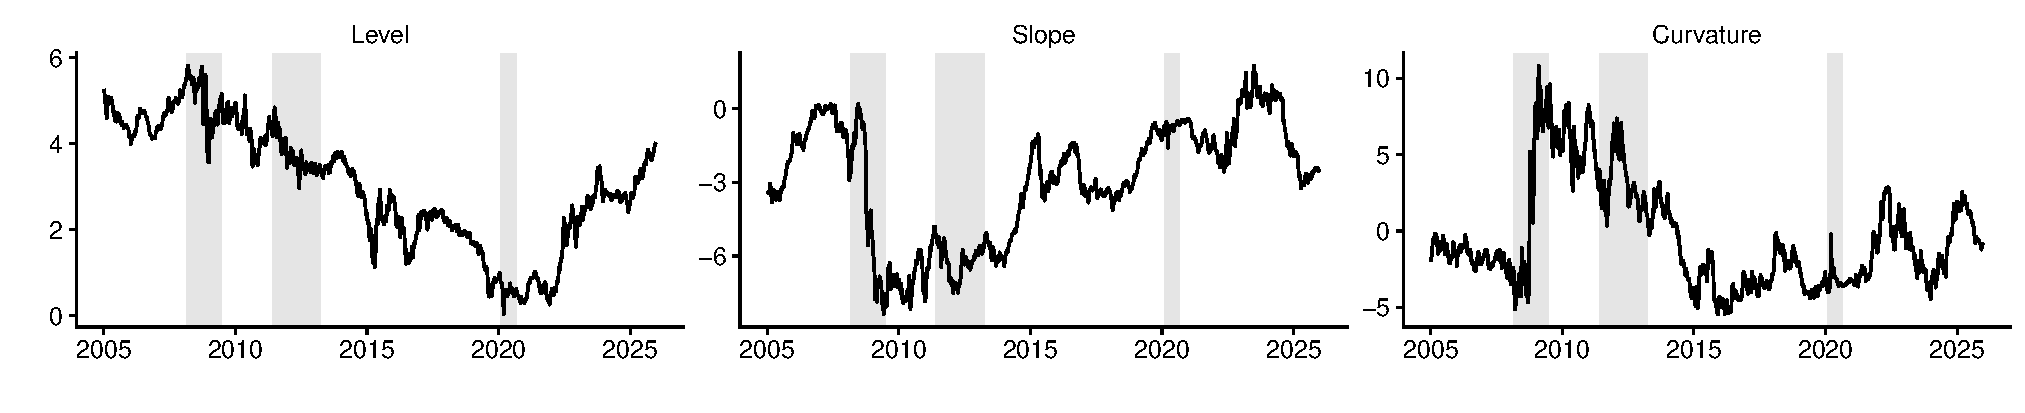
\includegraphics[width=1\textwidth]{images_updated/descript/YLD_NSfacs.pdf}
\end{minipage}
\begin{minipage}{\textwidth}
\centering
\vspace{5pt}
b) Inflation swap curve factors
\end{minipage}
\begin{minipage}{\textwidth}
\centering
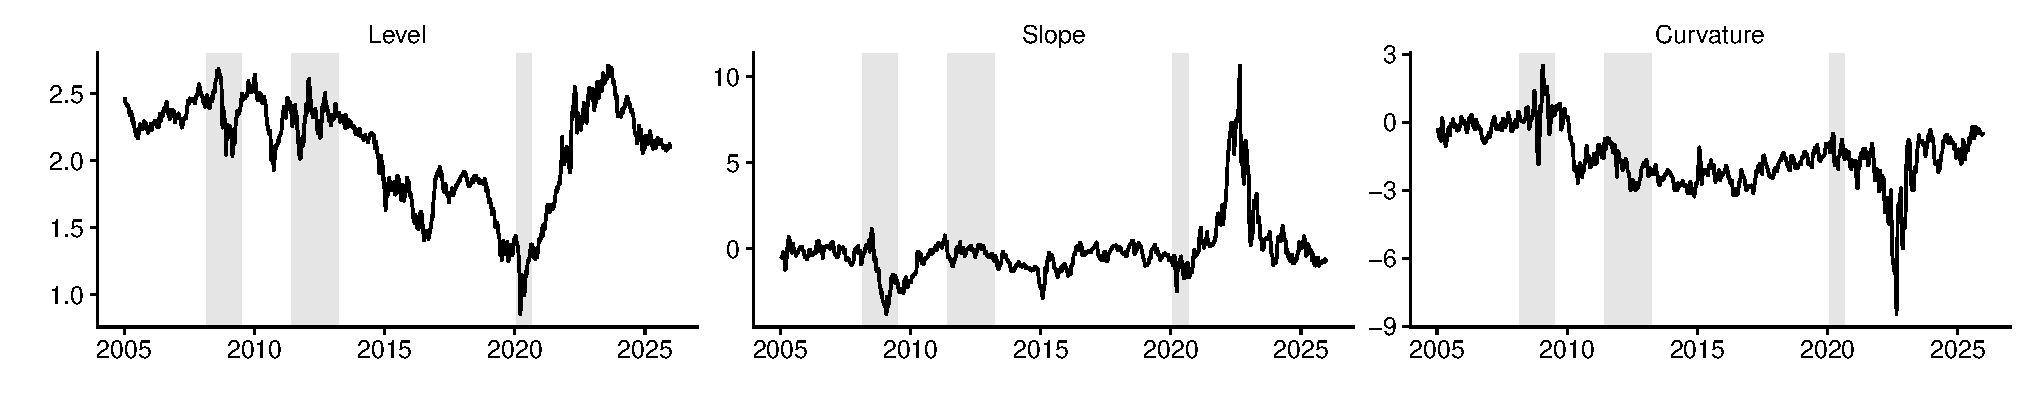
\includegraphics[width=1\textwidth]{images_updated/descript/INFSWP_NSfacs.pdf}
\end{minipage}
\caption*{\textit{Notes:} The factors (shown in levels) are obtained with a three-factor Nelson Siegel model, where $L_{jt}$ can be interpreted as the level, $S_{jt}$ as the slope, and $C_{jt}$ the curvature factor for $j$ being either the associated yield curve ($r$) or the inflation swap curve ($\pi$) factors. Gray shaded areas indicate EA recessions based on the Euro Area Business Cycle Dating Committee. \rev{Factors are shown for the full $2005$--$2025$ sample.}}
\end{figure}

Turning to the estimated factors associated with the inflation swap curve, other interesting findings emerge. First, we find a substantial and persistent decline in the level of inflation expectations \rev{over the first two-thirds of the sample, which subsequently reverses}. Given the level of the yield curve in panel (a) of Fig. \ref{fig:dataNS}, this suggests that real interest rates were positive and then approached negative territory \rev{around 2020. With the post-pandemic inflation surge, however, both nominal yields and inflation swaps rebounded sharply, so that by the end of the sample real interest rates had returned to clearly positive territory}. Both the slope and the curvature of the swap curve show a sharp decline during the global financial crisis. This implies that short-run inflation expectations declined, while long-run inflation expectations either remained constant or increased. Interestingly, a second sharp decline in the slope of the swap curve is observed during the introduction of the Asset Purchase Program (APP) in mid-2014. This and subsequent purchase programs were designed to support the ECB's policy in the face of the effective lower bound. However, \cite{burban2021ILSrisk} provide a decomposition of the ILS into its expectation and risk premium components. Their estimates suggest a change in the sign of the risk premium around 2013/2014. Therefore, this dynamic could also be reflected in our results. After another significant decline in early 2015 to 2016, possibly caused by another round of asset purchases, the slope fluctuates around zero, implying rather stable inflation expectations over different horizons. \rev{This stability breaks down at the end of the extended sample: during 2021--2022 the slope factor of the swap curve spikes sharply, reflecting a pronounced rise in short-horizon relative to long-horizon inflation expectations as headline inflation surged, before receding as the surge faded and expectations re-anchored.} To ensure stationarity, the respective factors are differenced in the estimation.

\subsection{Measuring Monetary Policy}\label{sec:measuring}
In order to detect monetary policy interactions between the US and the euro area, we rely on a unique measure of ECB monetary policy shocks, which renders a separate identification obsolete. Moreover, we use an instrument that is purged of various types of shocks and thus carries only information about monetary policy itself. As shown in \cite{jarocinski2020deconstructing}, central bank communication conveys information not only about monetary policy but also about the state of the economy. This so-called information effect can cause adverse reactions on financial market variables. Therefore, for our purpose of analyzing the effects of monetary policy, we need to make sure that the instruments used are clearly related to monetary policy surprises.
%It is worth mentioning that our  sample covers the zero lower bound episode and thus the implementation of unconventional monetary policy measures. Hence, our surprise series needs to incorporate sufficient information about surprises not stemming from conventional policy actions. Indeed, the choice of the respective monetary policy surprise series may be crucial for the consecutive analysis, such that we provide several robustness checks in \autoref{sec:results_rob}.

A convenient measure of EA monetary policy shocks (i.e., our domestic shocks, $z_{EA,t}$) that satisfies the above requirements has been proposed in \cite{altavilla2019measuring}. This measure is based on the Euro Area Monetary Policy Event-Study Database and exploits the high-frequency reactions of financial markets in a narrow window (ten minutes before and after the event) around identified events associated with monetary policy announcements.\footnote{The full Event-Study Database can be found via \href{https://www.ecb.europa.eu/pub/pdf/annex/Dataset_EA-MPD.xlsx}{https://www.ecb.europa.eu/pub/pdf/annex/Dataset\_EA-MPD.xlsx} and a detailed description of the methodology and data  in \cite{altavilla2019measuring}.} 
The extracted factors consist of the target, the timing, the forward guidance, and the quantitative easing factor, respectively. Each of these factors has an impact on different segments of the yield curve. %Since we are interested in a comprehensive identified measure of monetary policy surprises, we consider a linear combination of these factors.
By taking the sum of these factors, we obtain a broad summary measure of monetary policy surprises.\rev{\footnote{We use the regularly updated factor estimates maintained by Giuseppe Ragusa (\href{https://gragusa.org/factors/}{https://gragusa.org/factors/}, vintage October 2025), which apply the methodology of \cite{altavilla2019measuring} to the current Euro Area Monetary Policy Event-Study Database. Since the factors are re-estimated on the full sample in each vintage, point estimates differ marginally across vintages, with correlations above $0.98$.}} To avoid a contamination of this unified measure with information effects, we use the approach introduced in \cite{jarocinski2020deconstructing}, called "poor-man's sign restrictions". This is achieved by restricting the stock market reaction to policy shocks to be negative in sign. This restriction ensures that we have a measure that only captures monetary policy surprises. \rev{Moreover, \cite{altavilla2019measuring}, Appendix A, flag three announcements (August 31, 2006, October 8, and November 6, 2008) at which no press conference followed the Governing Council meeting, so that the second event window used to identify the timing, forward guidance and quantitative easing factors does not exist. In the vintage we use, two of these dates (October 8 and November 6, 2008) carry no factor values and therefore enter our weekly measure as zeros; the third (August 31, 2006) enters with a surprise of $+2.0$ basis points, negligible against the $5.7$ basis point standard deviation of the series, and we retain it.}

To measure the corresponding US monetary policy stance, denoted $z_t^\ast$, we use the effective federal funds rate, $DFF_t$, and subtract the (one-sided) natural rate estimate, $r^{\ast}$, obtained using the model proposed in \cite{laubach2003measuring}. Since the latter estimate is only available at the quarterly frequency, we use a linear interpolation to adjust it to the weekly frequency. The effective rate thus serves as a fast-moving component of the stance, while the natural rate captures slower trends. This measure allows us to interpret values above (below) zero as a tight (loose) US monetary policy stance. \rev{This constitutes our baseline stance measure. To ensure that our findings do not hinge on how the stance is measured---in particular on the treatment of the effective-lower-bound period, during which the federal funds rate is pinned near zero---we consider two model-based alternatives as robustness checks: the shadow short rate and the effective monetary stimulus of \cite{krippner2016ems}, each taken relative to $r^{\ast}$.}


%For the US monetary policy shocks $z_t^\ast$,  we use the instrument stipulated in \cite{bu2021unified}.We measure the US monetary policy stance through the  unified measure constructed by \cite{bu2021unified}.\footnote{The series can be downloaded via \href{https://www.federalreserve.gov/econres/feds/a-unified-measure-of-fed-monetary-policy-shocks.htm}{https://www.federalreserve.gov/econres/feds/a-unified-measure-of-fed-monetary-policy-shocks.html}.} This constructed shock series conveniently summarizes and quantifies conventional and unconventional monetary policy in the US. While also exploiting variations in a specific time window around FOMC meeting days, the extraction of surprises follows a \cite{famamacbeth1973FedMP} approach and takes periods of conventional and unconventional monetary policy equally into account. The advantages of this measure are twofold. First, the absence of a central bank information effect allows us capturing only the pure monetary policy shocks.  Second, it conveniently pictures US surprises during the zero lower bound episode. 

%For our consecutive analysis, we introduce some persistence to this measure by computing one-quarter ($13$ weeks) moving averages of the instrument. This facilitates interpretation as the Fed's monetary policy stance, since it summarizes unexpected shifts in monetary policy over a longer period of time. This transformed variable then serves as our threshold variable  $z_t^\ast$.  Hence, our measure of the US monetary policy stance is backward looking by about $13$ weeks, implying that shocks occurring in time $t$ impact  the regime allocation for the next $t+13$ periods. %This reflects the notion that monetary policy works with some lags. 

In \autoref{fig:dataMPshk} the monetary policy surprise instruments, $z_{EA,t}$, and the US monetary policy stance, $z_t^\ast$, are shown.\footnote{\rev{Two euro area surprises are exceptional in magnitude and are highlighted with red dots in \autoref{fig:dataMPshk}. We flag them here because both are contaminated by non-monetary-policy events and are therefore excluded, on economic grounds, from all of our estimates --- both the reduced-form pass-through regressions in \autoref{sec:passthrough} and the structural model of \autoref{sec:results}. This exclusion rests on our own judgement about the validity of the surprise and is distinct from the three no-press-conference announcements discussed above, which concern how the factors are constructed rather than how the surprise is interpreted. The first, on 17 March 2023 ($+30.7$ bps), coincides with the collapse of Silicon Valley Bank and the distress at Credit Suisse: the ECB raised rates by 50 basis points into an acute banking-stress episode, yet euro area yields \textit{fell} on a flight to safety, so the co-movement reflects financial-stress dynamics rather than the transmission of the policy surprise itself. The second, on 4 July 2008 ($-23.8$ bps), falls in the week of the ECB's final pre-crisis rate hike at the onset of the global financial turmoil, a period of severe money-market dislocation in which the high-frequency surprise is unusually large and hard to interpret as a clean policy shock. Exclusion is implemented differently in the two settings, for mechanical reasons: the event-week regressions of \autoref{sec:passthrough} drop the two observations from the estimation sample, whereas in the VAR of \autoref{sec:results} the weeks remain in the system and only the surprise itself is set to zero, so that they are treated as weeks without an ECB announcement. Deleting an observation outright is not available in a VAR, where the missing value would propagate through the lag structure and remove several consecutive weeks from every equation. The distinction is immaterial here. With the surprise set to zero, these weeks contribute exactly nothing to the first row and column of the residual covariance matrix, which is what determines the impact responses under our recursive identification; and they are not themselves outliers in the endogenous variables (17 March 2023 moved the ten-year yield by $0.8$ and the two-year yield by $0.1$ standard deviations), together accounting for less than $3\%$ of the residual variation.}} Several features stand out. From the beginning of our sample until the onset of the financial crisis, the Fed pursued a restrictive policy, reflected in a tight stance. To cope with the effects of the crisis, it cut policy rates sharply and introduced additional unconventional measures to counteract the downturn. Most importantly, these measures were designed to support the severely impaired interbank market to maintain liquidity in times of severe financial turmoil and to overcome the constraints imposed by the zero lower bound. The Fed continued its unconventional measures in the form of large-scale bond purchases. As a result, the stance remained rather accommodative until the first quarter of 2017, after which it shifted to a tighter stance given the intention to normalize the balance sheet. \rev{After a renewed easing around the COVID-19 shock, the stance rose sharply during the 2022--2024 tightening cycle, reaching its most restrictive readings of the entire sample.}
The ECB's policy surprises, on the other hand, reveal different information. While the period of the financial crisis was characterized by high upside and downside surprises, in early 2011 the ECB tightened its stance in two consecutive quarters. The benchmark interest rate (on the main refinancing operations) was set at 1.5\% in July, leading to large tightening surprises. Shortly thereafter, the euro area entered a recession, prompting the ECB to adopt a more expansionary policy, with expansionary surprises. In subsequent periods, the surprises have been mixed. \rev{Toward the end of the sample the transatlantic divergence becomes particularly pronounced: the Fed moved to the most restrictive stance of the entire sample during the 2022--2024 tightening cycle, while the euro area monetary policy surprises remained comparatively contained. It is precisely this configuration---a decisively tight Fed outside a euro area recession and away from the effective lower bound---that supplies much of the identifying variation exploited in the state-dependent analysis below.}


%After the financial crisis, in 2010, the euro area headed into a substantial sovereign debt crisis such that  the ECB's policy stance remains quite loose, however with a decreasing pace. In contrast, the Fed continued their bond buying programs at a large scale, represented by a much more pronounced decrease of the surprises. 

%The correlation between the euro area surprises and the Fed policy stance is -0.018 (p-value = 0.61) for the whole sample. 
%However, it might be the case that the correlation is increasing over time, which we check in panel (b) of \autoref{fig:dataMPshk}. Here we plot the rolling correlation between ECB and Fed monetary policy surprises with a one quarter (i.e., 13 weeks) window. The general picture supports the notion of not much coordination between the Atlantic in terms of policy surprises, as only four brief episodes reveal a bit stronger positive correlations, either within recessionary episodes or shortly before/after. This may be explained by the similar required central bank reaction to common shocks hitting both, the euro area and the United States simultaneously.


% \begin{figure}[!htpb]
% \centering
% \caption{Cumulative monetary policy surprises for both EA and US.\label{fig:dataMPshk}}
% 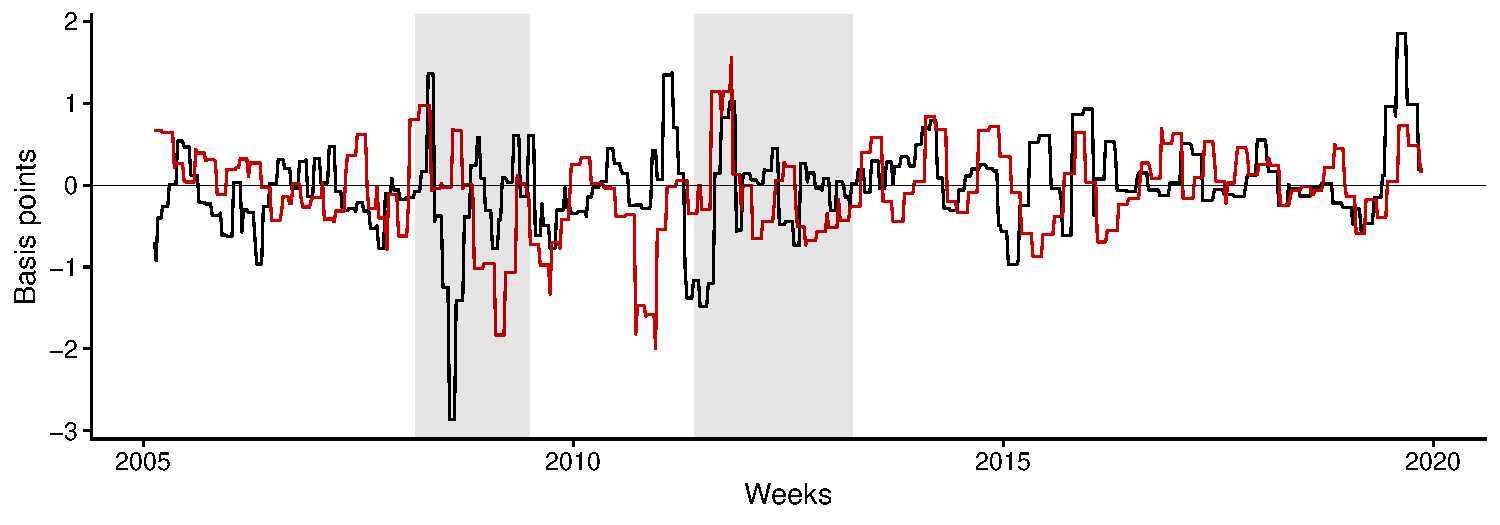
\includegraphics[width=1\textwidth]{images/descript/MPshks_surpr_MA13Motto-Bu.pdf}
% \caption*{\footnotesize \textit{Notes:} The black line denotes cumulative EA monetary policy surprises of \cite{altavilla2019measuring}, while the red line refers to cumulative US monetary policy surprises of \cite{bu2021unified} in basis points. Gray shaded areas indicate EA recessions based on the the Euro Area Business Cycle Dating Committee.}
% \end{figure}

\begin{figure}[htpb!]
\centering
\caption{EA Monetary policy surprises (black) and US monetary policy stance (\rev{blue}). \label{fig:dataMPshk}}
%\begin{minipage}{\textwidth}
%\centering
%a) Surprises smoothed with MA(13)
%\end{minipage}
%\begin{minipage}{\textwidth}
\centering
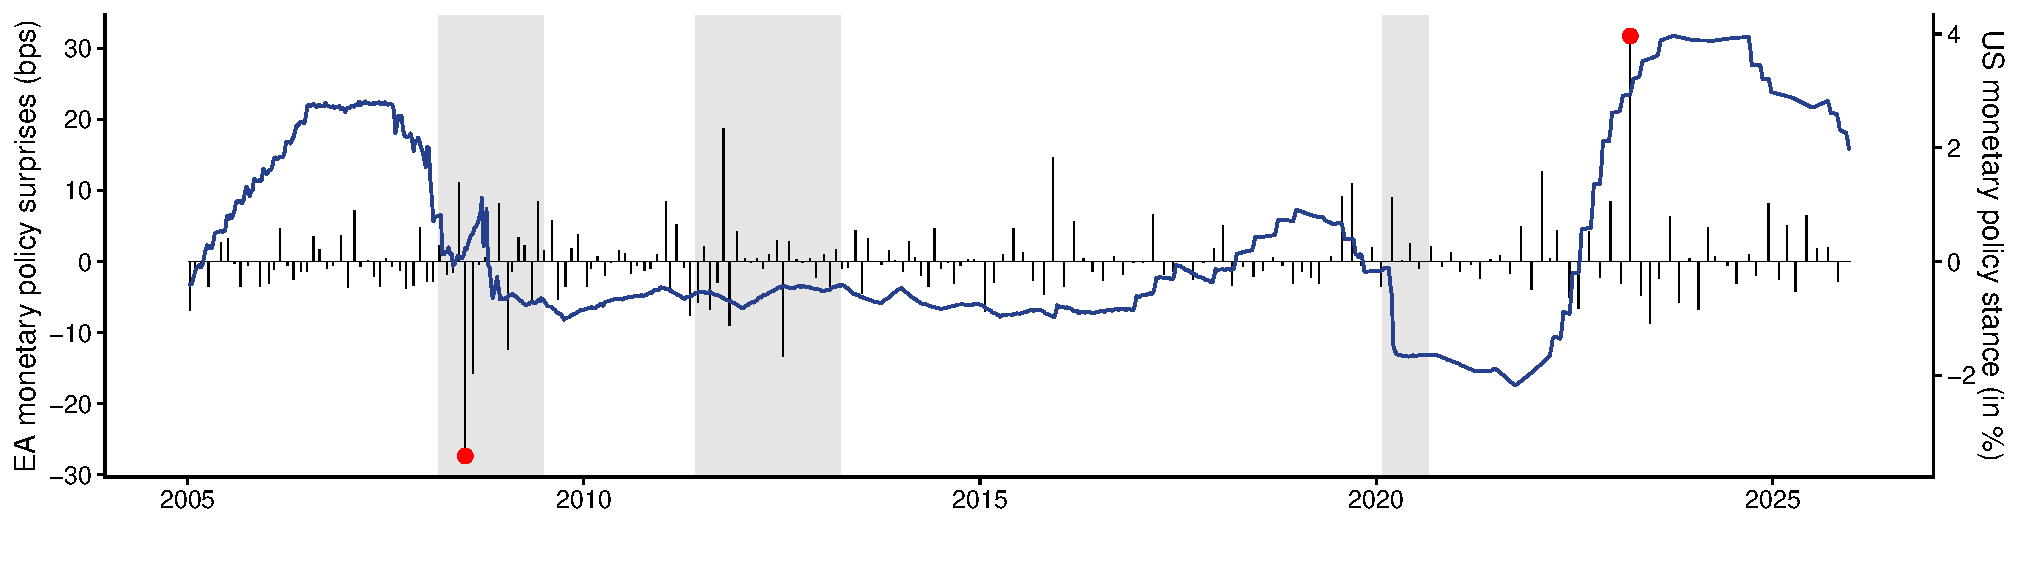
\includegraphics[width=1\textwidth]{images_updated/descript/MPshks_surpr_US_stance.pdf}
% \end{minipage}
% \begin{minipage}{\textwidth}
% \centering
% \vspace{5pt}
% b) Rolling correlation with one quarter (13 weeks) window between EA and US surprises
% \end{minipage}
% \begin{minipage}{\textwidth}
% \centering
% 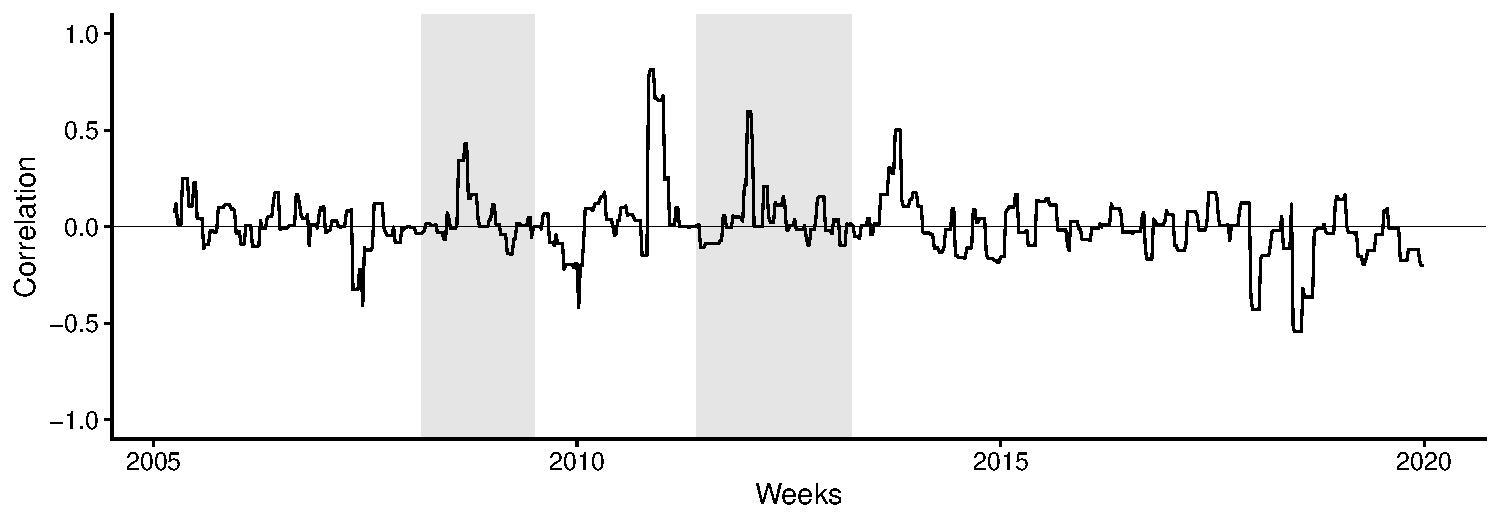
\includegraphics[width=1\textwidth]{images/descript/MPshks_surpr_MA13_rollcorrMotto-Bu.pdf}
% \end{minipage}
\caption*{\textit{Notes:} The black bars denote the EA monetary policy surprises of \cite{altavilla2019measuring}, while the \rev{blue} line refers to the US monetary policy stance ($DFF_t-r^{\ast}$). Gray shaded areas indicate EA recessions based on the Euro Area Business Cycle Dating Committee. \rev{The two red dots mark the two outlier surprises discussed in the text (17 March 2023 and 4 July 2008). Shown for the full $2005$--$2025$ sample.}}
\end{figure}




\subsection{\rev{Transmission of ECB surprises across the term structure}}\label{sec:passthrough}

\rev{Before turning to the dynamic model, we establish how euro area financial markets respond to an ECB monetary policy surprise, and we use the exercise to frame the central question of the paper. For each maturity $\tau$ we regress the weekly change in the nominal yield, and separately in the inflation-linked swap rate, on the euro area surprise,}
\begin{equation}\label{eq:passthrough}
    {\color{red} \Delta y^{\tau}_{t} = a_{\tau} + b_{\tau}\,\mathrm{MP.EA}_t + \varepsilon^{\tau}_{t},}
\end{equation}
\rev{and trace the estimated pass-through coefficient $b_{\tau}$ along the whole term structure. \autoref{fig:passthrough} plots $b_{\tau}$ (in basis points of yield per basis point of surprise) for all $15$ maturities, with $90\%$ confidence bands. Two ECB surprises are extreme outliers contaminated by contemporaneous financial-stress events; they are excluded from the baseline on economic grounds (see the discussion around \autoref{fig:dataMPshk}), and the dashed line shows that including them attenuates the estimates but leaves the maturity profile unchanged.}
\begin{figure}[ht!]
\centering
\caption{\rev{Pass-through of ECB monetary policy surprises along the term structure.}}\label{fig:passthrough}
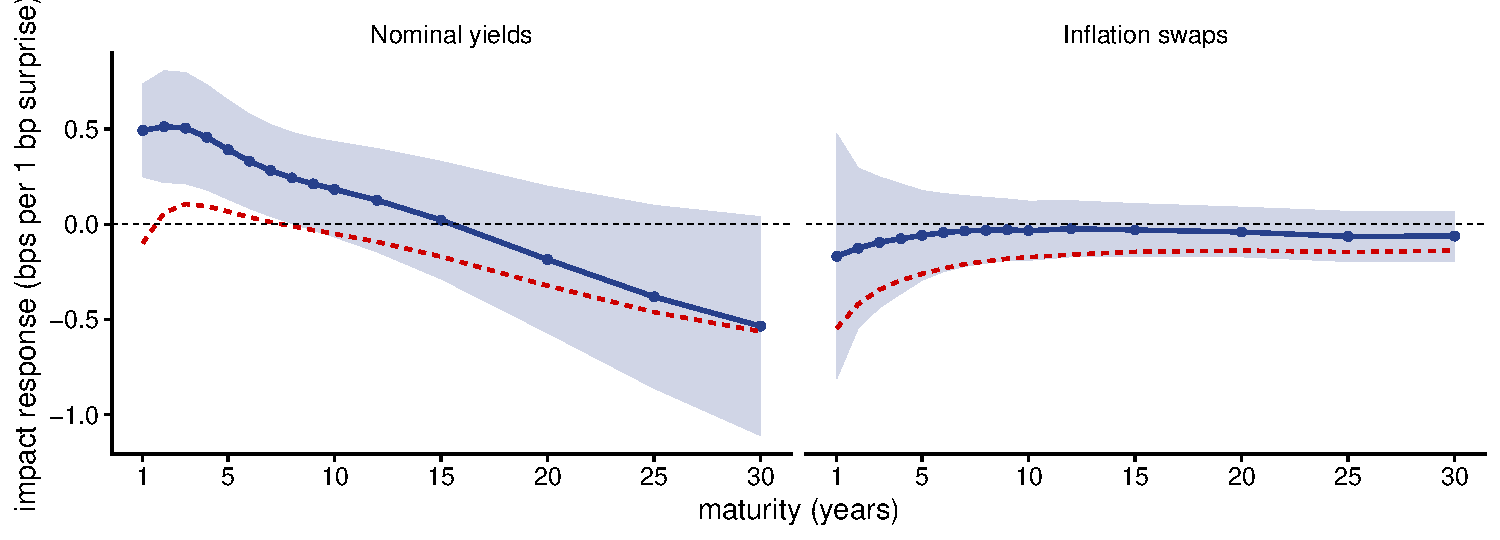
\includegraphics[width=\textwidth]{images_updated/passthrough_curve.pdf}
\caption*{\rev{\footnotesize \textit{Notes:} Each point is the slope coefficient $b_\tau$ from an event-week regression \eqref{eq:passthrough} of the weekly change in the nominal yield (left) or inflation-linked swap (right) of maturity $\tau$ on the euro area monetary policy surprise \citep{altavilla2019measuring}, expressed in basis points of yield per basis point of surprise. The solid line and shaded $90\%$ band exclude the two outlier surprises discussed in \autoref{sec:measuring} (17 March 2023 and 4 July 2008); the red dashed line includes all events. Heteroskedasticity-consistent standard errors; weekly data, 2005--2025.}}
\vspace{-3mm}
\end{figure}
\rev{Three features stand out. First, the surprise transmits strongly to \textit{nominal} yields at the short end: a one-basis-point tightening surprise raises the one- to three-year yield by about half a basis point ($t\approx 3$), an effect that declines monotonically with maturity and is indistinguishable from zero beyond ten years. Second, the response of inflation-linked swaps is negative but small and imprecisely estimated at all maturities, so the tightening is transmitted primarily to \textit{real} rates: the implied short-maturity real yield rises by roughly one-half to two-thirds of a basis point per basis point of surprise ($t\approx 2$). Third, the pattern is a genuine term-structure phenomenon --- transmission is concentrated at the maturities where conventional and forward-guidance policy operate and dissipates at longer horizons. Taken together, these facts confirm that our instrument captures economically meaningful, correctly signed monetary policy surprises, and they put to work the full yield and inflation-swap curves that are the empirical contribution of this paper.}

\rev{The question this paper is concerned with is whether this transmission depends on the stance of US monetary policy. Simple, model-free tools cannot answer it. Splitting the sample into loose- and tight-Fed weeks and running \eqref{eq:passthrough} separately, or estimating state-dependent local projections out to a quarter, yields loose- and tight-regime responses that are statistically indistinguishable at weekly frequency, and the little contrast that does appear is sensitive to individual high-leverage observations.\footnote{\rev{Across maturities and horizons the loose-versus-tight difference in the impact response is statistically insignificant, with $p$-values above $0.5$ once the two outlier surprises discussed in \autoref{sec:measuring} are excluded. These checks are available upon request.}} This is unsurprising: weekly financial data have a low signal-to-noise ratio, the exercise ignores dynamics, and a binary split coarsely discretizes a continuous stance. Answering the question convincingly requires a framework that pools information across the whole system, replaces the binary split with a smooth transition in the Fed's stance, allows for dynamics beyond the impact week, and disciplines the resulting parameter proliferation through shrinkage. This is precisely the smooth-transition VAR to which we now turn.}

%%% [REVISION 2026-07] The previous motivating exercise --- a scatter of first-differenced real 10-year
%%% yields split by the Fed stance (former Figure "fig:interaction", images/new_Regression_plot.pdf) and
%%% the accompanying Nelson-Siegel interaction regression (former Table "tab:regression") --- has been
%%% REPLACED by the term-structure pass-through analysis above. On the 2005-2025 sample the earlier
%%% sign-switch was not robust: it was driven by two outlier surprises (above all the SVB / Credit Suisse
%%% week of 17 March 2023). The retired equation, table and discussion are preserved but not typeset,
%%% inside the \iffalse ... \fi block below.
\iffalse

%As we showed in \autoref{fig:interaction} in the introductory section, there exists a considerably different effect of monetary policy shocks on the euro area 10-year real bond yields if we account for the respective Fed's policy stance. 

%After obtaining the \textit{full} yield and inflation expectation term structure by employing the constructed Nelson-Siegel factors of the respective curve (see \autoref{fig:dataNS}), we are able to take a closer look at which factors are affected most by interaction effects. In \autoref{tab:regression} we report the results of regressing the obtained yield and swap curve factors on the ECB's policy surprises  and the changes in the Fed's stance, as well as on the interaction between those instruments.

Specifically, we use our  constructed Nelson-Siegel factors of the nominal yield and inflation swap curve (see \autoref{fig:dataNS}) and estimate 
\begin{equation}\label{eq:univRegr}
    y_{it} = \beta_{i0} + \beta_{i1}\text{MP.EA}_t + \beta_{i2}\Delta\text{MP.US}_t + \gamma_{i} (\text{MP.EA}_t \times \Delta\text{MP.US}_t) + \epsilon_{it}
\end{equation}
where $i\in\{L, S, C\}$ denotes the level, slope, and curvature factor of the yields and swaps in their level values, MP.EA is the EA monetary instruments used, $\Delta$MP.US is the change in the Fed's policy stance, and $\epsilon_{it}$ is an error term. The interaction effect $\text{MP.EA}_t \times \Delta\text{MP.US}_t$ is quantified by the coefficient $\gamma$. We report the results of this exercise in \autoref{tab:regression}.  %This regression measures the contemporaneous effect of the ECB's monetary policy on the key factors driving the yield curve, controlling for nonlinearities caused by the US monetary policy stance. %\textbf{We might want to draw the connection to LPs which would arise if we have $y_{it+h}$ for $h=0, ..$ as dependent variable.}

\begin{table}[!htbp]\centering 
  \caption{Yield and inflation swap curve factors and monetary policy interactions} 
  \label{tab:regression} 
\begin{tabular}{@{\extracolsep{5pt}}lcccccc} 
\\[-1.8ex]\hline 
\hline \\[-1.8ex] 
 & \multicolumn{6}{c}{\textit{Dependent variable:}} \\ 
\cline{2-7} 
\\[-1.8ex] & \multicolumn{3}{c}{Yield Curve factor} & \multicolumn{3}{c}{Inflation Swap Factor} \\ 
\\[-1.8ex] & $L_r$ & $S_r$ & $C_r$ & $L_{\pi}$ & $S_{\pi}$ & $C_{\pi}$\\ 
\hline \\[-1.8ex]
 \color{red} Constant & \color{red} 3.043$^{***}$ & \color{red} $-$3.371$^{***}$ & \color{red} $-$0.397$^{***}$ & \color{red} 2.041$^{***}$ & \color{red} $-$0.385$^{***}$ & \color{red} $-$1.447$^{***}$ \\
  & \color{red} (0.051) & \color{red} (0.079) & \color{red} (0.123) & \color{red} (0.013) & \color{red} (0.040) & \color{red} (0.037) \\
  & & & & & & \\
 \color{red} MP.EA & \color{red} $-$0.050$^{**}$ & \color{red} $-$0.008 & \color{red} 0.034 & \color{red} $-$0.012$^{**}$ & \color{red} 0.014 & \color{red} $-$0.024 \\
  & \color{red} (0.025) & \color{red} (0.039) & \color{red} (0.066) & \color{red} (0.006) & \color{red} (0.022) & \color{red} (0.019) \\
  & & & & & & \\
 \color{red} $\Delta$MP.US & \color{red} $-$0.052 & \color{red} $-$0.782 & \color{red} 0.811 & \color{red} 0.302 & \color{red} 2.082$^{***}$ & \color{red} $-$1.170$^{**}$ \\
  & \color{red} (0.874) & \color{red} (0.675) & \color{red} (1.396) & \color{red} (0.236) & \color{red} (0.596) & \color{red} (0.528) \\
  & & & & & & \\
 \color{red} MP.EA$\times$$\Delta$MP.US & \color{red} $-$0.147 & \color{red} $-$0.559 & \color{red} $-$0.374 & \color{red} 0.023 & \color{red} 0.147 & \color{red} $-$0.436$^{**}$ \\
  & \color{red} (0.365) & \color{red} (0.386) & \color{red} (0.701) & \color{red} (0.101) & \color{red} (0.374) & \color{red} (0.173) \\
  & & & & & & \\
\hline \\[-1.8ex]
\color{red} Observations & \color{red} 899 & \color{red} 899 & \color{red} 899 & \color{red} 899 & \color{red} 899 & \color{red} 899 \\
\color{red} R$^{2}$ & \color{red} 0.005 & \color{red} 0.002 & \color{red} 0.001 & \color{red} 0.009 & \color{red} 0.021 & \color{red} 0.013 \\
\hline
\hline \\[-1.8ex]
\end{tabular}
{\parbox{0.9\textwidth}{\textit{Notes:} Ordinary least squares regression of the respective Nelson-Siegel factor on a constant, the monetary policy surprises  for the euro area (MP.EA), the first differences of the US monetary policy stance ($\Delta$MP.US) and the interaction effect with the EA surprises (MP.EA$\times$$\Delta$MP.US). Heteroskedasticity-consistent standard errors are reported in parentheses, $^{*}$, $^{**}$ and $^{***}$ denote significance on the 10\%, 5\% and 1\% level. \rev{Estimates are based on the updated data vintage described in \autoref{app:0} (revised natural rate estimates and re-estimated policy surprise factors) over the 2005--2022 sample, since the dependent variables involve the inflation-swap curve, which ends in May 2022.}}}
\end{table} 



%The interpretation of the magnitude of the coefficients is not straightforward as we have to map them back via the Nelson-Siegel decomposition. %As the simple regression analysis should just serve as further motivation for the larger model, we do not provide an extensive analysis here.


% \begin{table}[!htbp] \centering 
% \caption{Yield curve factors and monetary policy interactions} \label{tab:IE_yields}
% \begin{tabular}{@{\extracolsep{5pt}}lccc} 
% \hline \\[-1.8ex] 
%  & \multicolumn{3}{c}{\textit{Yield curve factor:}} \\ 
% \cline{2-4} 
% \\[-1.8ex] & Level & Slope & Curvature\\ 
% \hline \\[-1.8ex] 
%  Constant & $-$0.006 & 0.005 & $-$0.004 \\ 
%   & (0.005) & (0.008) & (0.021) \\ 
%   & & & \\ 
%  MP.EA & $-$0.001 & 0.013$^{***}$ & 0.013 \\ 
%   & (0.002) & (0.003) & (0.009) \\ 
%   & & & \\ 
%  MP.US & $-$0.006 & 0.018 & $-$0.002 \\ 
%   & (0.009) & (0.015) & (0.039) \\ 
%   & & & \\ 
%  MP.EA:MP.US & 0.004 & $-$0.019$^{***}$ & 0.009 \\ 
%   & (0.003) & (0.005) & (0.015) \\ 
%   & & & \\ 
% \hline \\[-1.8ex] 
% Observations & 774 & 774 & 774 \\ 
% R$^{2}$ & 0.003 & 0.032 & 0.004 \\ 
% Residual Std. Error (df = 770) & 0.131 & 0.213 & 0.574 \\ 
% \hline 
% \hline \\[-1.8ex] 
% \end{tabular} 
% {\parbox{0.9\textwidth}{\textit{Notes:} Ordinary least squares regression of the respective Nelson-Siegel factor on a constant, the monetary policy instruments  for the euro area (MP.EA), the US (MP.US) and the interaction effect of both instruments (MP.EA:MP.US). Standard errors in parentheses. $^{*}$, $^{**}$ and $^{***}$ denote significance on the 10\%, 5\% and 1\% level.}}
% \end{table} 

\rev{We observe that the constant is highly significant in all specifications, while euro area policy surprises on their own have at most a marginal effect on the factors. The interaction terms carry a uniformly negative sign for the yield curve factors and are statistically significant for the curvature of the swap curve, while a tightening of the US stance is associated with a steepening of the swap curve. The precision of these unconditional least squares estimates is limited --- unsurprisingly so, given the low signal-to-noise ratio of weekly financial data and the absence of any dynamics in this specification. We therefore regard this exercise as merely suggestive: it hints at a state-dependent transmission working through the term structure, but quantifying it requires the dynamic multivariate framework to which we now turn.}


%a restrictive stance in general has a decreasing effect on the typically ascending yield curve. However, this changes if we take the interaction effect into account. The marginal effect of an ECB policy surprise on the yield curve slope seems to be offset if the Fed also tightens its stance. Put differently, the effectiveness of the ECB's policy is crucially intercepted by its US counterpart when it comes to the slope of the yield curve. Based on this simple exercise, we may conclude that the Fed's surprises crucially impede the euro area monetary policy transmission channels that affect the yield curve.While the level of the inflation swap curve decreases after a tightening surprise, the effect is rather negligible and not significant. However, if the Fed contemporaneously tightens as well, the level factor compression is much more pronounced. This points towards  US disinflation dynamics that amplify the domestic effect of monetary policy. From the slope factor reactions, we conclude that the interaction effect points towards a steepening effect on the swap curve. 

\fi
%%% [end of retired motivating-regression block]

%While this simplistic specification provides only a contemporaneous picture, the change of the sign of the relationship, i.e., the way ECB monetary policy effects real bond yields \textit{conditional} on the Fed's stance is remarkably and warrants a more holistic empirical analysis. This state-dependent reaction of bond yields to ECB monetary policy suggests that the Fed's current stance needs to be taken into account for adequately assessing the effects of the ECB's monetary policy.

%An example is the omission of effects that simultaneously alter the shape of the yield and swap curves. Moreover, a contemporaneous reaction of yields and inflation swaps might be likely and potentially exhibits offsetting dynamics. To gain a deeper understanding,  we will thus  provide evidence based on our ST-VAR  in the subsequent sections.

%We repeat this exercise in \autoref{eq:univRegr} with the corresponding inflation swap factors and report the results in \autoref{tab:IE_swaps}.  Compared to the yield curve factors, we observe a statistically significant reaction due to ECB surprises only for the slope factor and  the monetary policy interaction part only for the level. That is, the respective level of inflation expectations decreases after the Fed produces a positive surprise, though the effect is rather negligible. This points towards imported disinflation dynamics from the US that amplify the domestic effect of monetary policy. Given the results from the curvature part of the expectation term structure, we neither see pronounced reactions to ECB surprises nor substantial interaction effects. While this univariate analysis suffers from several shortcomings (such as the low explanatory power and the focus on contemporaneous relations between yield curve dynamics and monetary policy) and thus serves only as a motivation for a unified analysis, it motivates further explorations. An example is the omission of effects that simultaneously alter the shape of the yield and swap curves. Moreover, a contemporaneous reaction of yields and inflation swaps might be likely and potentially exhibits offsetting dynamics. To gain a deeper understanding,  we will thus  provide evidence based on our ST-VAR  in the subsequent sections.


% \begin{table}[!htbp] \centering 
%   \caption{Inflation swap factors and monetary policy interactions} \label{tab:IE_swaps}
% \begin{tabular}{@{\extracolsep{5pt}}lccc} 
% \hline \\[-1.8ex] 
%  & \multicolumn{3}{c}{\textit{Inflation swap factor:}} \\ 
% \cline{2-4} 
% \\[-1.8ex] & Level & Slope & Curvature\\ 
% \hline \\[-1.8ex] 
%  Constant & $-$0.001 & 0.001 & $-$0.002 \\ 
%   & (0.001) & (0.006) & (0.007) \\ 
%   & & & \\ 
%  MP.EA & 0.001 & 0.006$^{**}$ & 0.003 \\ 
%   & (0.001) & (0.003) & (0.003) \\ 
%   & & & \\ 
%  MP.US & $-$0.002 & 0.001 & $-$0.007 \\ 
%   & (0.003) & (0.012) & (0.013) \\ 
%   & & & \\ 
%  MP.EA:MP.US & $-$0.002$^{**}$ & $-$0.006 & $-$0.003 \\ 
%   & (0.001) & (0.004) & (0.005) \\ 
%   & & & \\ 
% \hline \\[-1.8ex] 
% Observations & 774 & 774 & 774 \\ 
% R$^{2}$ & 0.008 & 0.008 & 0.002 \\ 
% Residual Std. Error (df = 770) & 0.037 & 0.170 & 0.191 \\ 
% \hline 
% \hline \\[-1.8ex] 
% \end{tabular} 
% {\parbox{0.9\textwidth}{\textit{Notes:} Ordinary least squares regression of the respective Nelson-Siegel factor on a constant, the monetary policy instruments  for the euro area (MP.EA), the US (MP.US) and the interaction effect of both instruments (MP.EA:MP.US). Standard errors in parentheses. $^{*}$, $^{**}$ and $^{***}$ denote significance on the 10\%, 5\% and 1\% level.}}
% \end{table} 


 
 
\subsection{Monetary Policy Regimes}\label{sec:regimes}
According to our specification in \autoref{eq:STVAR}, the interaction between the US monetary policy stance and the coefficients of our VAR system is encoded by the function $g$ in \autoref{eq:St}. An important intermediate result is thus reported in \autoref{fig:stallo}, showing the posterior mean of $S_t$ (gray area, left scale) \rev{together with its 68\% posterior credible band} alongside the threshold variable over time (red line, right scale). Thus, it provides information about how $S_t=g(z_t^*)$ evolves over time. In principle, values of $S_t$ close to zero indicate periods characterized by a predominantly expansionary (i.e., negative) Fed stance, while values close to unity indicate periods characterized by a restrictive (i.e., positive) Fed stance. \rev{Since the threshold is calibrated at the neutral stance (see \autoref{sec:framework}), the mapping is direct: $S_t$ exceeds $0.5$ exactly when the federal funds rate is above the natural rate (dotted line), and the remaining posterior uncertainty---stemming from the transition speed $\rho$---is visibly small. As the Fed's 2004--2006 hiking cycle pushed the policy rate above the natural rate in early 2005, $S_t$ rises quickly and stays close to unity throughout 2006--2007, indicating that the corresponding VAR coefficients were close to $\bm A_{1j}$. During the financial crisis, the Fed lowered its policy rate rapidly and introduced unconventional monetary policy measures to overcome the restrictions of the zero lower bound: $S_t$ declines through 2008 and reaches low values by early 2009. Throughout the subsequent zero-lower-bound decade the allocation remains clearly expansionary, with $S_t$ fluctuating between roughly $0.1$ and $0.25$ rather than collapsing to zero---the stance was persistently below neutral, but its distance from neutral varied with the evolution of the natural rate.}

%three more pronounced expansionary periods with $S_t \approx 0$. The first can be found in late 2010 and the second is located in the second half of 2012. These two periods are characterized by the introduction of the second and third installment of the quantitative easing program of the Fed. Moreover, it is worth noting that in 2011 the Fed implemented the "Operation Twist", which essentially put downward pressure on longer-term bond yields, while maintaining the short maturity rates at the same level, ultimately leading to a twisted yield curve. This additionally explains the strong expansionary period around 2011 in \autoref{fig:dataMPshk}. The last expansionary period in our sample is July 2019, where the Fed again reduced the rate by 0.25 percentage points. In general, our results square with detailed analyses of US monetary policy and its implemented measures, like, for instance, in \cite{chen2016FedPolicy}.
\begin{figure}[!htpb]
\centering
\caption{State allocation for the EA with the US monetary policy stance as threshold variable. \rev{[Updated: full sample 2005--2025.]}}\label{fig:stallo}
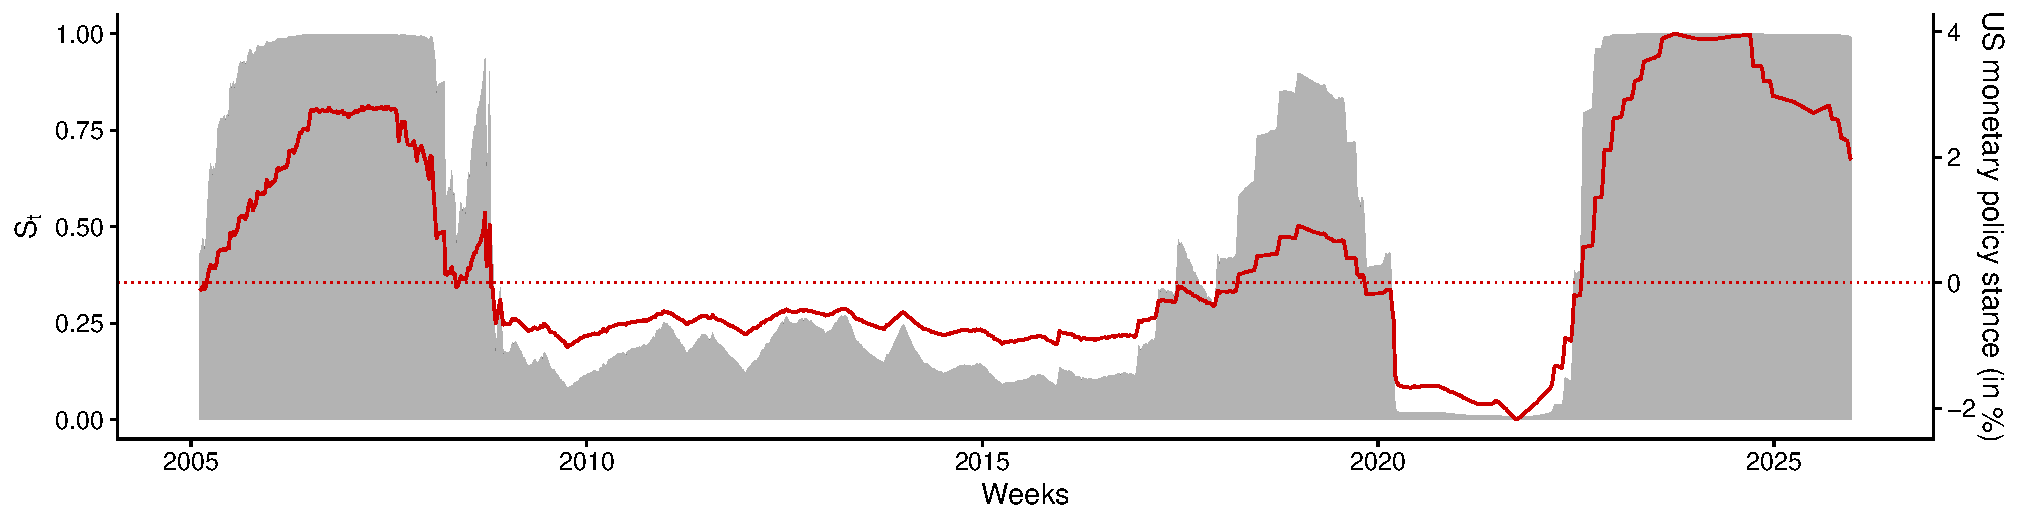
\includegraphics[width= 1\textwidth]{images_updated/DIFF_EA_Motto/St.pdf}
\caption*{\footnotesize \textit{Notes:} Gray areas denote the posterior mean of $S_t$, the transition function, where 0 (1) indicates an expansive (restrictive) regime\rev{; the darker shading marks the 68\% posterior credible band}. The red line depicts the constructed US monetary policy indicator in percent, as defined in \autoref{sec:measuring}\rev{, with the dotted line marking the neutral stance (zero), at which the calibrated transition function crosses $S_t = 0.5$. Estimated on the full 2005--2025 sample (specification \texttt{main} in the replication code \texttt{Codes/STVARestimation.R}); the swap-augmented system covers the entire sample thanks to the 2026 ILS data update. The state allocation is invariant to the outlier exclusion described in \autoref{sec:measuring}, since it depends only on the US stance and the calibrated transition parameters.}}\end{figure}
Given the gradual improvement in US economic conditions from 2013, the Fed began to scale back some of the expansionary measures, most notably through the tapering of the third large-scale asset purchase program, which began in January and ended in October 2014. The Fed's balance sheet remained at the same level until the fall of 2017, when the Fed began a slow unwinding. In addition, the December 2015 FOMC meeting marked a period where the Fed decided to gradually raise interest rates. This led to a gradual tightening with one hike in 2016, three hikes in 2017, and four hikes in 2018, each by 25 basis points. \rev{This hiking cycle lifts the policy rate above the natural rate in the spring of 2018, and $S_t$ accordingly moves into restrictive territory (annual averages of about $0.7$ in 2018--2019)---a mildly restrictive interlude that ends when the Fed's insurance cuts push the stance back below neutral in late 2019. The model then places the COVID-19 episode firmly in the expansionary regime, with $S_t$ falling essentially to zero in 2021. The most informative episode for our purposes, however, is the most recent one: in response to the post-pandemic inflation surge the Fed tightened sharply, the stance crosses neutral in mid-2022, and $S_t$ remains pinned at unity from 2023 through the end of 2025, mirroring---and in both magnitude and duration exceeding---the restrictive phase of 2006--2007. This is the first pronounced restrictive-Fed episode in our sample that occurs outside a recession and away from the effective lower bound, and it is precisely this variation that sharpens the identification of the state-dependent responses discussed below. Equipped with this information, we now proceed with the dynamic analysis.}



\section{Dynamic Responses to a Monetary Policy Shock in the Euro Area}\label{sec:results}
In this section, we discuss the responses to a restrictive monetary policy shock in the euro area. These responses are computed while explicitly conditioning on the US monetary policy stance. This exercise allows us to answer the question of how the monetary policy effect might change in the face of a divergent Fed policy. We therefore report and analyze impulse response functions (IRFs) based on our framework outlined in detail in \autoref{sec:framework}. 

Given our setup, we are able to trace how the transmission of ECB policy shocks varies with the \textit{entire} range of the Fed's stance. The transition function $g(z^\ast_t)$ delivers a distinct set of dynamic coefficients for every value of the Fed's stance, such that we have continuous mapping from the stance to the response of each variable. We therefore start with the continuum of responses in \autoref{fig:headline} for the one-week-ahead reaction of nominal government bond yields (top row), inflation swaps (middle row), and real yields (bottom row) at four selected maturities, plotting the response against the percentile of the Fed's stance. Reading the figure row-wise delivers our central result together with its economic decomposition.

\begin{figure}[!htpb]
\centering
\caption{One-week-ahead response of EA nominal yields, inflation swaps, and real yields to a restrictive ECB surprise, as a function of the Fed's monetary policy stance.}\label{fig:headline}
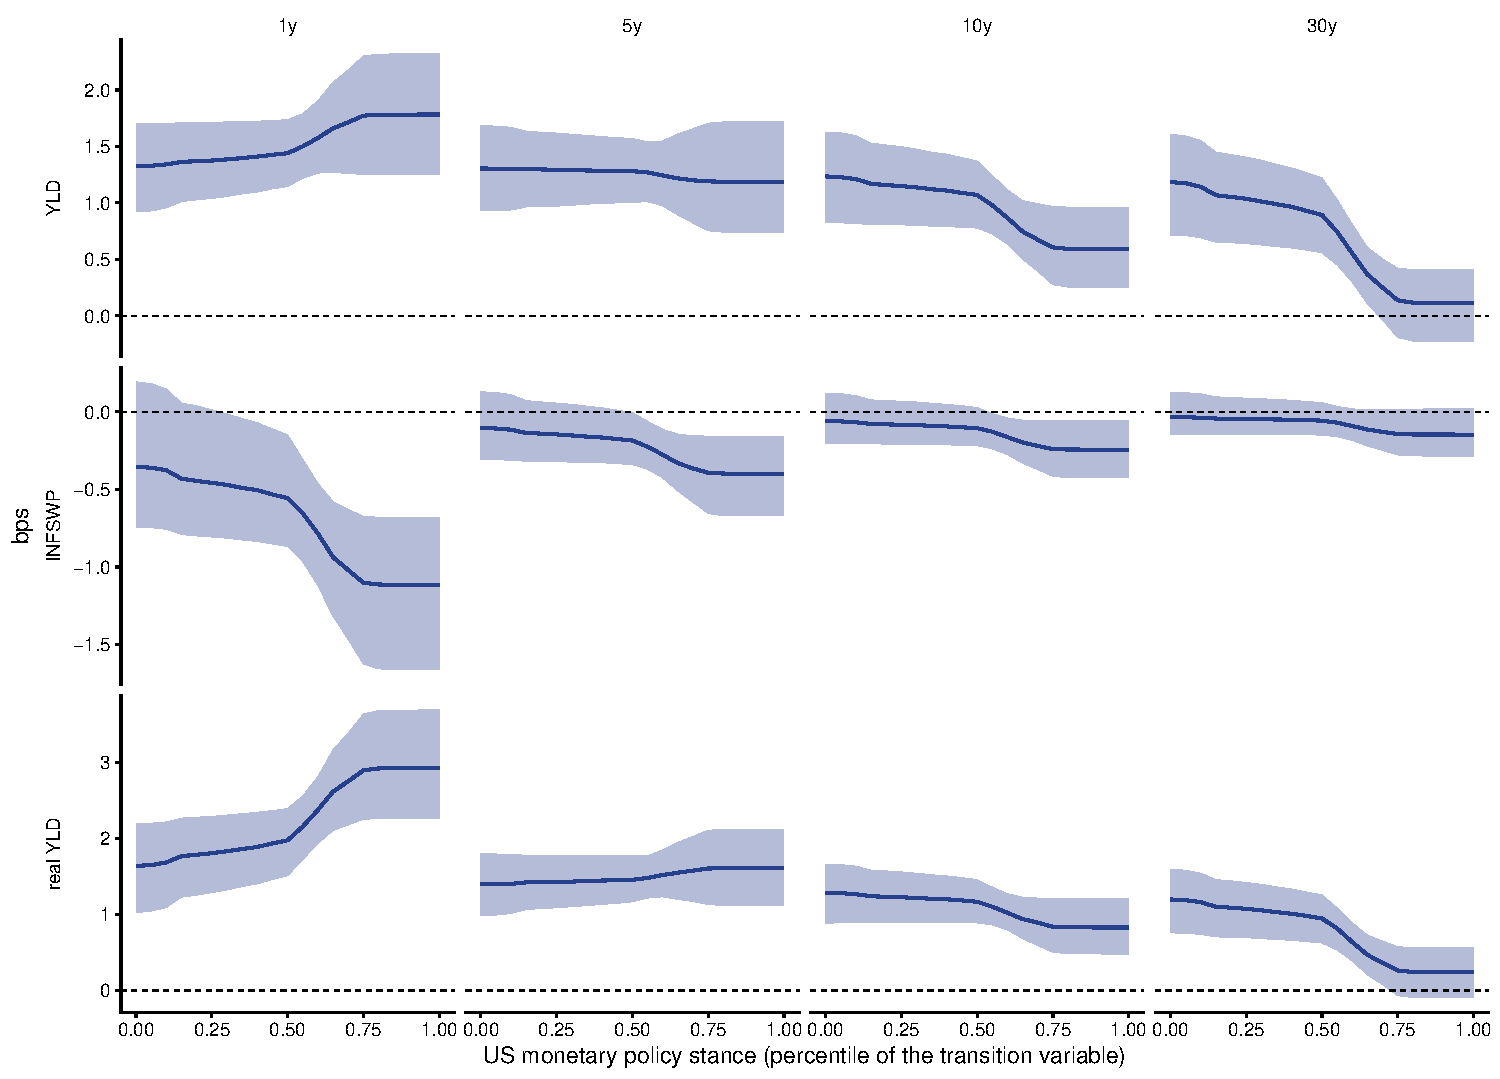
\includegraphics[width=\textwidth]{images_updated/rev/IRF_continuum_panel3.pdf}
\caption*{\footnotesize \textit{Notes:} Posterior median (solid) and $68\%$ credible set (shaded) of the one-week-ahead ($h=1$) response of the indicated variable to a one-standard-deviation restrictive ECB surprise, plotted against the percentile of the US monetary policy stance $z^\ast_t$ (0 = most accommodative, 1 = most restrictive). Rows: nominal government bond yields (YLD), inflation-linked swaps (INFSWP), and real yields (real YLD), where the real-yield response is computed draw-wise as the nominal minus the swap response. Columns: maturities of 1, 5, 10, and 30 years. Responses are in basis points.}
\end{figure}

%The central object of interest is how the transmission of an ECB surprise varies with the \textit{entire} range of the Fed's stance, not merely at two extremes. We therefore lead with the continuum of responses: because the transition function $g(z^\ast_t)$ delivers a distinct set of dynamic coefficients for every value of the Fed's stance, our model traces out a continuous mapping from the stance to the response of each variable. \autoref{fig:headline} presents this mapping for the one-week-ahead reaction of nominal government bond yields (top row), inflation swaps (middle row), and real yields (bottom row) at four selected maturities over the full 2005--2025 sample, plotting the response against the percentile of the Fed's stance. Reading the figure row-wise delivers the paper's central result together with its economic decomposition; note that, draw by draw, the nominal response equals the real response plus the response of inflation compensation.

The headline finding is that the Fed's stance does not shift the pass-through of ECB surprises up or down: it \textit{rotates} it. When the Fed is accommodative, a restrictive ECB surprise raises nominal yields by a similar amount along the whole curve, from $1.3$ basis points at one year to $1.2$ at thirty. When the Fed is restrictive (ninety-fifth percentile), the same surprise raises the one-year yield by more ($1.8$ basis points) but the reaction then falls monotonically with maturity, to $1.2$ basis points at five years, $0.6$ at ten, and $0.1$ at thirty, where it can no longer be distinguished from zero. The two profiles cross between three and five years. Thus, the state dependence is absent at the short end, where the accommodative response falls short of the restrictive one and becomes both sizeable and well determined at the long end. The state dependence of ECB transmission is thus a phenomenon of the \textit{long} end of the curve.

This maturity pattern is thus not uniform. Short-dated yields are governed by the expected path of the ECB's own policy rate, which responds to a domestic surprise in much the same way whatever the external environment. Long-dated yields, by contrast, embed a substantial term premium, and it is this component that is compressed and rendered more sensitive to policy news when US policy is accommodative and global risk appetite is high \citep{miranda2020us}. When the Fed itself is tight, that amplification is absent and an ECB tightening no longer moves the long end at all.

The middle and bottom rows show that the fading of the \textit{nominal} response at long maturities does not mean that policy stops working. At the short end, in particular, it conceals a pronounced change in composition. A contractionary surprise lowers inflation compensation whatever the Fed is doing, but it does so far more forcefully when the Fed is restrictive. Under an accommodative Fed the swap response is small and imprecisely estimated, $-0.4$ basis points at one year and no more than $0.2$ from three years out, so the nominal reaction is almost entirely a real-rate reaction. Under a restrictive Fed inflation compensation falls significantly out to fifteen years, and strongly at the short end. The difference between the two regimes is itself significant at one and three years but not beyond, so the inflation-expectations channel of the state dependence is a short-end phenomenon. Interestingly it is the mirror image of the nominal result, which is a long-end one. The bottom row shows the consequence. The one-year real yield rises by $2.9$ basis points under a restrictive Fed, against $1.7$ under an accommodative one. An ECB tightening delivered while the Fed is tight therefore tightens real short-term financing conditions appreciably more than the modest difference in the nominal short-end response suggests, and it does so by lowering expected inflation rather than by raising the nominal rate. At long maturities the real response fades along with the nominal one, leaving the term-premium interpretation intact.\footnote{Most of the identification that makes this continuum so sharp, comes from the pronounced Fed-ECB divergence of 2022-2024. It supplies exactly the restrictive-Fed observations that were scarce before the pandemic. } A heatmap over the \textit{full} term structure and all stance percentiles is provided in \autoref{fig:continuumheat} in Appendix~\ref{app:A}.



%The remainder of this section proceeds as follows. We first discuss the dynamic responses of government bond yields; the corresponding dynamic responses of inflation swaps and real yields, whose impact behavior is already summarized by \autoref{fig:headline}, are delegated to Appendix~\ref{app:A}, as are the responses of the remaining macro-financial variables --- the exchange rate, stock prices, and systemic stress. \autoref{sec:extended} discusses what the 2022--2024 divergence episode contributes to identification. All results are estimated on the full 2005--2025 sample --- the extended inflation swap data now cover the entire sample period --- and are based on the updated data vintage described in \autoref{sec:Data}.



\subsection{Dynamic responses of the government bond yield curve}

We now move to the full impulse horizon and fix two reference points along the continuum. The first sets the threshold variable $z_t^\ast$ to its $95\%$ percentile, a strongly \textit{tight} Fed in red; the second sets it to the $5\%$ percentile, a strongly \textit{loose} Fed in blue. Comparing these two extremes isolates the largest possible difference in transmission but it also yields the noisiest contrasts. We therefore treat the two-extreme comparison as illustrative and rely on the full continuum in \autoref{fig:headline} for inference. In the figures that follow, the top panel shows the responses under the two reference stances over the impulse horizon and the bottom panel their difference; the corresponding impact responses across the continuum of stances are those already reported in \autoref{fig:headline}. Recall that the model is specified in weekly \textit{first differences}, so the panels show weekly \textit{changes} in yields. 

\begin{figure}[!htpb]
\caption{Impulse responses of a restrictive EA monetary policy shock for selected government bond yields. \label{fig:IRFylds}}
\begin{minipage}{\textwidth}
\centering
a) Responses for two scenarios of US monetary policy
\end{minipage}
\begin{minipage}{\textwidth}
\centering
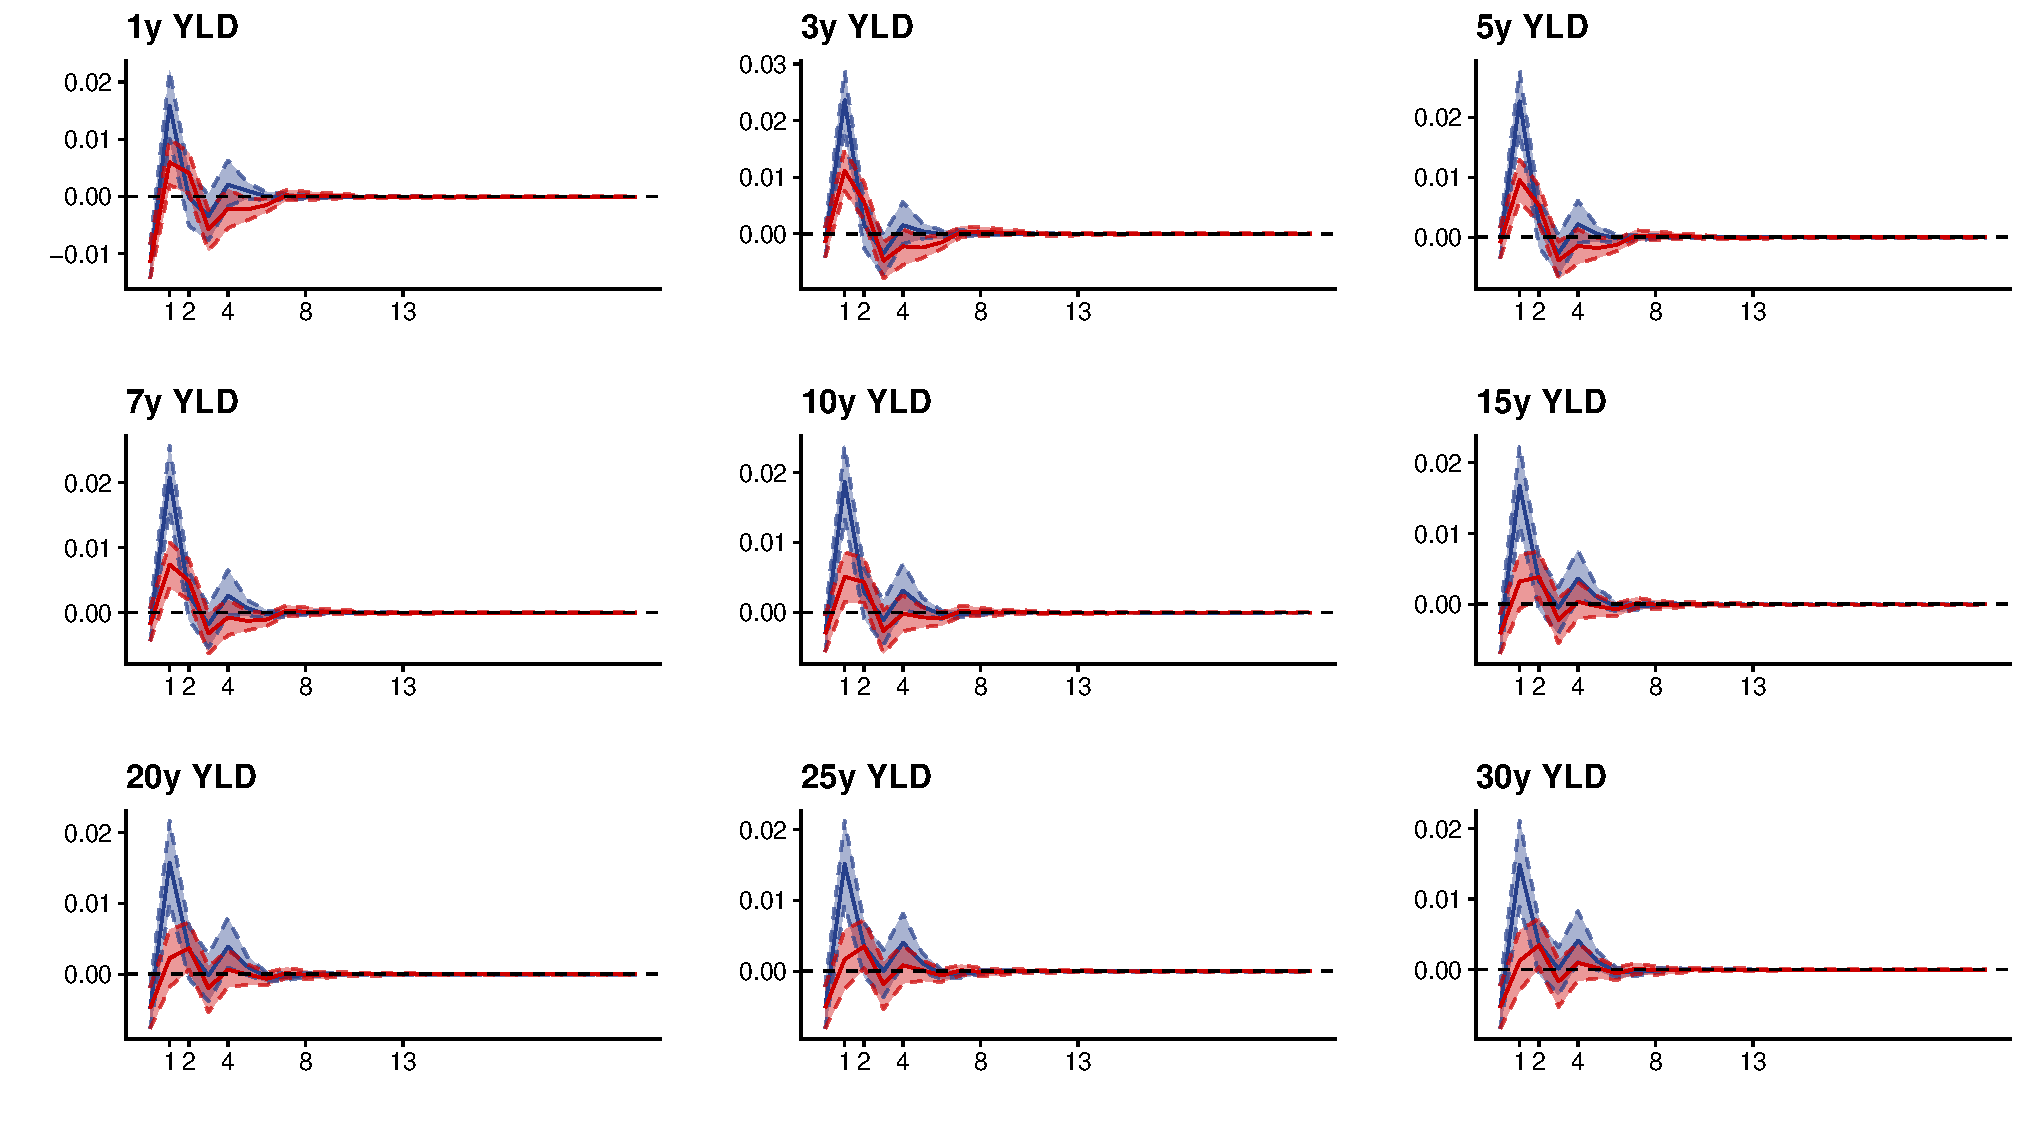
\includegraphics[width=0.85\textwidth]{images_updated/DIFF_EA_Motto/IRF_YLDS_LH_SLCT.pdf}
\end{minipage}
\begin{minipage}{\textwidth}
\centering
b) Difference in responses
\end{minipage}
\begin{minipage}{1\textwidth}
\centering
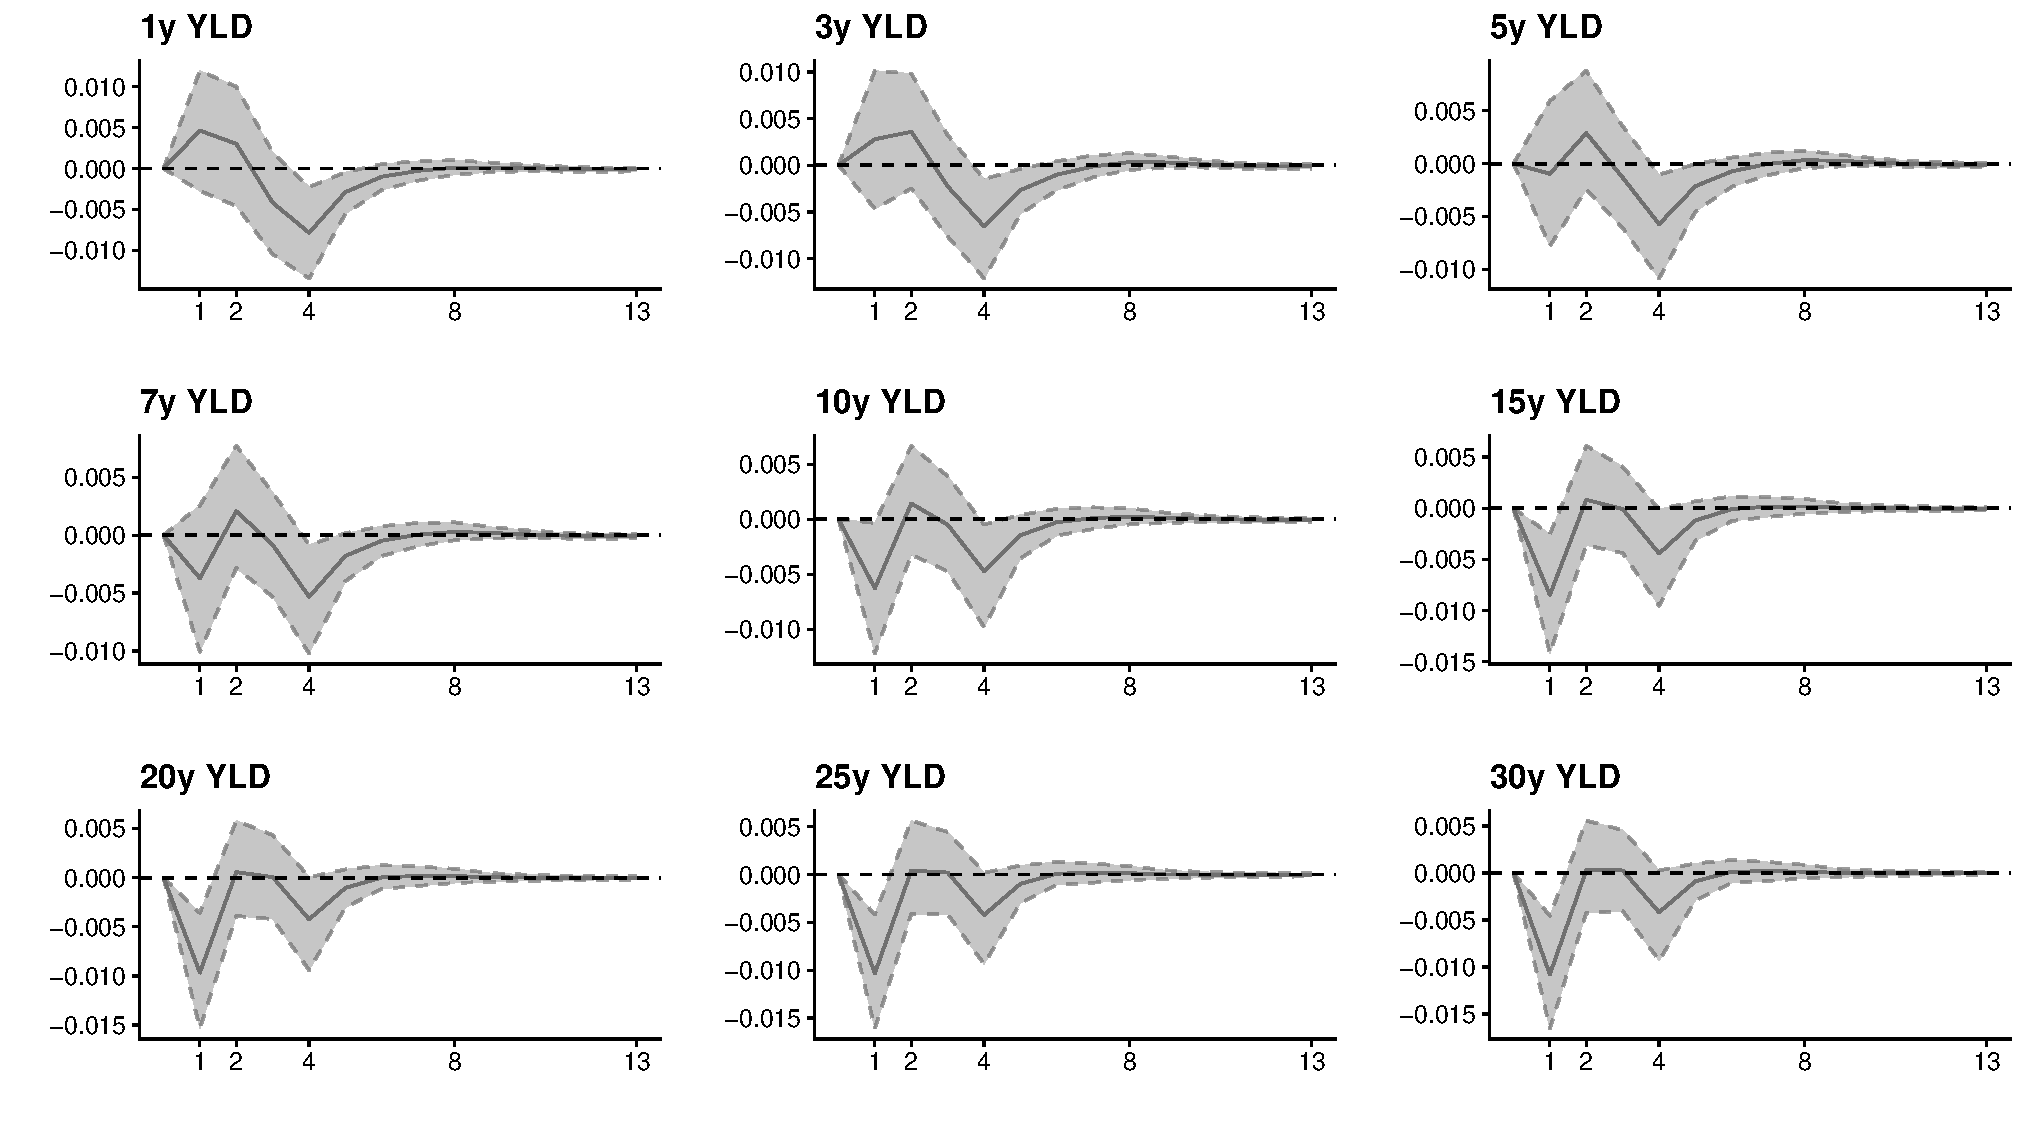
\includegraphics[width=0.85\textwidth]{images_updated/DIFF_EA_Motto/IRF_YLDS_D_SLCT.pdf}
\end{minipage}
\caption*{\footnotesize \textit{Notes:} Panel (a) plots the responses to a contractionary monetary policy shock in the EA conditional on two scenarios: A restrictive US monetary policy stance (95$\%$ percentile of the threshold, colored in red) and an expansionary US monetary policy stance (5$\%$ percentile of the threshold, colored in blue). Panel (b) plots the differences between the two US regimes (restrictive minus expansionary stance). In both panels, the horizontal axis indicates the weeks following the shock. The shaded areas denote the $68\%$ posterior credible set and the solid line denotes the posterior median. Responses are weekly changes in percentage points.}
\end{figure}


Inspecting \autoref{fig:IRFylds}, we find that in both regimes, government bond yields rise on impact after a restrictive monetary policy shock, and in both the reaction is concentrated in the first week and has died out within roughly six weeks. What differs across regimes is the maturity profile. Comparing the blue and red lines in panel (a), the two regimes are statistically indistinguishable at the short end. However, the gap then opens up, and changes sign, as maturity increases. Panel (b) shows this difference to be significantly negative for every maturity from ten years upwards, and insignificant at one, three, and five years. This clean monotone pattern matches the continuum in \autoref{fig:headline} and, hence, the term-premium mechanism that motivates it.  More generally, the two-extreme comparison is illustrative as it contrasts two tail stances. Thus it discards the intermediate observations that carry most of the identifying information, which is why the credible sets in panel (b) are wide beyond the impact week. 



\subsection{Exchange rate, equities, and systemic stress}

Our model also includes the euro--dollar exchange rate, stock market returns, and the CISS. \autoref{fig:IRFOTHER} reports their responses under the two reference stances of the Fed, together with the difference between the two. The Fed's stance matters here too, and in opposite directions for the two asset classes. The euro appreciates by $0.13$ percent one week after a restrictive surprise when the Fed is accommodative, and essentially not at all when the Fed is restrictive, which is what the mechanism of \autoref{fig:headline} implies: a loose Fed leaves more room for an ECB surprise to move the transatlantic differential. The difference between the regimes is not itself statistically significant, however, so we read it as suggestive only. Equities fall by about $0.4$ percent under either stance. The regimes diverge thereafter: one week out the decline has largely reversed under an accommodative Fed, to $0.06$ percent, but persists at $0.15$ percent under a restrictive one, and this difference is significant. That ordering follows the real-rate result rather than the nominal one: an ECB tightening delivered into a tight Fed raises the short real rate by considerably more, and it is the real discount rate that equities price. The systemic stress indicator behaves differently. The CISS rises after a restrictive surprise in both regimes, but by more, and more persistently, when the Fed is \textit{restrictive}. The sign is economically sensible: a domestic tightening that arrives on top of an already tight global financial environment adds to funding stress, whereas the same surprise under an accommodative Fed is cushioned by ample global liquidity. Note also that, since we use only triple-A rated sovereign bonds, safe-haven motives within the euro area play little role in these results.

\begin{figure}[!htpb]
\caption{Impulse responses of a restrictive EA monetary policy shock for other quantities.\label{fig:IRFOTHER}}
\begin{minipage}{\textwidth}
\centering
a) Responses for two scenarios of US monetary policy
\end{minipage}
\begin{minipage}{\textwidth}
\centering
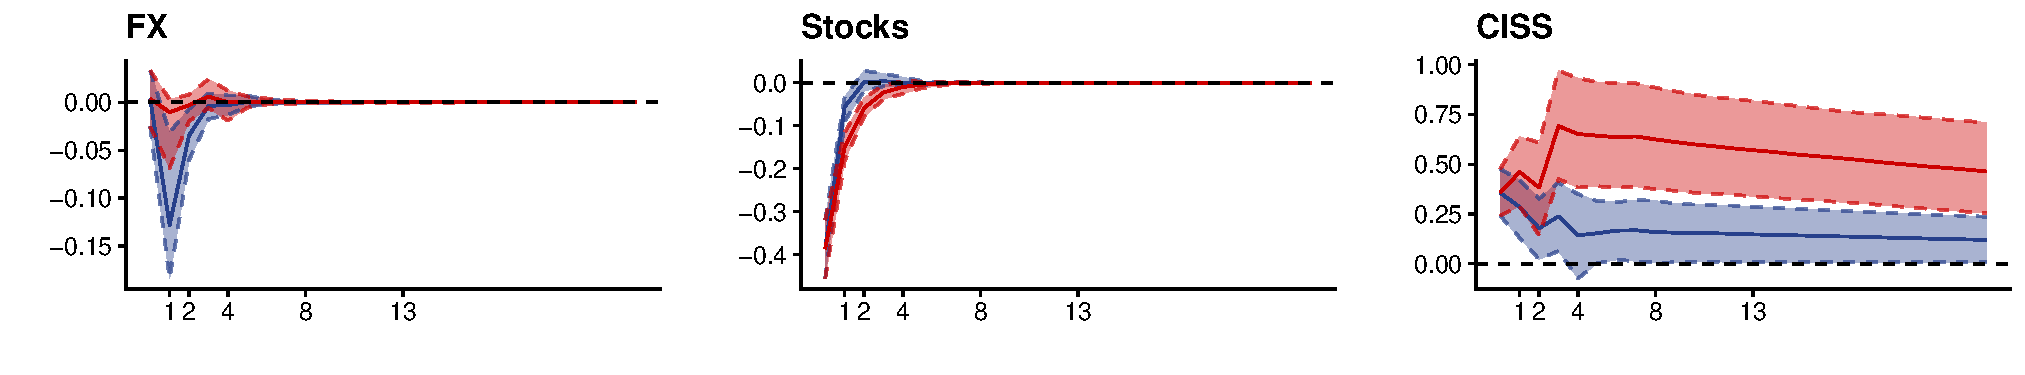
\includegraphics[width= \textwidth]{images_updated/DIFF_EA_Motto/IRFOTHERS_LH.pdf}
\end{minipage}
\begin{minipage}{\textwidth}
\centering
b) Difference in responses
\end{minipage}
\begin{minipage}{1\textwidth}
\centering
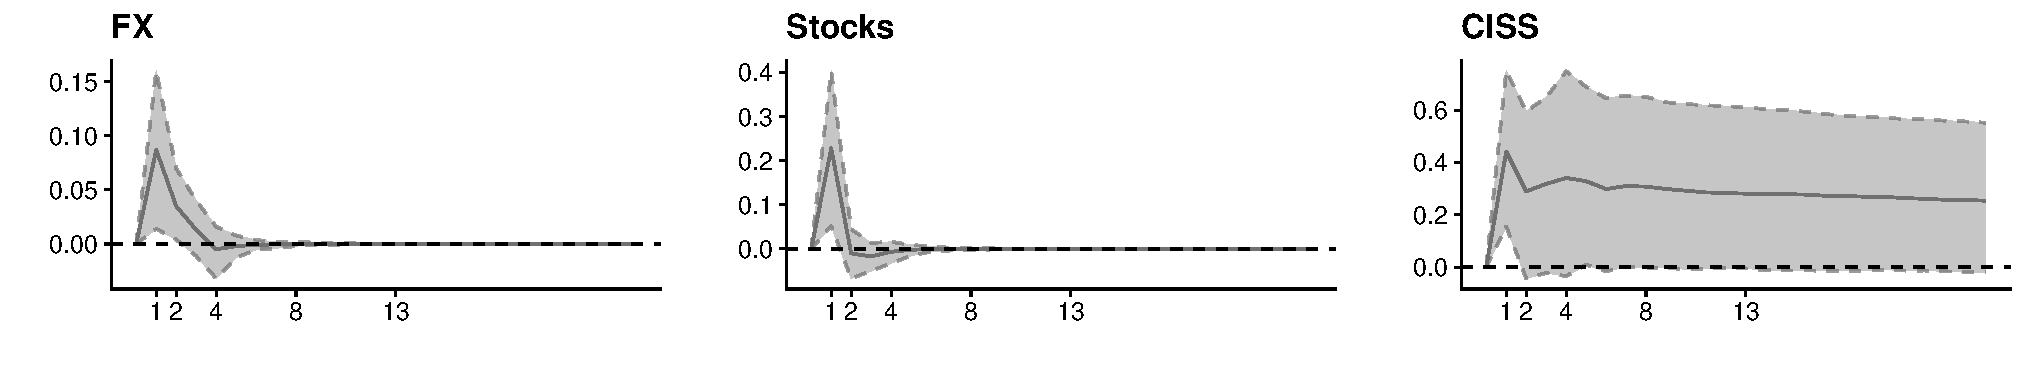
\includegraphics[width= \textwidth]{images_updated/DIFF_EA_Motto/IRFOTHERS_D.pdf}
\end{minipage}
\caption*{\footnotesize \textit{Notes:} Panel (a) plots the responses to a contractionary monetary policy shock in the EA conditional on two scenarios: A restrictive US monetary policy stance (95$\%$ percentile of the threshold, colored in red) and an expansionary US monetary policy stance (5$\%$ percentile of the threshold, colored in blue). Panel (b) plots the differences between the two US regimes (restrictive minus expansionary stance). In both panels, the horizontal axis indicates the weeks following the shock. The shaded areas denote the $68\%$ posterior credible set and the solid line denotes the posterior median. FX denotes the Euro per one US-dollar (i.e., a decrease denotes an appreciation of the Euro), Stocks the Euro Stoxx 50 index, and CISS the Composite Index of Systemic Stress.}
\end{figure}


% {\color{red}
% \subsection{Controlling for global factors}\label{sec:global}
% A natural concern with our identification strategy is that the Fed's stance may partly reflect common global conditions rather than US monetary policy per se. During a synchronized global inflation cycle, for instance, the Fed may be tight at the same time as commodity prices, the dollar, and global risk aversion move, and it could be these global forces, rather than US policy, that alter the transmission of ECB surprises. We address this concern in two complementary ways.

% First, we augment the vector $\bm y_t$ with three global variables that are available at daily frequency and span the main dimensions of the global cycle: the Brent oil price (in percentage changes), the broad nominal US dollar index (in percentage changes), and the VIX as a proxy for global risk aversion. These variables enter both regimes and are allowed to react to, and feed back into, all EA quantities. \autoref{fig:IRFglobal} shows the yield curve responses from this extended model. They are remarkably close to the baseline: yield reactions to a restrictive ECB surprise remain significantly stronger under an accommodative Fed, with the one-week-ahead difference at short maturities significant at the $68\%$ level, and the maturity profile of the differences is unchanged. The global variables themselves react little to the ECB surprise, consistent with the euro area being small relative to global financial markets.

% Second, we purge the stance measure itself of the global cycle. We regress $z_t^{\ast}$ on year-on-year oil price growth, year-on-year growth of the broad dollar index, and the level of the VIX, and use the residual --- the component of the Fed's stance that is orthogonal to these global factors --- as the transition variable. The resulting regime allocation is nearly identical to the baseline (the correlation of the posterior mean of $S_t$ across the two specifications is $0.95$), confirming that our stance measure is not simply a repackaged global cycle. The impulse responses retain the same pattern, although the differences between regimes lose some statistical precision, which is expected given that the purging step removes variation that is informative about the stance itself. Taken together, these exercises indicate that the state dependence we document is attributable to the US policy stance and not to omitted global variables, although we acknowledge that no reduced-form exercise can fully isolate US monetary policy from the global conditions to which it responds.

% \begin{figure}[!htpb]
% \caption{\rev{Impulse responses of government bond yields in the model with global variables.} \label{fig:IRFglobal}}
% \begin{minipage}{\textwidth}
% \centering
% a) Responses for two scenarios of US monetary policy
% \end{minipage}
% \begin{minipage}{\textwidth}
% \centering
% 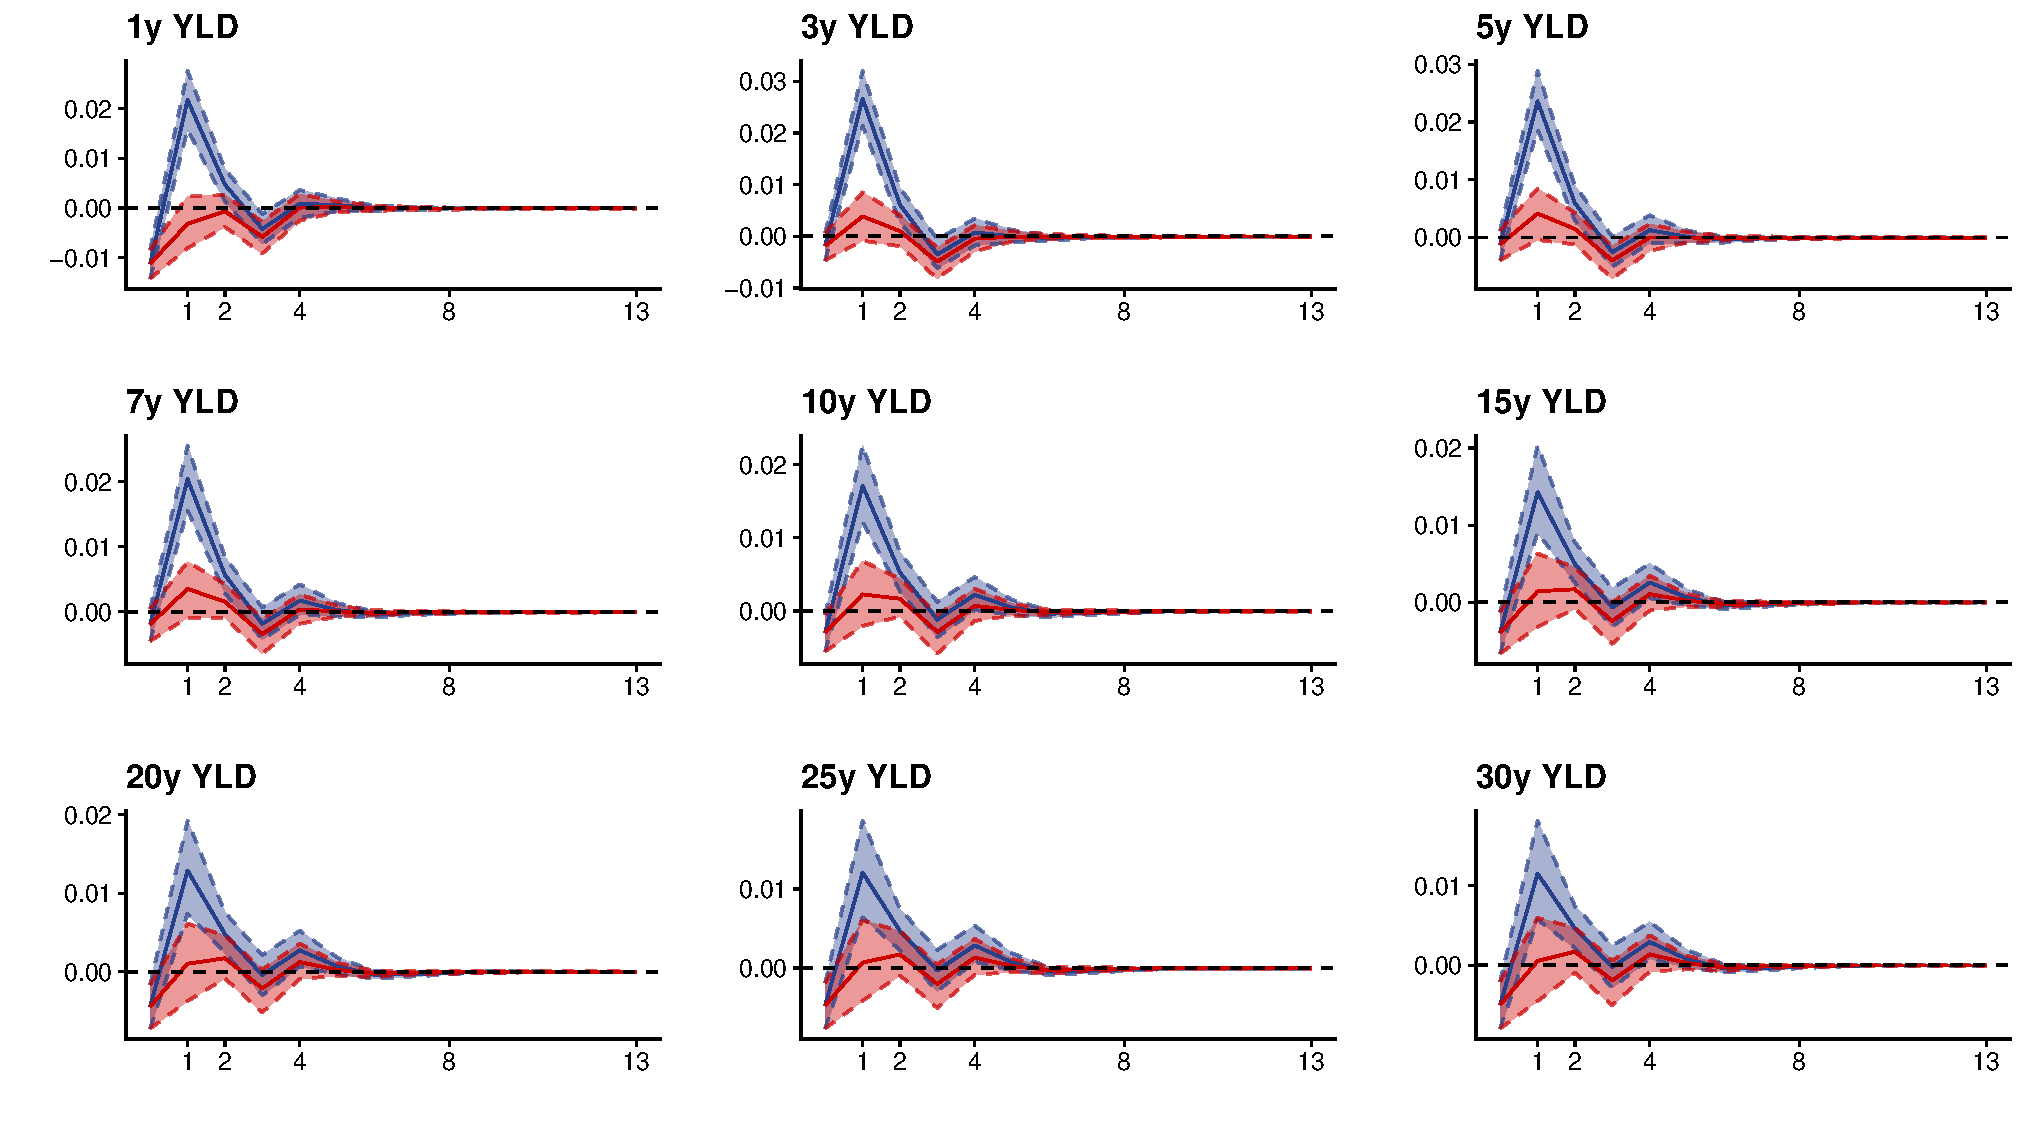
\includegraphics[width=0.7\textwidth]{images/rev/IRF_YLDS_GLOB19_LH_SLCT.pdf}
% \end{minipage}
% \begin{minipage}{\textwidth}
% \centering
% b) Difference in responses
% \end{minipage}
% \begin{minipage}{1\textwidth}
% \centering
% 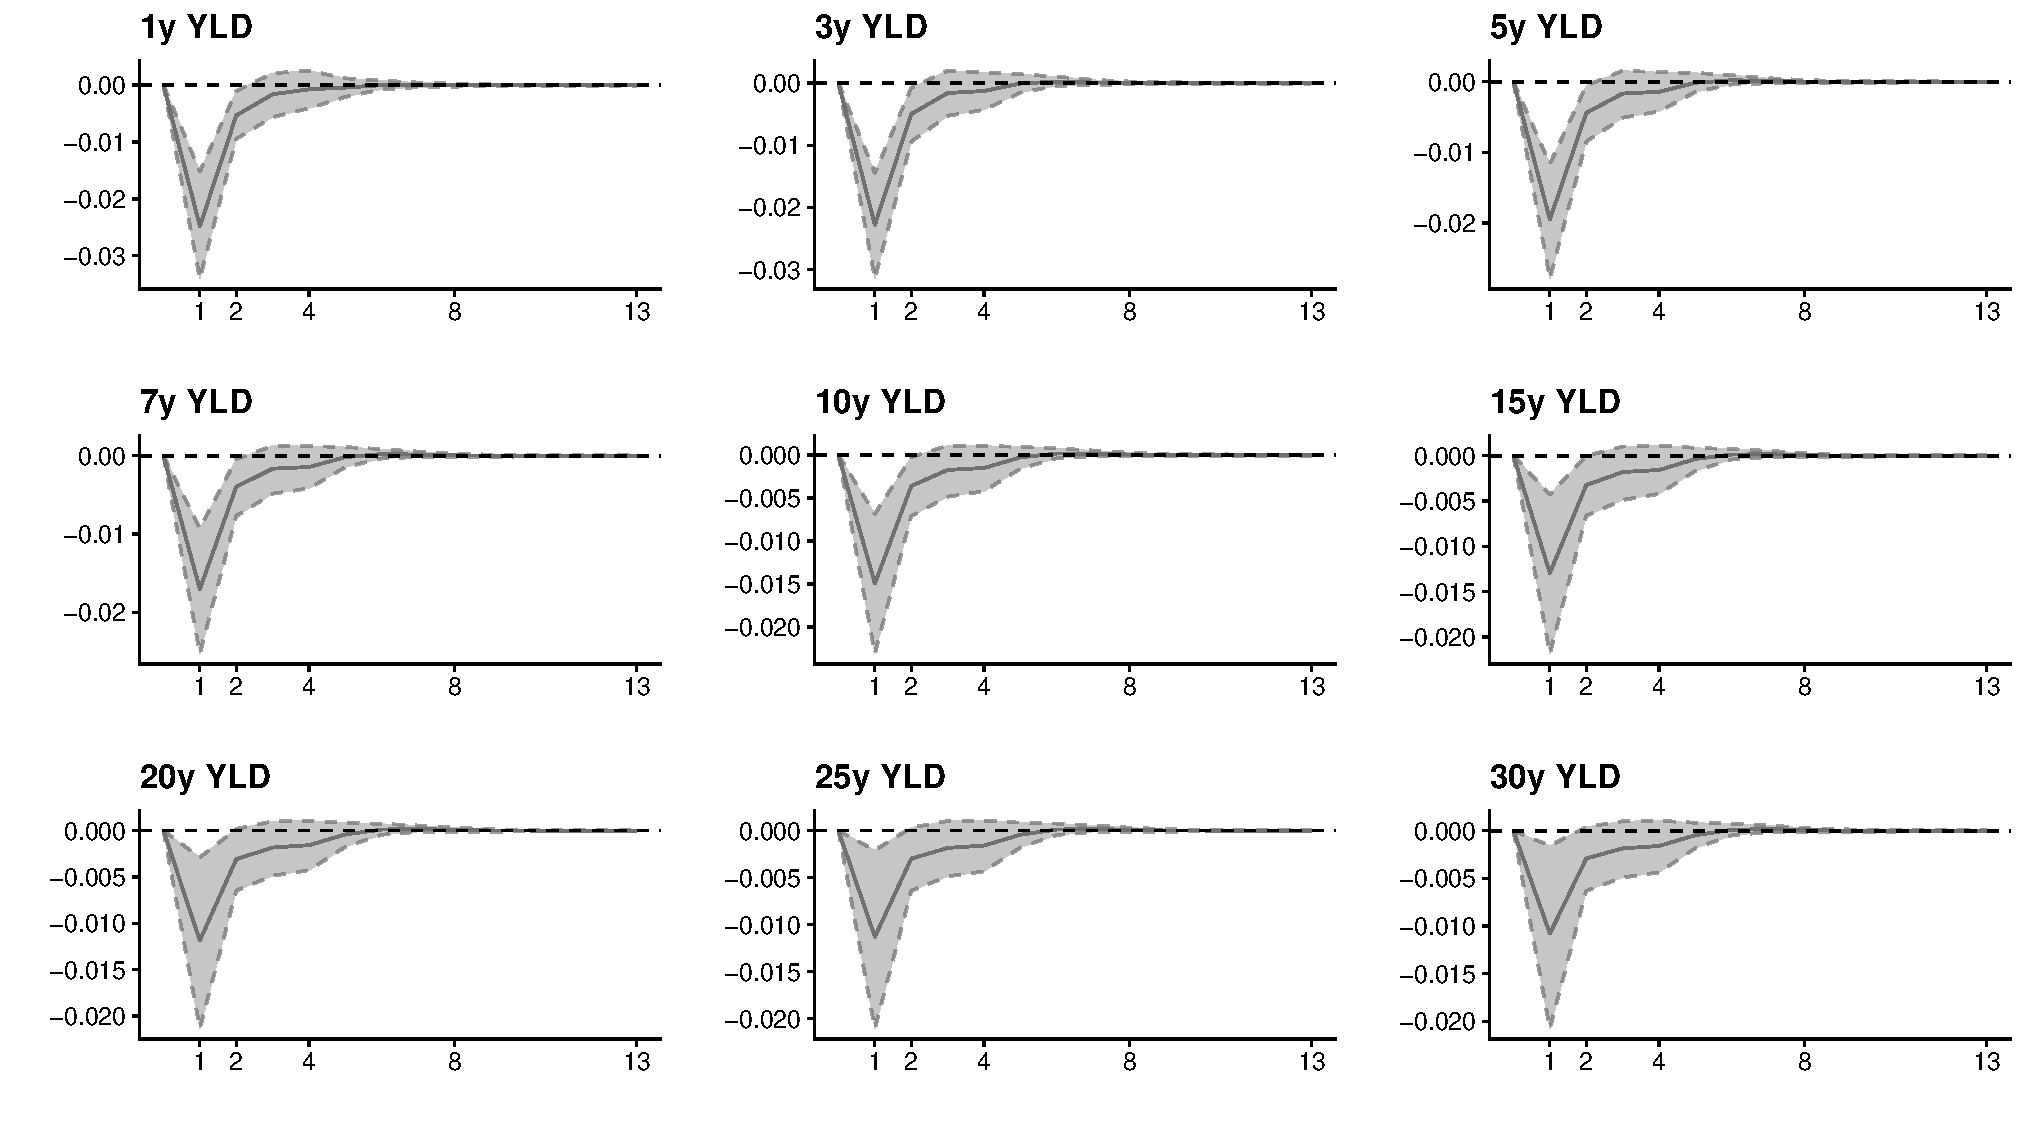
\includegraphics[width=0.7\textwidth]{images/rev/IRF_YLDS_GLOB19_D_SLCT.pdf}
% \end{minipage}
% \caption*{\footnotesize \textit{Notes:} \rev{Responses to a contractionary EA monetary policy shock in the specification that augments $\bm y_t$ with the Brent oil price, the broad US dollar index, and the VIX, estimated over the full 2005--2026 sample. Panel (a) conditions on a restrictive (95\% percentile, red) and an expansionary (5\% percentile, blue) US stance; panel (b) shows the difference (restrictive minus expansionary). Shaded areas denote the 68\% posterior credible set.}}
% \end{figure}




\subsection{Robustness}\label{sec:results_rob}
The rotation documented above rests on two constructed inputs and two  parameters. The stance measure decides \textit{when} the Fed is restrictive, thus impacting the state allocation, while the monetary policy surprise measure decides \textit{what} an ECB policy shock is, impacting the dynamic responses. Finally, the transition parameters $\mu$ and $\rho$ fix the location and sharpness of the boundary between regimes. For robustness checks, we vary each in turn, holding the others at baseline. Appendix~\ref{app:rob} collects the results with an overview of the specifications in \autoref{tab:robspecs}.

%Replacing the stance with the shadow short rate of \cite{krippner2016ems} relative to $r^{\ast}$ leaves the regime dating essentially untouched: the two posterior transition paths correlate at $0.95$, and both assign $41.0\%$ of weeks to the restrictive regime. Replacing the identification with the median-rotation shocks of \cite{jarocinski2020deconstructing} changes the impulse itself and is the more demanding test. Moving the neutral cut by a quarter and by half a percentage point of the stance reclassifies up to $148$ of $1{,}090$ weeks and shifts the restrictive share from $34.8\%$ to $54.6\%$; the sustained restrictive phase from mid-2022 to the end of the sample stays restrictive under every cut. Centering the steepness prior at seven rather than four leaves the responses virtually unchanged (correlation of posterior medians $0.998$, maximum deviation $0.17$ basis points).

The results are robust to alternative measures of the policy stance, identification schemes, regime thresholds, and prior specifications. Although these choices affect the classification of some weeks and, in the case of alternative shocks, the estimated impulse itself, the main pattern of a sustained restrictive US monetary policy stance since mid-2022 and the resulting impulse responses remains unchanged.

Across all eight specifications, the rotation is preserved. Short-maturity responses are significantly positive across the entire stance distribution after a restrictive EA MP shock, whereas long-maturity responses become insignificant under sufficiently restrictive US monetary policy. The loose-minus-tight differential is negative at short maturities, close to zero in the belly of the curve, and positive and increasing from ten years onward. Thus, the sign and maturity profile of the state dependence are robust to alternative measurements, calibrations, and identification schemes.


%Across all eight specifications the rotation is present without exception. The response at short maturities is significantly positive at every point of the stance distribution, while at thirty years it ceases to be so somewhere between the fifty-fifth and the seventieth percentile in every one of the eight. The gap between the regimes is negative at one year, indistinguishable from zero in the belly of the curve, and positive and increasing in maturity from ten years out, in every specification. The sign and the maturity profile of the state dependence are therefore not artifacts of measurement or calibration: the posterior probability of a positive loose-minus-tight gap at thirty years is at least $0.88$ in seven of the eight specifications and $0.81$ in the remaining one, which replaces our composite surprise with the alternative identification.

%%% [superseded by the following paragraph -- commented out 2026-07-27] Its magnitude is more sensitive, and we are correspondingly careful with it. The thirty-year gap ranges from $0.48$ basis points under the alternative identification to $1.22$ under the widest regime definition. Most of that range is attributable to the identification of the surprise rather than to the calibration: across the four alternative cuts the gap varies only between $0.79$ and $1.22$ basis points, and lowering the cut widens it monotonically, since a lower cut confines the accommodative state to more deeply accommodative weeks. For the same reason we attach no interpretation to the shape of the accommodative-Fed profile in \autoref{fig:headline}, which tilts in either direction under modest changes in the cut: what is robust is the \textit{contrast} between the two states, not the shape of the response within either. We therefore read the evidence as establishing that euro area long-rate pass-through is weaker when the Fed is restrictive, and we report the size of that difference as a range rather than a point estimate.

The magnitude of the effect is more sensitive. At the thirty-year maturity, the loose-minus-tight gap ranges from $0.48$ to $1.22$ basis points, with most variation attributable to the identification of the policy surprise rather than to alternative regime definitions. We therefore refrain from interpreting the precise shape of responses within the accommodative state. The robust finding is instead the contrast across states: euro area long-rate pass-through is weaker when the Fed is restrictive. We consequently report the estimated difference as a range rather than a point estimate.




\section{Concluding remarks}\label{sec:conclusio}
\rev{In a globalised world, monetary policy depends not only on prevailing macroeconomic fundamentals but also on how central banks interact, because key transmission channels have an explicit international dimension and effective policy hinges on international spillovers in financial and real markets as much as on domestic first-round effects. In this paper, we develop an empirical weekly time series model that captures, in a nonlinear fashion, the interactions between domestic macro-financial dynamics in the euro area (EA) and the US monetary policy stance. We identify shocks using readily available high-frequency instruments designed to capture unexpected movements in monetary policy, and we measure the US policy stance from an estimate of the neutral interest rate.}

\rev{In sum, our results reveal a systematic interaction between US and EA monetary policy. Rather than relying on a comparison of two extreme stances, we characterise the transmission of an ECB surprise across the entire range of the Fed's stance. For nominal bond yields this mapping is clean and monotone: a contractionary EA surprise raises euro area yields significantly when the Fed is accommodative, and this reaction weakens steadily as the Fed turns restrictive, vanishing or reversing at long maturities under a strongly hawkish Fed.} These effects reverse after about two weeks. At this horizon, bond yields tend to fall in response to capital inflows into the EA economy, which pushes up bond prices. In contrast, when the EA shock occurs under a restrictive Fed stance, we observe somewhat weaker reactions with heterogeneity across maturities. Looking at the reactions of the inflation swap curve, we observe muted differences when controlling for the US stance. In general, the results point to negative reactions at impact, with different dynamics thereafter depending on the prevailing US monetary policy stance. However, even though they are marginally significant, there is some evidence of nonlinearities.
\rev{Finally, our model lets us examine real interest rate reactions by taking the difference between the nominal-yield and inflation-swap IRFs; these suggest that real rates rise in all scenarios, though more so when EA shocks occur during a restrictive Fed stance.}

\rev{The revision of this paper has substantially broadened the evidence behind these conclusions. The state dependence with respect to the Fed's stance survives the inclusion of global variables (oil, the broad dollar, and global risk aversion) and the use of a stance measure purged of the global cycle; it is empirically distinct from state dependence on the euro area business cycle, as the regime allocations implied by the two conditioning variables are essentially uncorrelated; it is present for both tightening and easing surprises; and it is estimated on a sample running through the end of 2025 that covers the post-pandemic global tightening, during which the model identifies a pronounced restrictive Fed regime for 2022--2024 that sharpens the identification of the state dependence. Moreover, since the model is specified in first differences, the fast mean reversion of the reported responses translates into persistent level effects on yields, with the sign of the long-run level effect itself depending on the Fed's stance.}

\rev{The model interacts foreign monetary policy with domestic quantities in a simple and transparent way. A natural next step is to relax the logistic form of the interaction and let the data determine how the transmission depends on the Fed's stance --- for instance through a time-varying parameter VAR whose coefficients are nonparametric functions of the stance, modelled with regression trees \citep{hauzenberger2025bayesian}. Such an approach would accommodate richer, potentially non-monotone patterns of state dependence than the two-regime mixture imposed here.} In addition, we have only included EA-based quantities and capture international spillovers mainly by including the US monetary policy stance. Estimating larger bi-country models would in principle be feasible, which we leave for further research.




\section*{Conflicts of Interest}
The authors have no relevant financial or non-financial interests to
disclose.

% Bibliography
\newpage
\small{\scfont\setstretch{0.85}
\addcontentsline{toc}{section}{References}
\bibliographystyle{custom.bst}
\bibliography{lit_updated}}

\clearpage % ensure all floats are processed
%\processdelayedfloats

% Appendices
\begin{appendices}

\setcounter{equation}{0}
\renewcommand\theequation{A.\arabic{equation}}
\setcounter{table}{0}
\renewcommand{\thetable}{A\arabic{table}}

\section{Data}\label{app:0}
%\subsection{Appendix 0}\label{app:0}



\begin{table}[!htbp]
{\tiny
\caption{Data description \label{tab:data}} 
\begin{tabular}{llllll}
\toprule
& \textbf{Label}  & \textbf{Mnemonic} & \textbf{Description}  & Frequency & \textbf{Transformation}   \\ 
\midrule
\multicolumn{6}{c}{(a) Euro Area}\\[0.5em]
& Yields & $\texttt{YLD}^{\tau Y}$ & EA government bond yields (AAA-rated)  with maturity $\tau$ years ahead & daily, aggregated to weekly & first differences\\
& ILS & $\texttt{INFSWP}^{\tau Y}$ & Inflation-linked swaps $\tau$- year ahead & daily, aggregated to weekly & first differences\\
& EuroStoxx50 & $\texttt{Stocks}$ & Euro area stock market index   & daily, aggregated to weekly & percentage changes \\
& CISS & $\texttt{CISS}$ & Euro area composite indicator of systemic stress \citep{kremer2012CISS} & daily, aggregated to weekly & first differences \\
& EUR-USD Exchange Rate & $\texttt{FX}$ & Exchange rate in EUR per USD & daily, aggregated to weekly &  percentage changes\\ \\
\midrule
 \multicolumn{6}{c}{(b) United States}\\[0.5em]
 & Neutral rate   & $r^{\ast}$ &  estimate of the natural rate of interest \citep{laubach2003measuring} &  quarterly, interpolated to weekly  & level  (One-sided) \\
& Policy Rate & \texttt{DFF} &  Federal Funds Effective Rate  &daily, aggregated to weekly &level \\
& Effective Monetary Stimulus & \texttt{EMS} &  Effective Monetary Stimulus \citep{krippner2016ems} &daily, aggregated to weekly &level\\
& Shadow Short Rate & \texttt{SSR} & Shadow Short Rate \citep{krippner2016ems} &daily, aggregated to weekly &level\\
\midrule
 \multicolumn{6}{c}{\color{red}(c) Global variables (used in the global-controls robustness specification, \autoref{app:rob})}\\[0.5em]
& \color{red} Oil price & \color{red}\texttt{OIL} & \color{red} Brent crude oil spot price (FRED: DCOILBRENTEU) & \color{red} daily, aggregated to weekly & \color{red} percentage changes\\
& \color{red} US dollar index & \color{red}\texttt{USD} & \color{red} Broad nominal US dollar index (FRED: DTWEXBGS, spliced with DTWEXM before 2006) & \color{red} daily, aggregated to weekly & \color{red} percentage changes\\
& \color{red} VIX & \color{red}\texttt{VIX} & \color{red} CBOE volatility index (FRED: VIXCLS) & \color{red} daily, aggregated to weekly & \color{red} percentage changes\\
& \color{red} Weekly activity & \color{red}\texttt{WAI} & \color{red} Bundesbank weekly activity index for Germany (used in \autoref{app:rob}) & \color{red} weekly & \color{red} level\\
\bottomrule
\end{tabular}}
\begin{minipage}{\textwidth}
\vspace{0.1cm}
\scriptsize \textbf{Notes:} The inflation-linked swaps are gathered from Macrobond, while the remaining EA variables are obtained from the ECB's Statistical Data Warehouse (\href{https://sdw.ecb.europa.eu/}{https://sdw.ecb.europa.eu/})\rev{, now the ECB Data Portal (\href{https://data.ecb.europa.eu/}{data.ecb.europa.eu})}.  For computing the US monetary policy stance, we obtained the \texttt{DFF} from the FRED database of the Federal Reserve Bank of St. Louis (\href{https://fred.stlouisfed.org}{fred.stlouisfed.org}) and the real rate estimate of \cite{laubach2003measuring} from the database of the Federal Reserve Bank of New York (\href{https://www.newyorkfed.org/research/policy/rstar}{www.newyorkfed.org/research/policy/rstar}). The latter is available on a quarterly basis and was interpolated to match weekly frequency. All remaining variables were obtained on a daily basis and then aggregated to weekly frequency by taking the average. Both alternative US monetary policy measures are available on a daily basis and were downloaded from \href{https://www.ljkmfa.com/}{https://www.ljkmfa.com/}. \rev{All series are drawn from the data vintage of July 2026. Specifically, the natural rate is the COVID-adjusted estimate published by the Federal Reserve Bank of New York (through 2026:Q1); the policy surprise factors are the October 2025 vintage (see the footnote in \autoref{sec:measuring}); the aggregate CISS is spliced with its updated composite after May 2025; and the EONIA series is continued with the euro short-term rate (EuroSTR) plus 8.5 basis points following its discontinuation in January 2022. The euro area inflation-linked swap panel spans the entire sample period, so that the full system---bond yields, inflation swaps, and the macro-financial block---is estimated jointly on the single sample running from $2005$:W$1$ to the end of $2025$. The two alternative US stance metrics (\texttt{SSR} and \texttt{EMS}) are taken from the June 2026 vintage of the same source and likewise cover the full sample.}
\end{minipage}
\end{table}



% \begin{table}[h!]
% \centering
% \footnotesize
% \caption{Variable Definitions.}\label{tab:vardef}
% \begin{tabular}{llp{7cm}p{4cm}l}
%   \toprule
%   Label & \textbf{Mnemonic} & Details & Source & Transformation\\
%   \midrule
%   \textbf{Euro Area} & & & & &\\[-0.5ex]
%   \midrule
%   $YLD$ & $\texttt{YLD}^{\tau Y}$ & EA government bond yields (AAA-rated)  with $\tau \in \{1:10,12,15,20,25,30\}$ year ahead & SDW ECB  &  level\\
  
%     $\bm{\pi}^e_t$ & $\texttt{INFSWP}^{\tau Y}$ & inflation linked swaps with $\tau \in \{1:10,12,15,20,25,30\}$ year ahead & Macrobond &\\

%      EuroStoxx50 & $\texttt{Stocks}$ & inflation linked swaps with $\tau \in \{1:10,12,15,20,25,30\}$ year ahead & SDW ECB& \\

%   Composite Indicator of Systemic Stress & $\texttt{CISS}$ & inflation linked swaps with $\tau \in \{1:10,12,15,20,25,30\}$ year ahead & SDW ECB & \\

%   USD-EUR Exchange Rate & $\texttt{FX}$ & inflation linked swaps with $\tau \in \{1:10,12,15,20,25,30\}$ year ahead & SDW ECB &\\
  

%       \textbf{sr}$_t$ & \texttt{SR} & Shadow rate for euro area by \citet{wu2016measuring} & website of Jing Cynthia Wu \\
%   $\bm{\pi}_t$ & $100 \times \ln \left(\frac{\texttt{HICP}_t}{\texttt{HICP}_{t-12}}\right)$ & year-on-year growth rate of harmonized index of consumer prices & constructed \\

%    \midrule
%   \textbf{United States} & & &&\\[-0.5ex]
%   \midrule 
% Fed policy stance$_t$ & \texttt{z_{US}} & Shadow rate for euro area by \citet{wu2016measuring} & website of Jing Cynthia Wu& \\

  
%   \bottomrule
% \end{tabular}
% \end{table}
\newpage
\section{Further empirical results}\label{app:A}
%\subsection{Appendix 1}\label{app:A1}

The following four figures complement the dynamic analysis of \autoref{sec:results}. \autoref{fig:continuumheat} shows the full results of the one-week-ahead ($h=1$) response of the government bond yield at each maturity to a one-standard-deviation restrictive ECB surprise, evaluated at each percentile of the US monetary policy stance. \autoref{fig:IRFswps} and \autoref{fig:IRFreal} report the dynamic responses of inflation swaps and real yields under the two reference stances of the Fed, whose one-week-ahead behavior across the full stance continuum is summarized in \autoref{fig:headline} in the main text.

\begin{figure}[!htpb]
\centering
\caption{Heatmap of one-week-ahead response of the full government bond yield curve to a restrictive ECB surprise, across all percentiles of the Fed's monetary policy stance.\label{fig:continuumheat}}
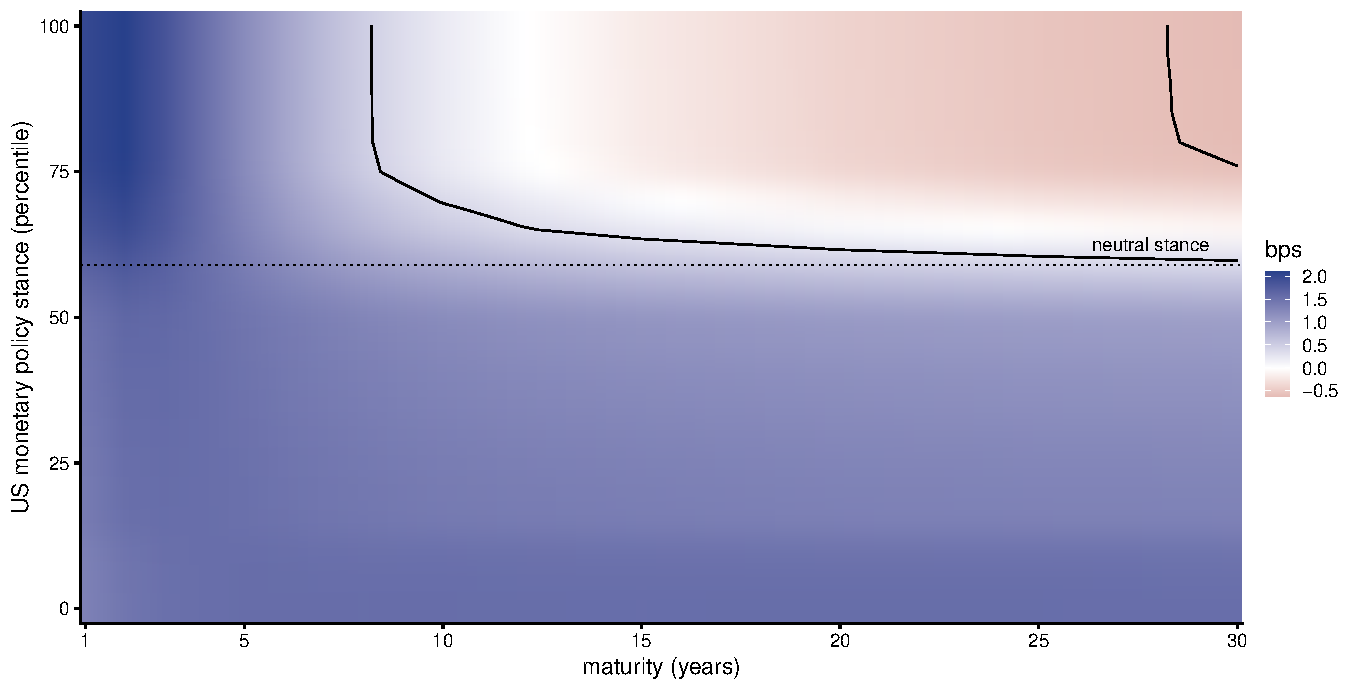
\includegraphics[width=\textwidth]{images_updated/rev/IRF_termstructure_continuum.pdf}
\caption*{\footnotesize \textit{Notes:} Posterior median of the one-week-ahead ($h=1$) response (in basis points, color scale) of the government bond yield at each maturity (horizontal axis, 1-30 years) to a one-standard-deviation restrictive ECB surprise, evaluated at each percentile of the US monetary policy stance $z^\ast_t$ (vertical axis; 0 = most accommodative, 100 = most restrictive week in the sample). The solid contour delimits the region in which the $68\%$ posterior credible set no longer excludes zero (upper right); the dotted horizontal line marks the percentile at which the stance crosses zero, i.e., the calibrated regime threshold. Responses at maturities between the 15 estimated grid points are linearly interpolated. Estimated on the nominal bond term structure over the full sample, 2005:W1-2025:W52.}
\end{figure}

The swap responses are an order of magnitude smaller than the yield responses and, beyond the impact week, the differences across Fed regimes are imprecisely estimated; the real-yield dynamics closely track the nominal ones. \autoref{fig:IRFcum} accumulates the weekly yield responses and displays the implied \textit{level} effects: since the model is specified in first differences of the term structure factors, a differenced response that returns to zero does not mean the effect on yields disappears, but that yields settle at a new level. Under an accommodative Fed, yields of three years and above settle about two basis points higher and the effect does not unwind over the 26-week horizon; under a restrictive Fed no lasting level effect remains, and the cumulated response of the one-year yield even drifts slightly negative, which is the level counterpart of the short-end reversal discussed in the main text.

\begin{figure}[!htpb]
\caption{Impulse responses of a restrictive EA monetary policy shock for selected \textit{inflation swaps}.\label{fig:IRFswps}}
\begin{minipage}{\textwidth}
\centering
a) Responses for two scenarios of US monetary policy
\end{minipage}
\begin{minipage}{\textwidth}
\centering
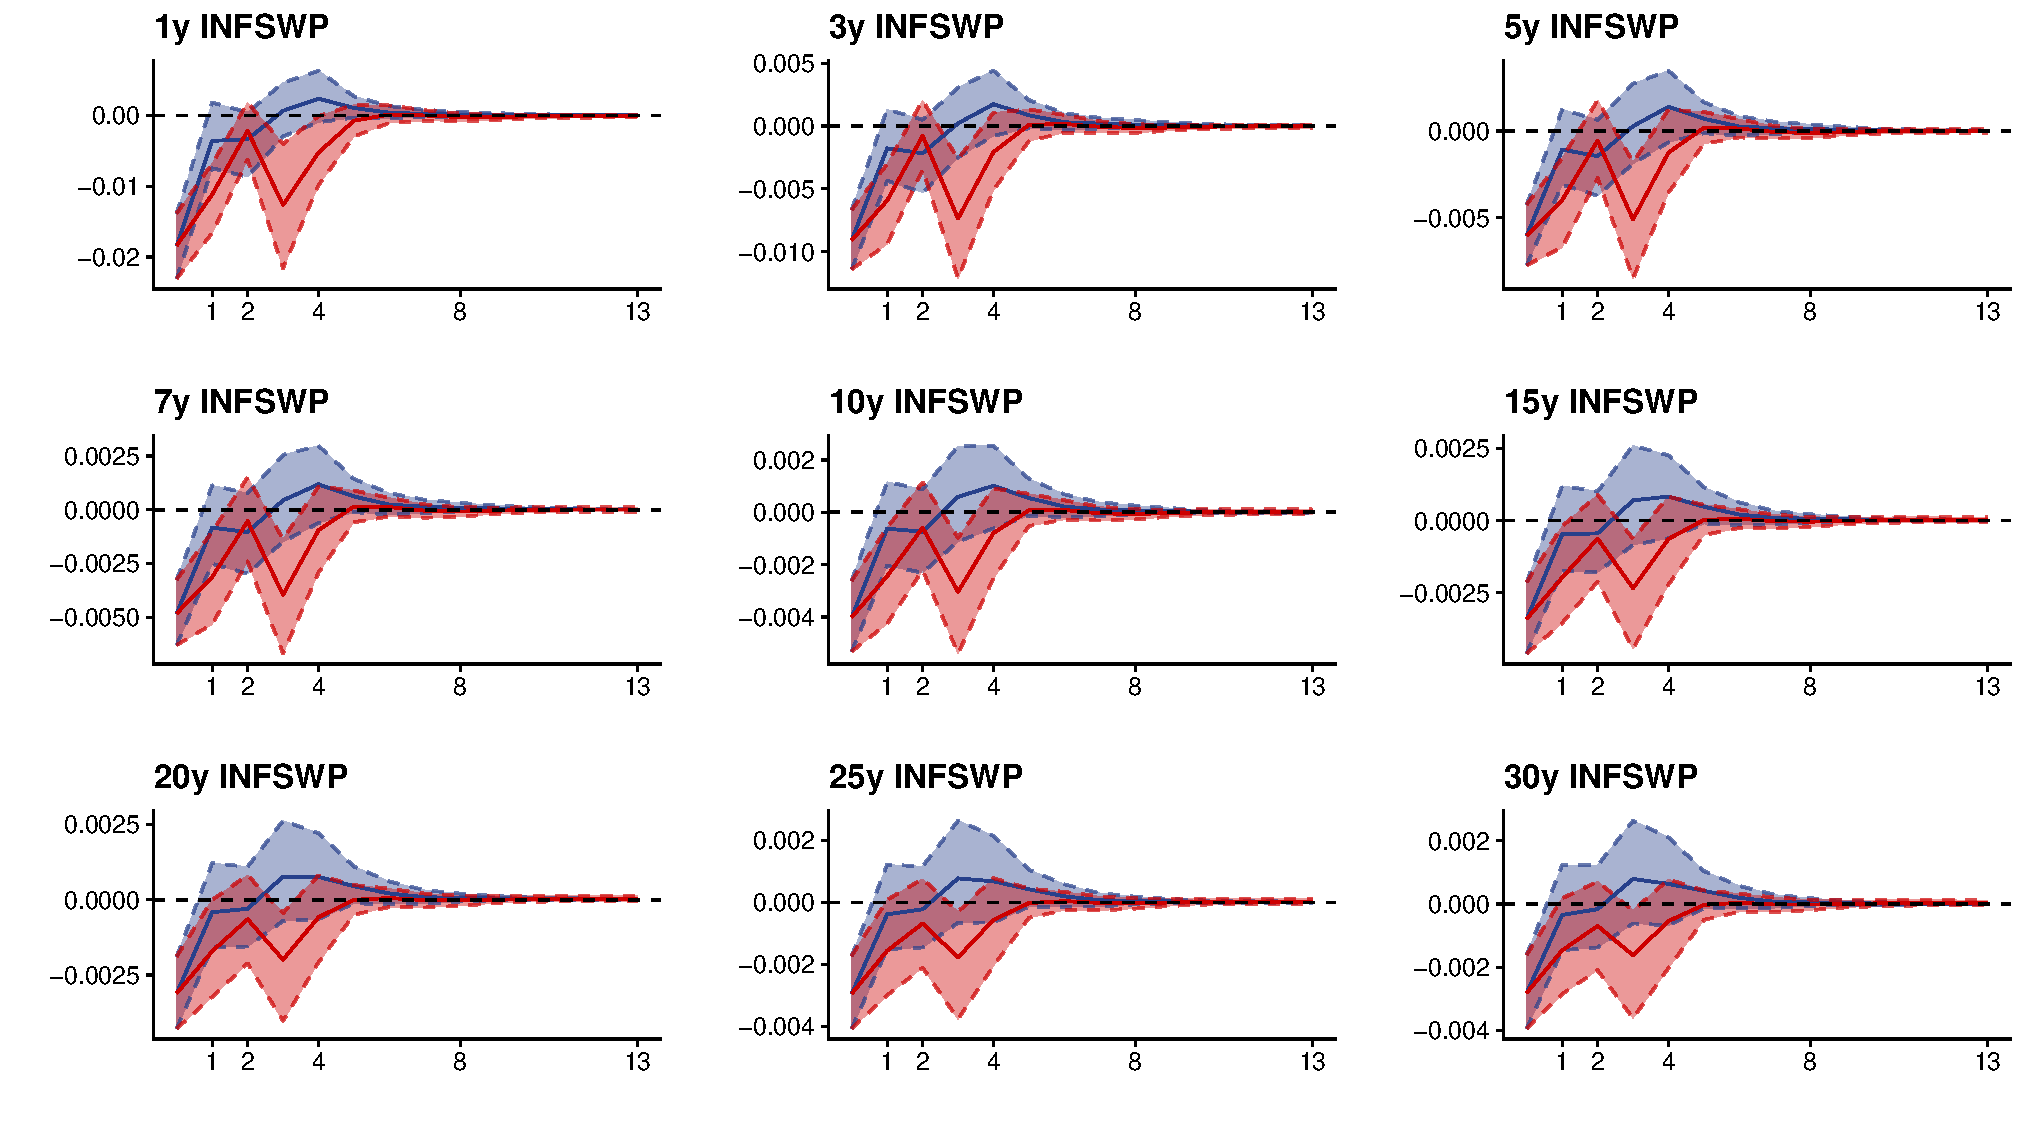
\includegraphics[width= 0.7\textwidth]{images_updated/DIFF_EA_Motto/IRF_INFSWP_LH_SLCT.pdf}
\end{minipage}
\begin{minipage}{\textwidth}
\centering
b) Difference in responses
\end{minipage}
\begin{minipage}{1\textwidth}
\centering
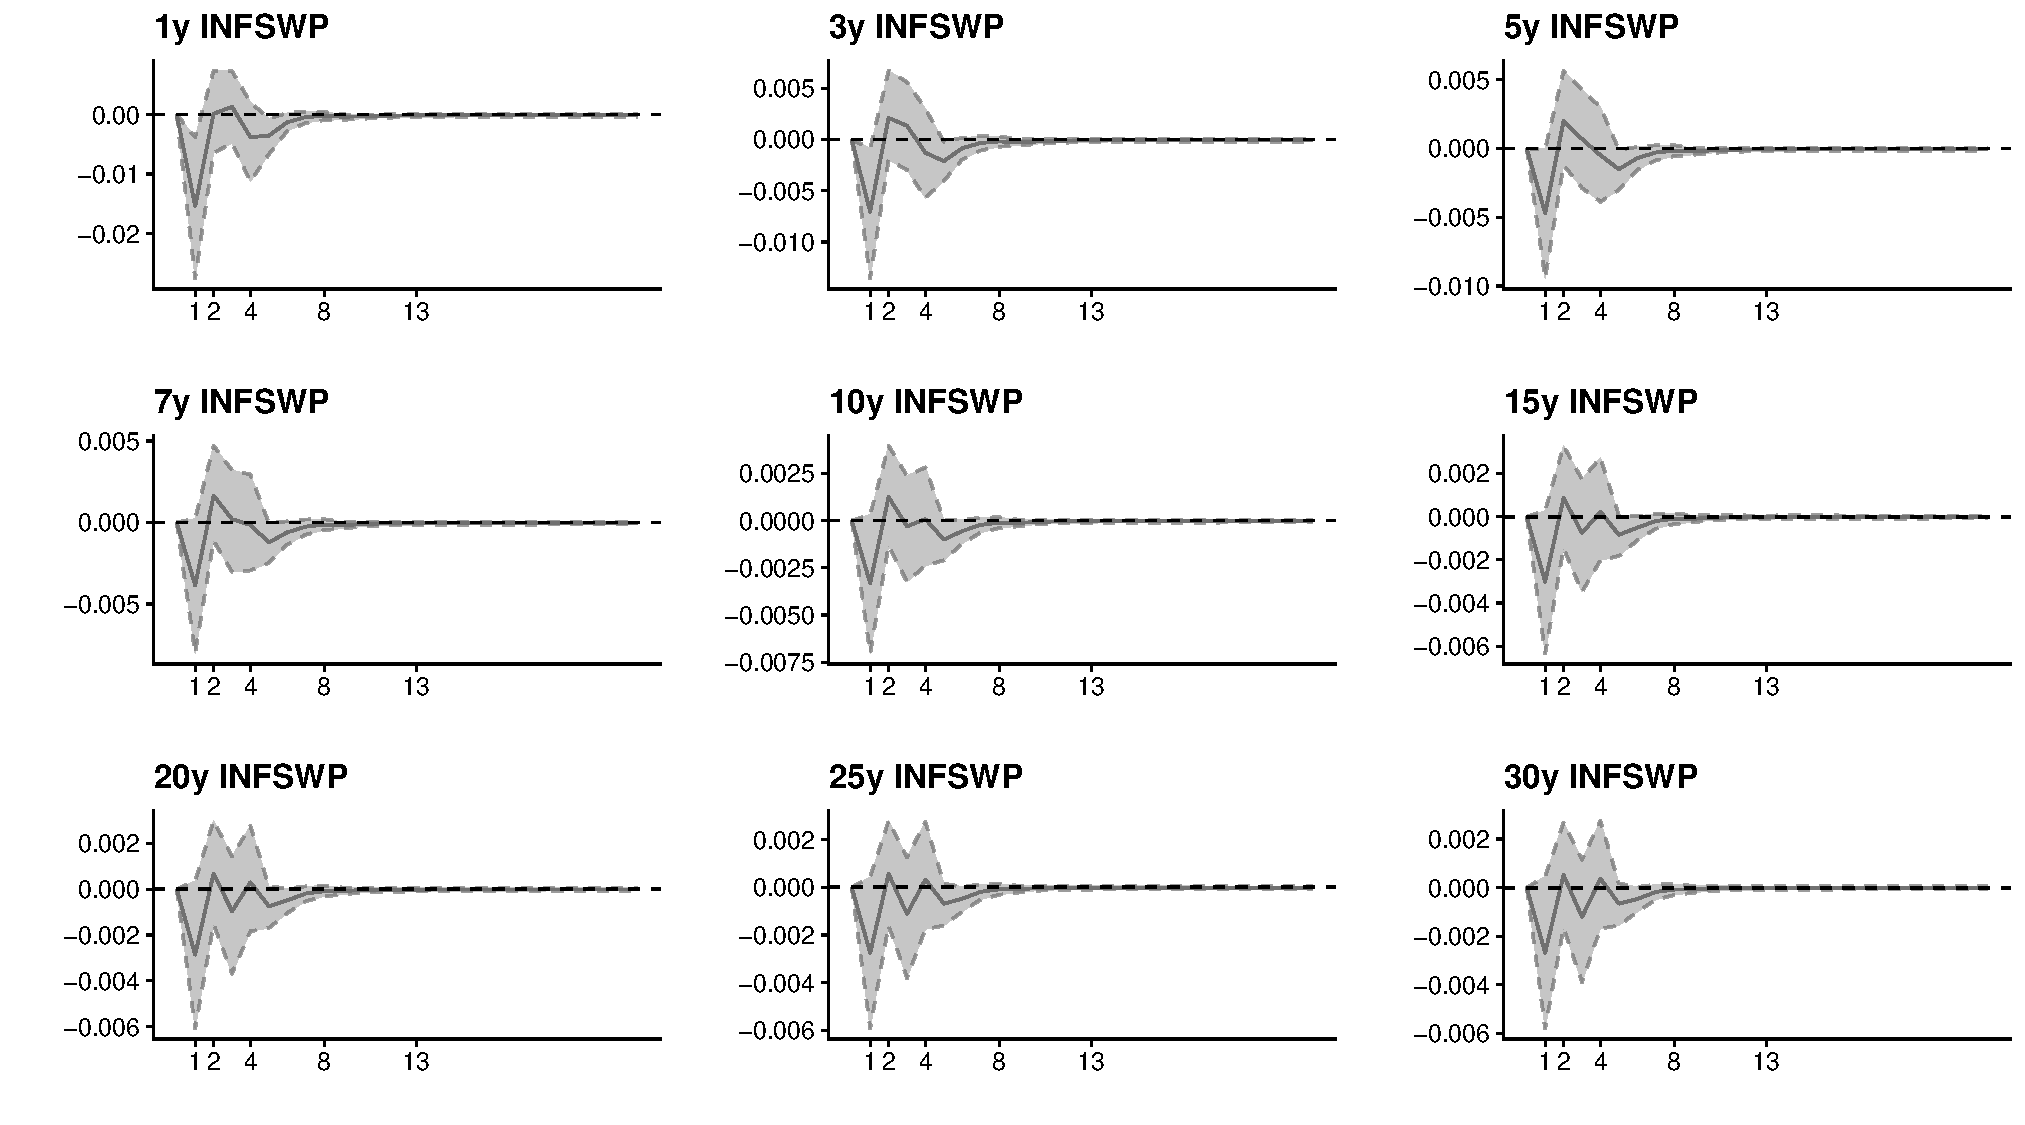
\includegraphics[width= 0.7\textwidth]{images_updated/DIFF_EA_Motto/IRF_INFSWP_D_SLCT.pdf}
\end{minipage}
\caption*{\footnotesize \textit{Notes:} Responses of inflation-linked swap rates to a contractionary EA monetary policy shock conditional on a restrictive US stance (95\% percentile of the threshold, red) and an expansionary US stance (5\% percentile, blue); panel (b) shows the difference (restrictive minus expansionary). The horizontal axis indicates weeks after the shock; shaded areas denote the 68\% posterior credible set.}
\end{figure}

\begin{figure}[!htpb]
\caption{Impulse responses of a restrictive EA monetary policy shock for selected\textit{ real rates}.}\label{fig:IRFreal}
\begin{minipage}{\textwidth}
\centering
a) Responses for two scenarios of US monetary policy
\end{minipage}
\begin{minipage}{\textwidth}
\centering
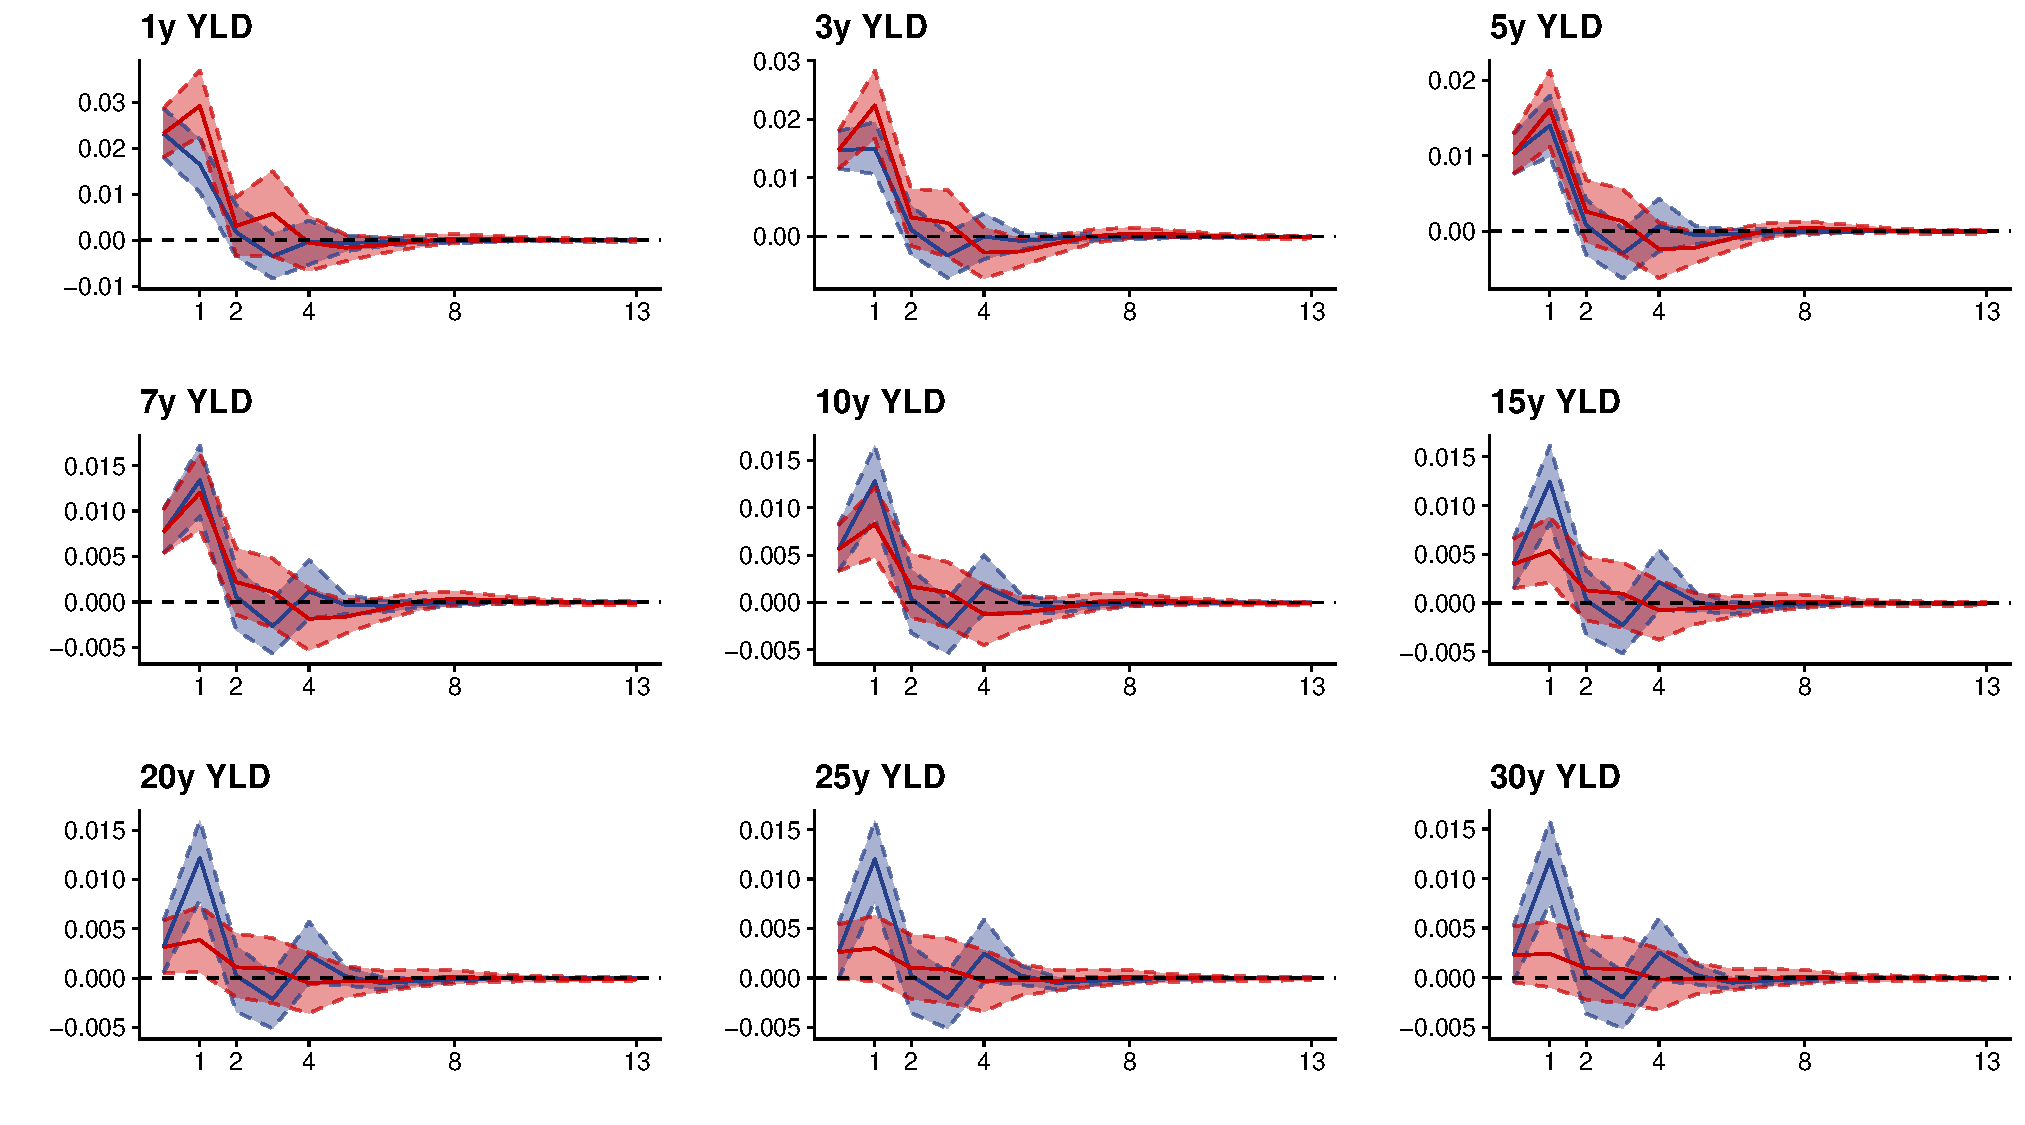
\includegraphics[width= 0.7\textwidth]{images_updated/DIFF_EA_real_Motto/IRF_YLDS_LH_SLCT.pdf}
\end{minipage}
\begin{minipage}{\textwidth}
\centering
b) Difference in responses
\end{minipage}
\begin{minipage}{1\textwidth}
\centering
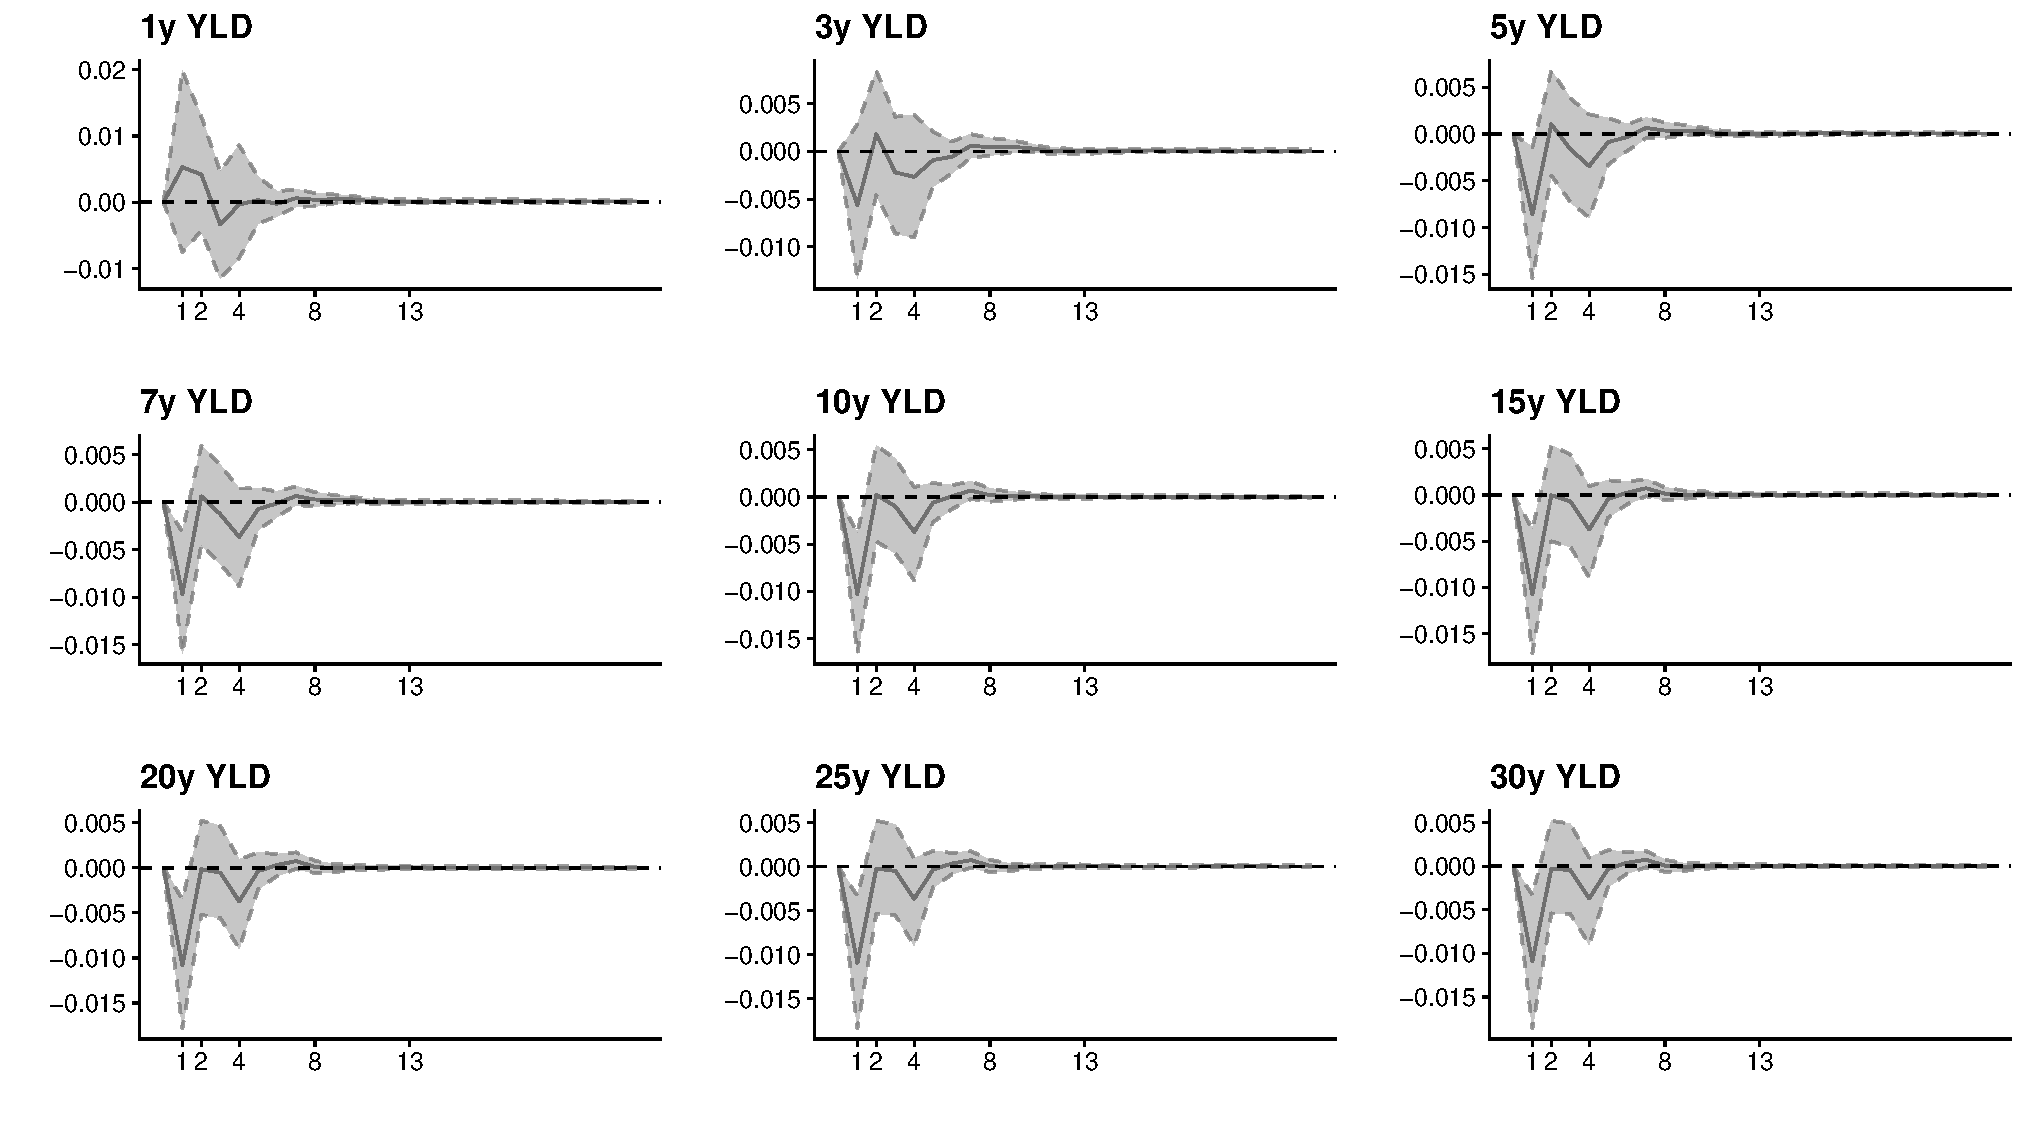
\includegraphics[width= 0.7\textwidth]{images_updated/DIFF_EA_real_Motto/IRF_YLDS_D_SLCT.pdf}
\end{minipage}
\caption*{\footnotesize \textit{Notes:} Responses of real yields (computed draw-wise as the nominal yield response minus the corresponding inflation swap response) to a contractionary EA monetary policy shock, conditional on a restrictive US stance (95\% percentile, red) and an expansionary US stance (5\% percentile, blue); panel (b) shows the difference. Shaded areas denote the 68\% posterior credible set.}
\end{figure}

\begin{figure}[!htpb]
\caption{Cumulated (level) responses of government bond yields to a restrictive EA monetary policy shock.\label{fig:IRFcum}}
\begin{minipage}{\textwidth}
\centering
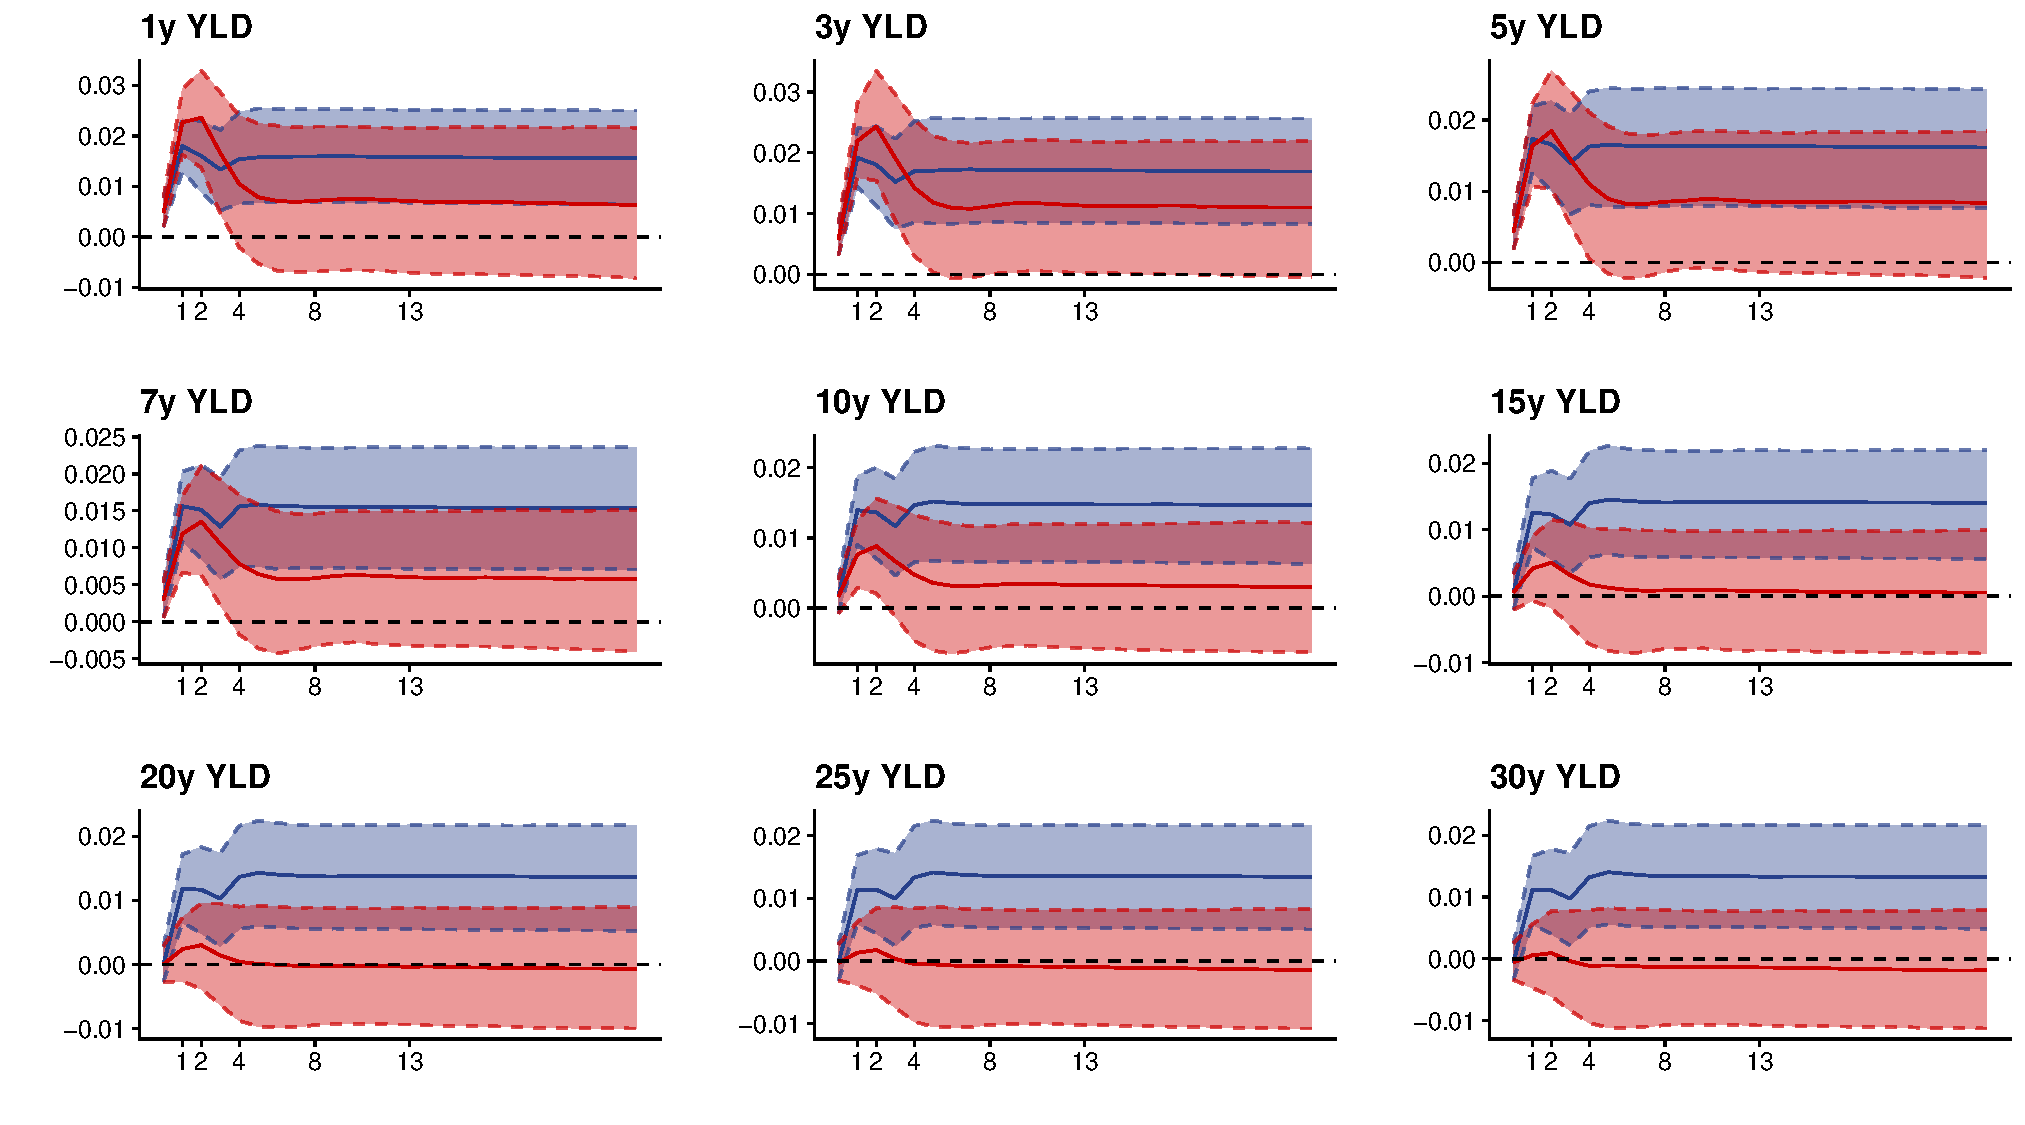
\includegraphics[width=0.85\textwidth]{images_updated/rev/IRF_YLDS_CUM_LH_SLCT.pdf}
\end{minipage}
\caption*{\footnotesize \textit{Notes:} Cumulated impulse responses (implied level effects, in percentage points) under a restrictive (95\% percentile, red) and an expansionary (5\% percentile, blue) US monetary policy stance, over the 26-week horizon. Shaded areas denote the 68\% posterior credible set.}
\end{figure}

% \begin{figure}[!htbp]
% \caption{Peak responses of a restrictive EA monetary policy shock for a set of US monetary policy scenarios.\label{fig:IRFpeaks}}
% \begin{minipage}{\textwidth}
% \centering
% a) Full yield curve
% \end{minipage}
% \begin{minipage}{\textwidth}
% \centering
% 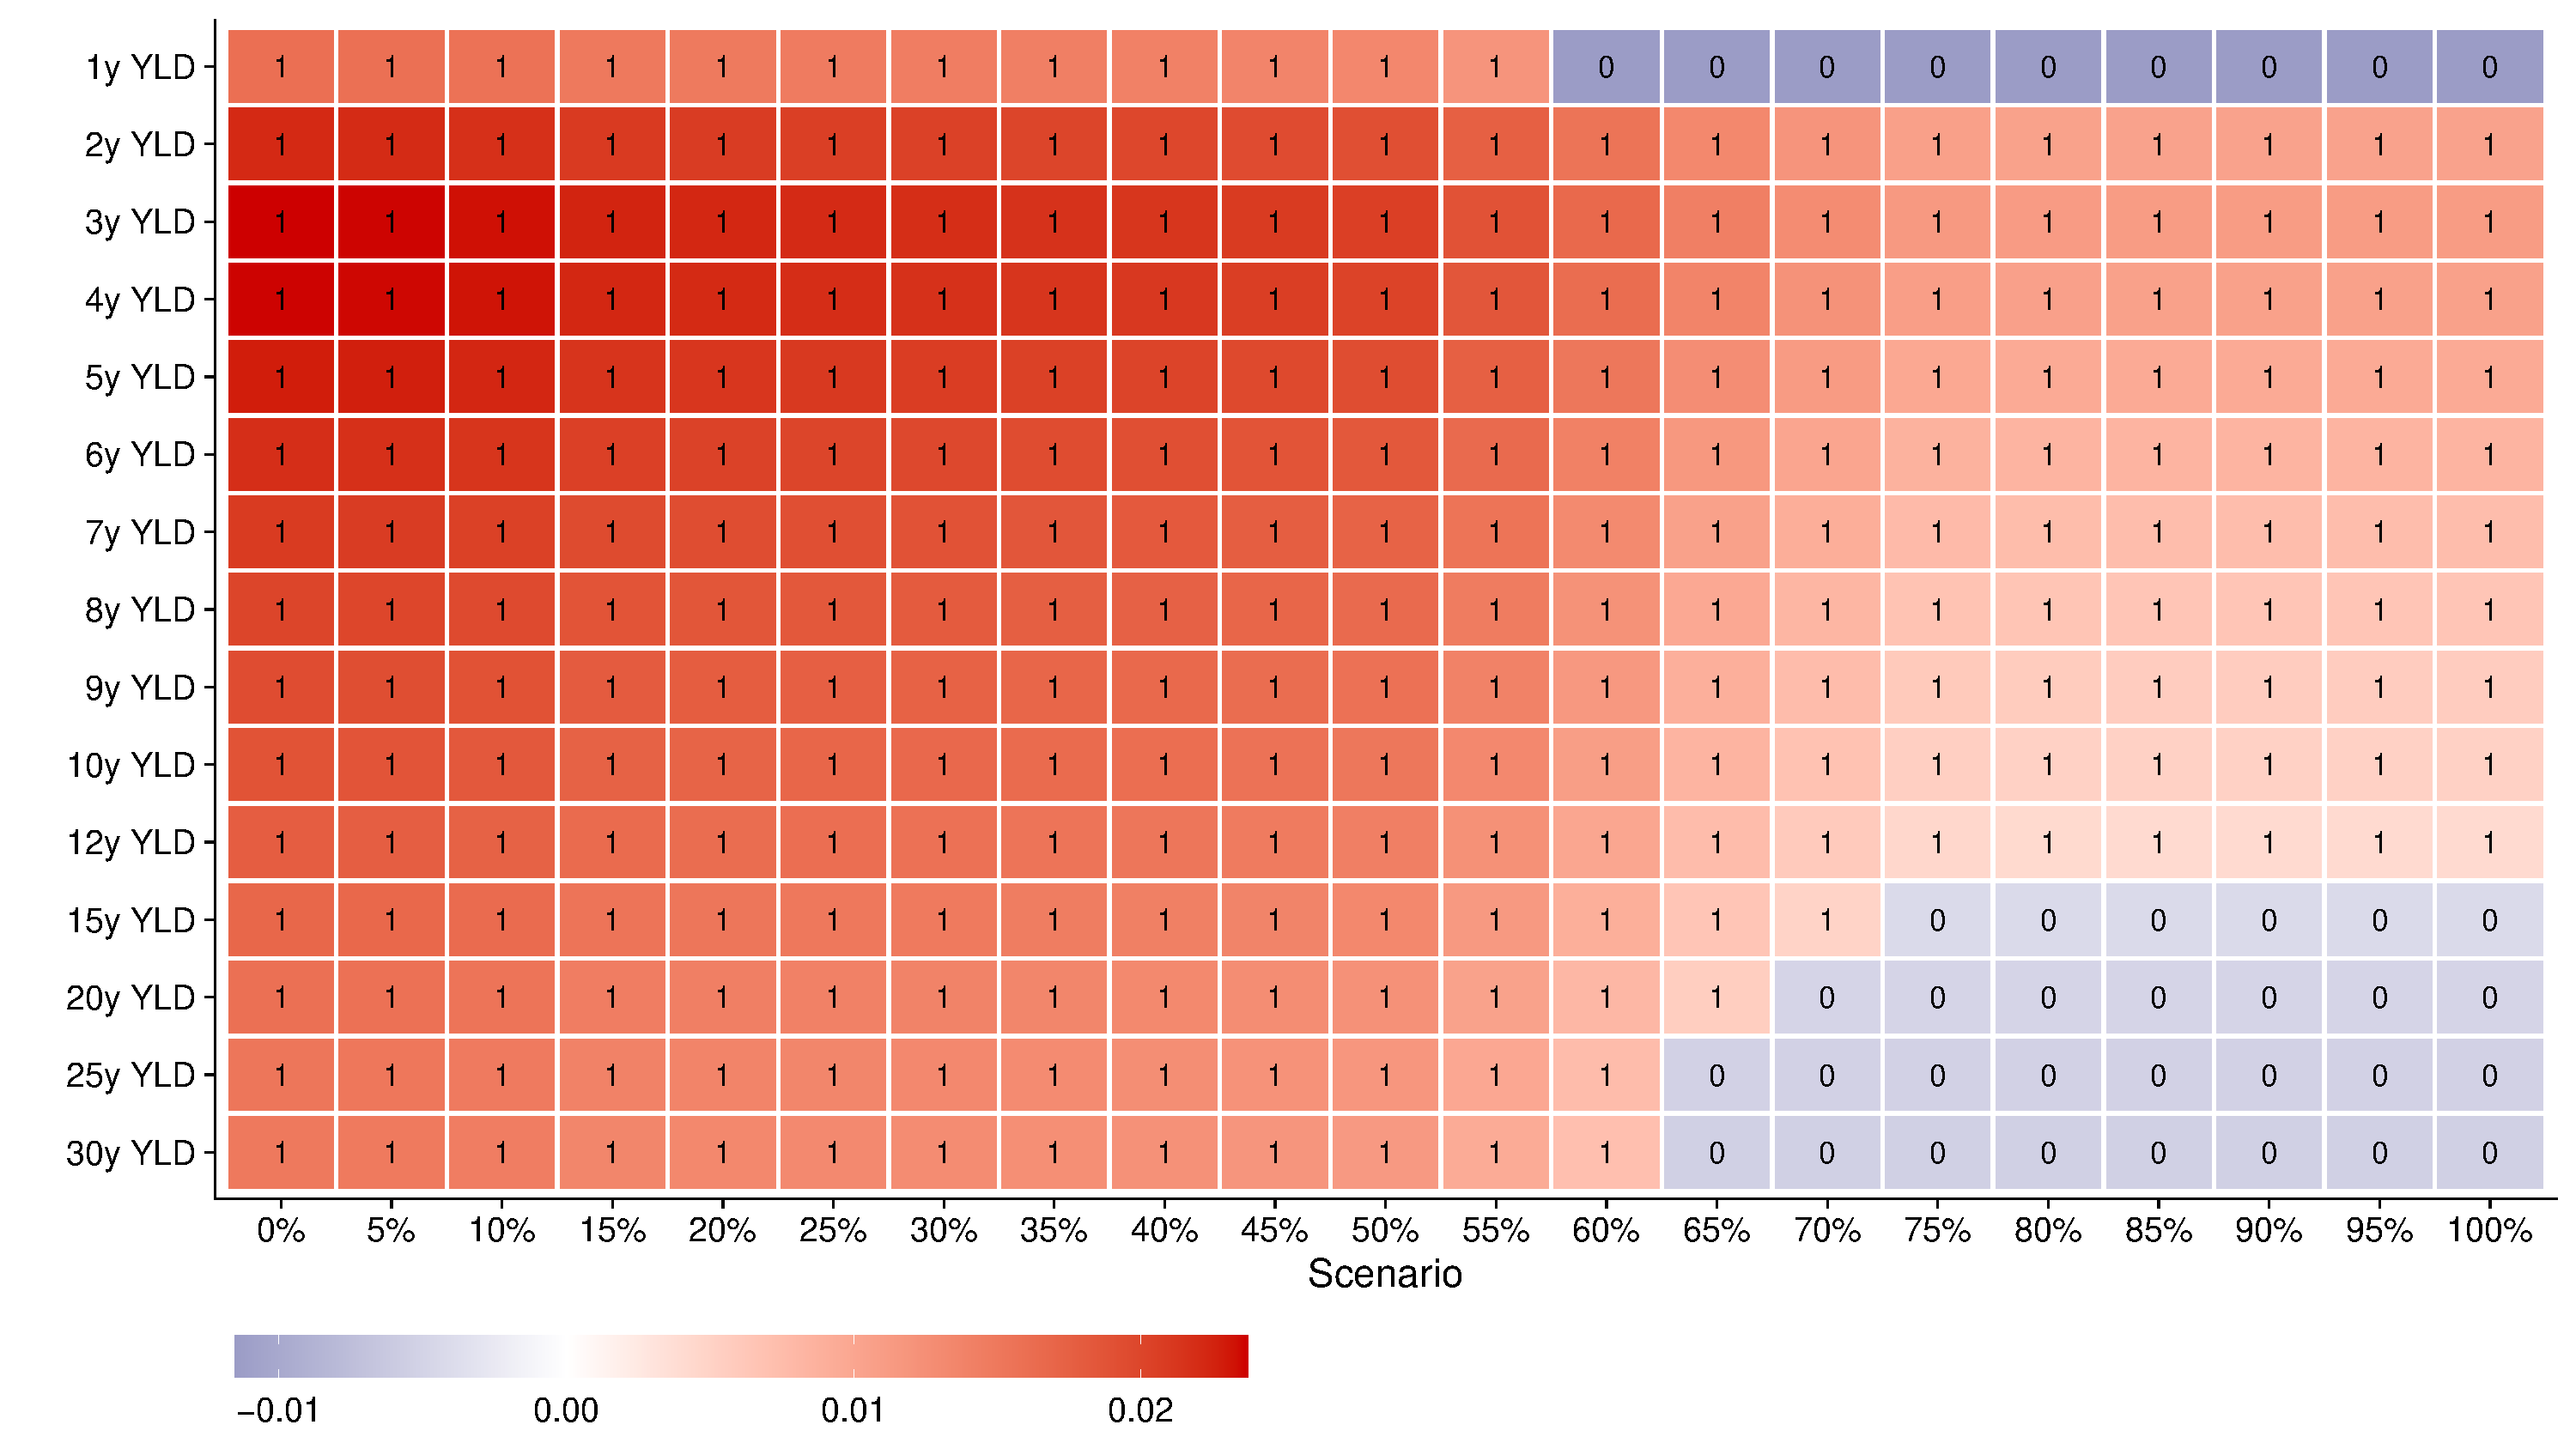
\includegraphics[width= 0.65\textwidth]{images_updated/DIFF_EA_Motto/IRF_YLDS_PEAK.pdf}
% \end{minipage}
% \begin{minipage}{\textwidth}
% \centering
% b) Inflation swaps
% \end{minipage}
% \begin{minipage}{1\textwidth}
% \centering
% 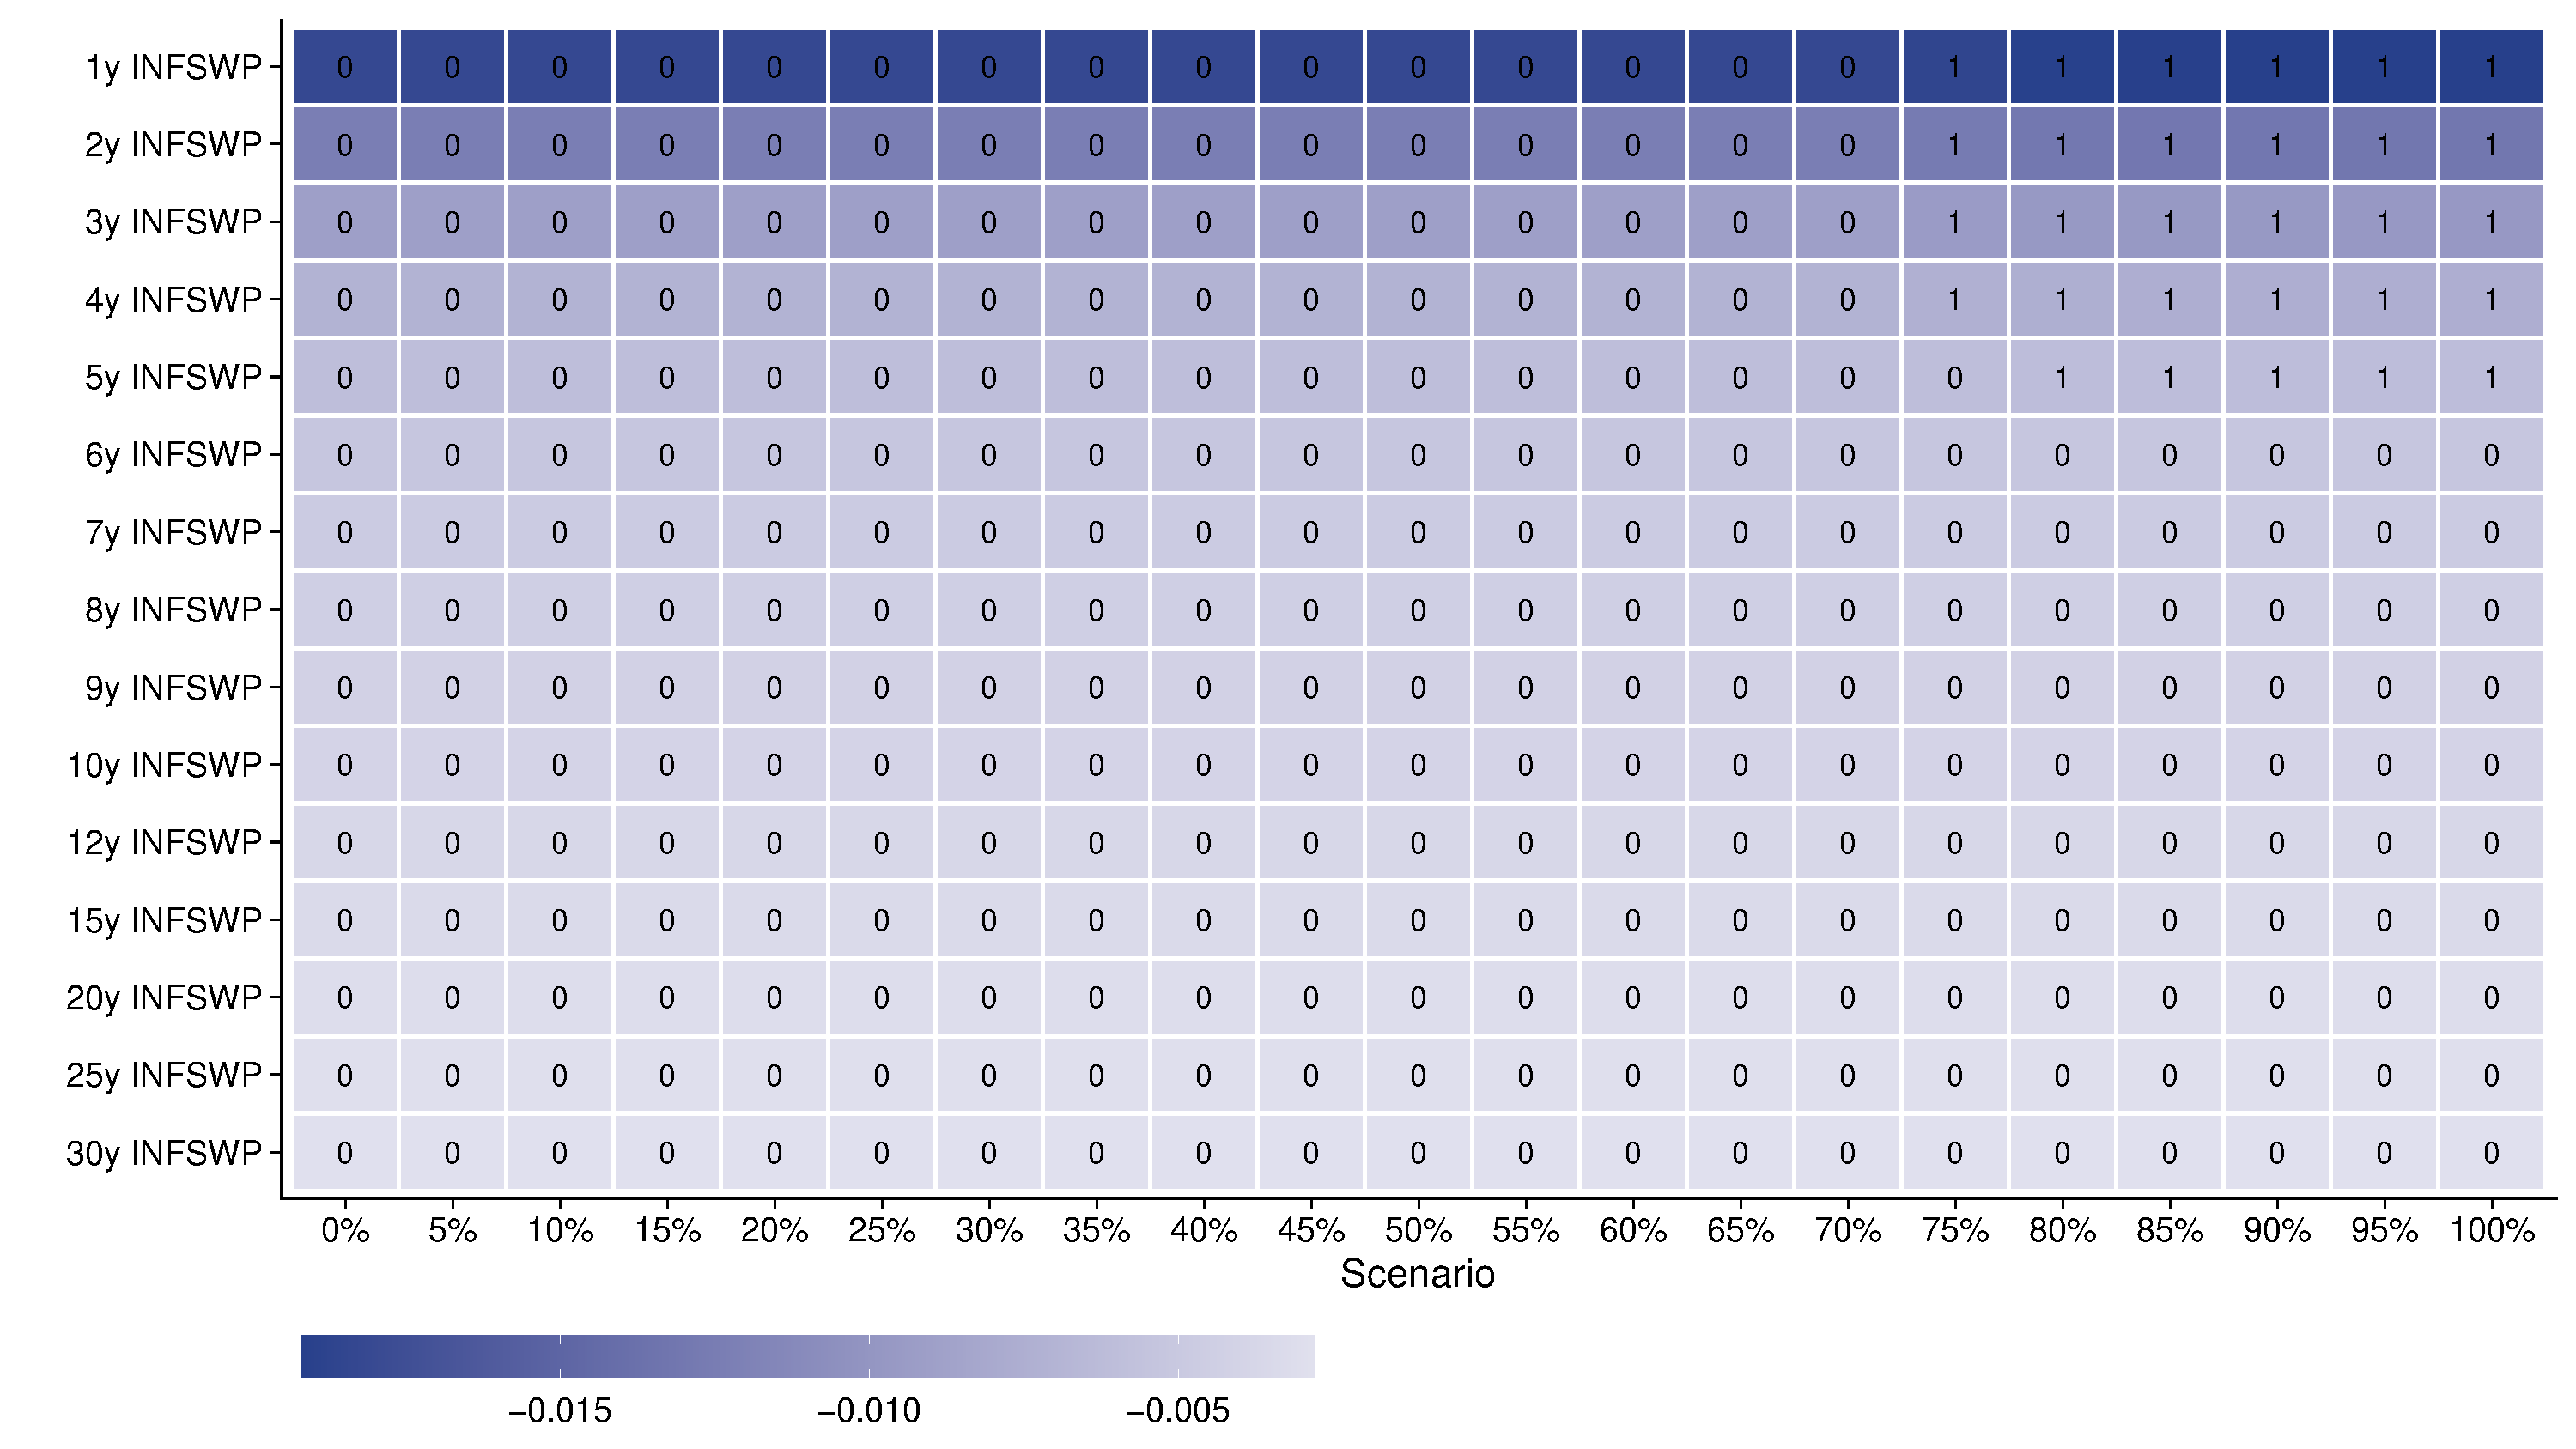
\includegraphics[width= 0.65\textwidth]{images_updated/DIFF_EA_Motto/IRF_INFSWP_PEAK.pdf}
% \end{minipage}
% \begin{minipage}{\textwidth}
% \centering
% c) Real rates (difference between government bond yields and inflation swaps)
% \end{minipage}
% \begin{minipage}{1\textwidth}
% \centering
% 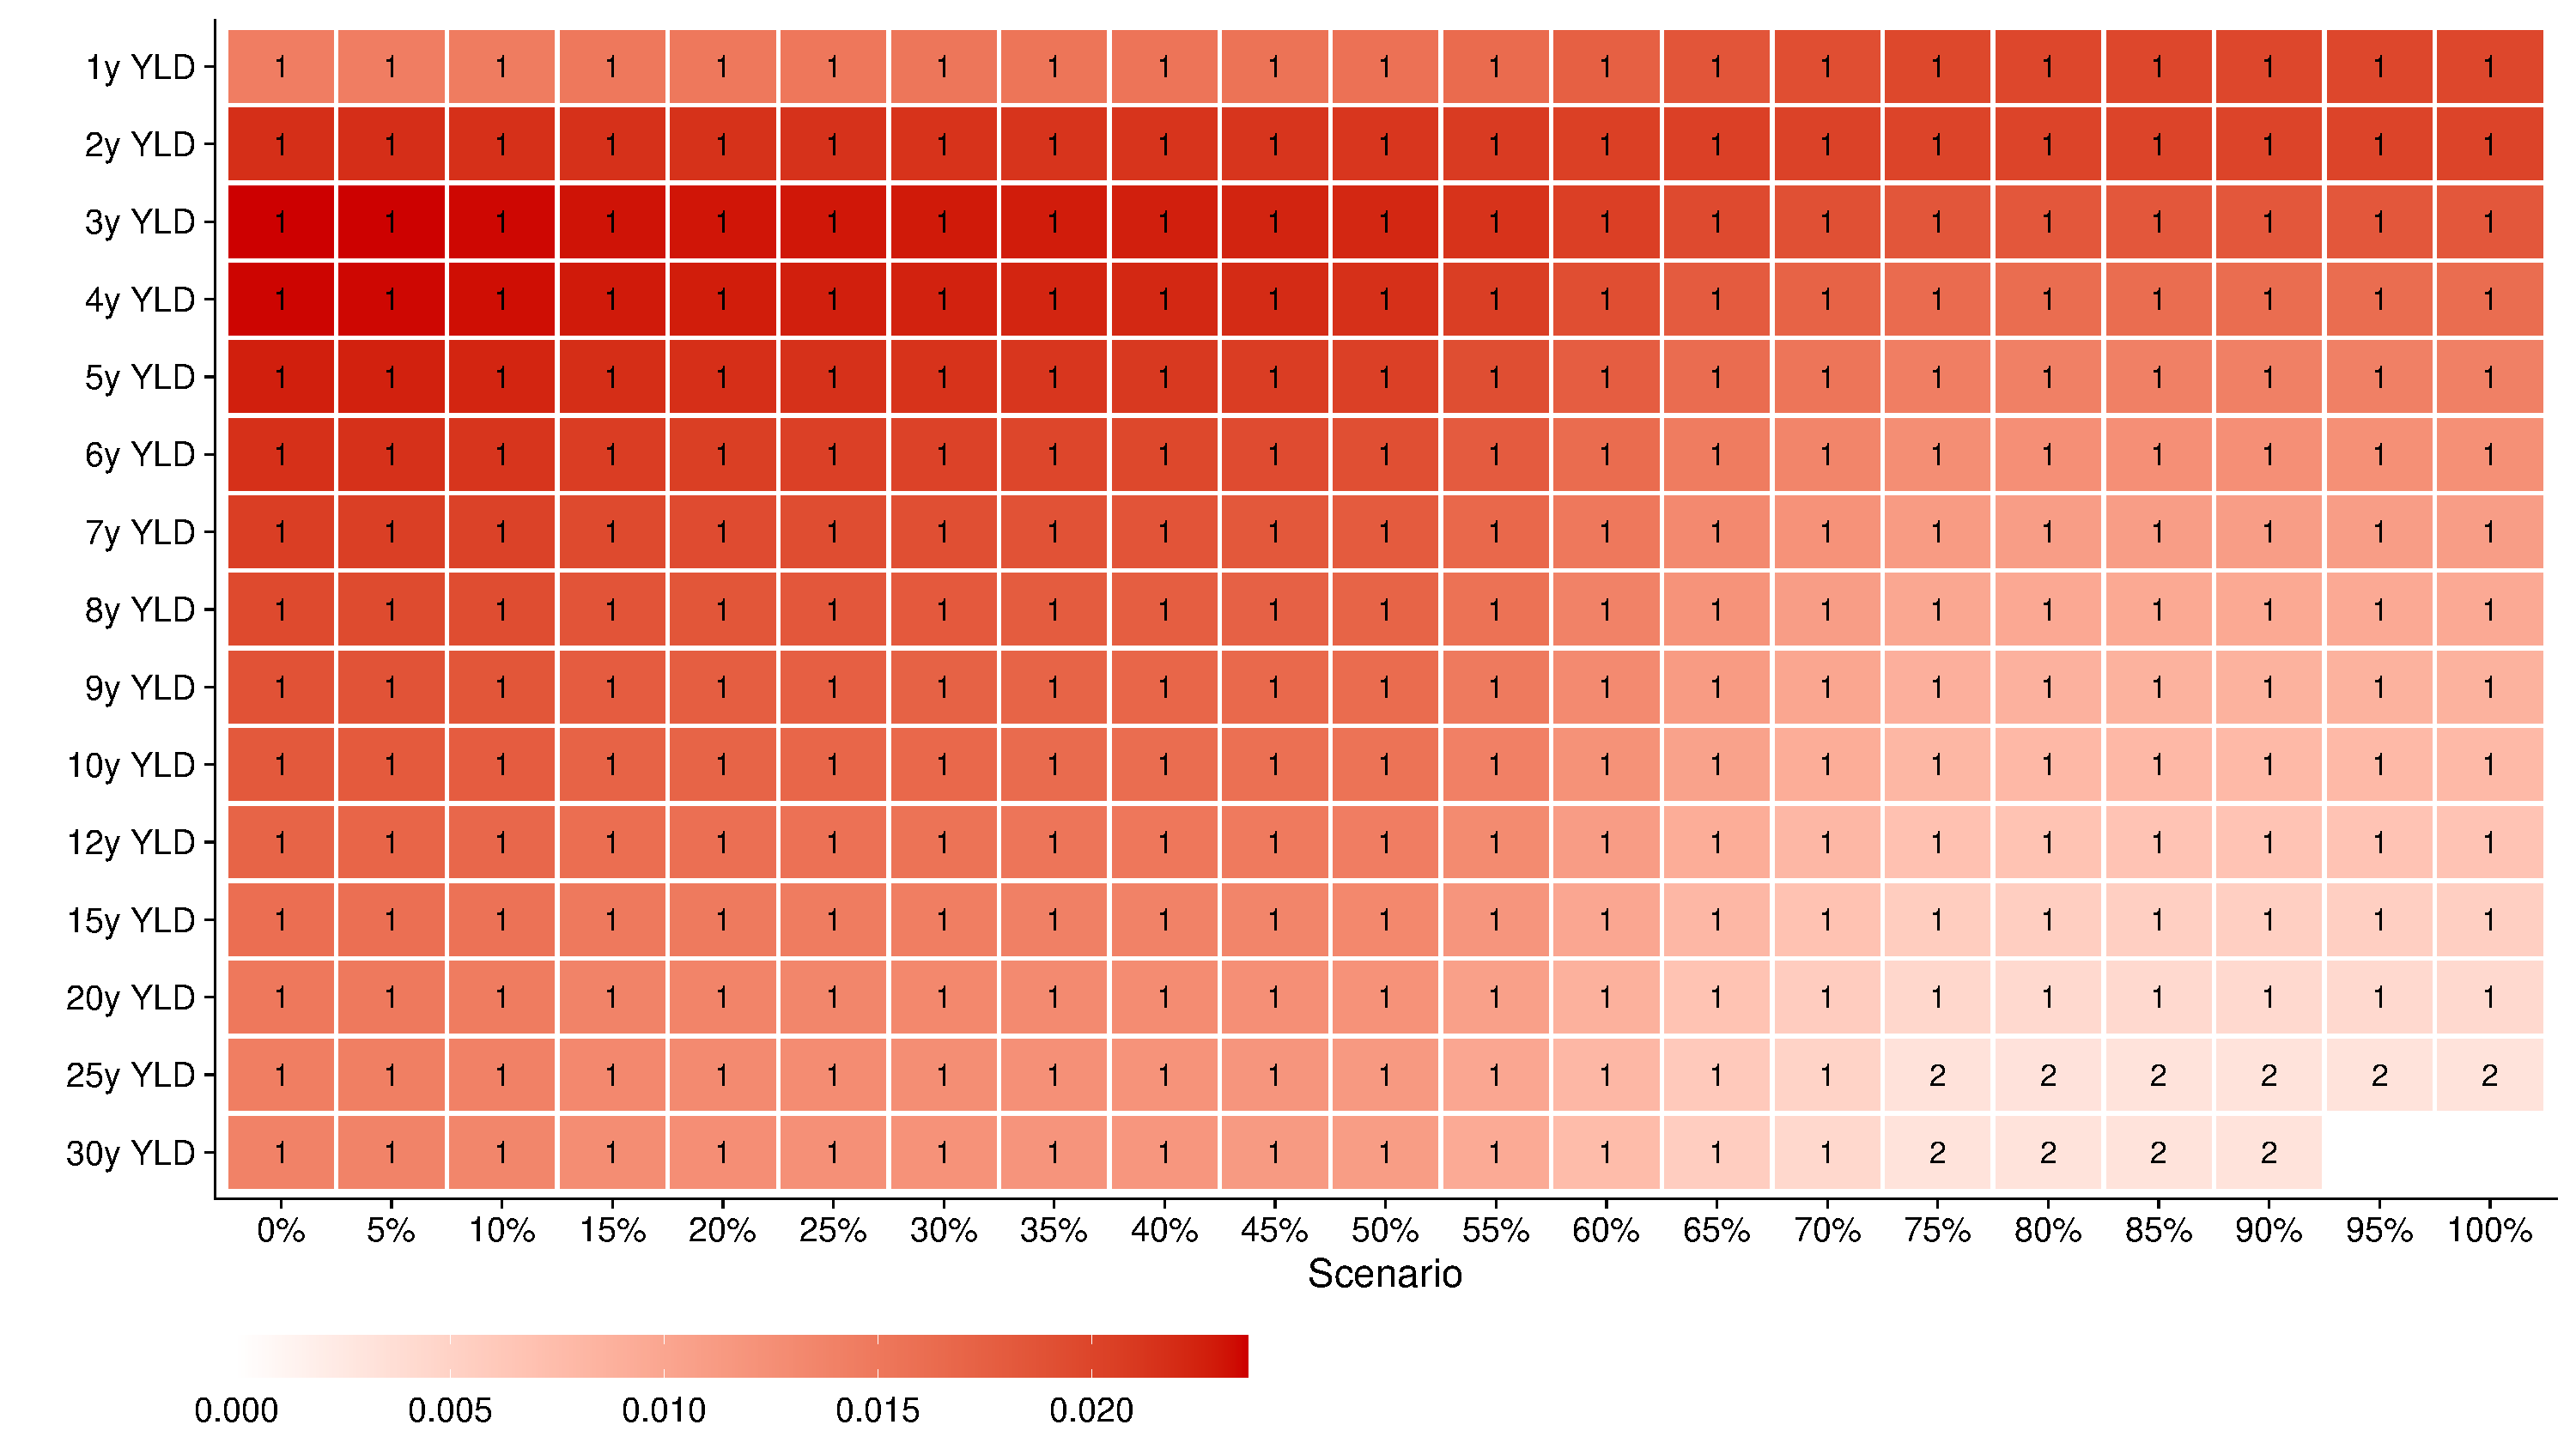
\includegraphics[width= 0.65\textwidth]{images_updated/DIFF_EA_real_Motto/IRF_YLDS_PEAK.pdf}
% \end{minipage}
% \begin{minipage}{\textwidth}
% \centering
% d) Other macrofincancial quantities
% \end{minipage}
% \begin{minipage}{1\textwidth}
% \centering
% 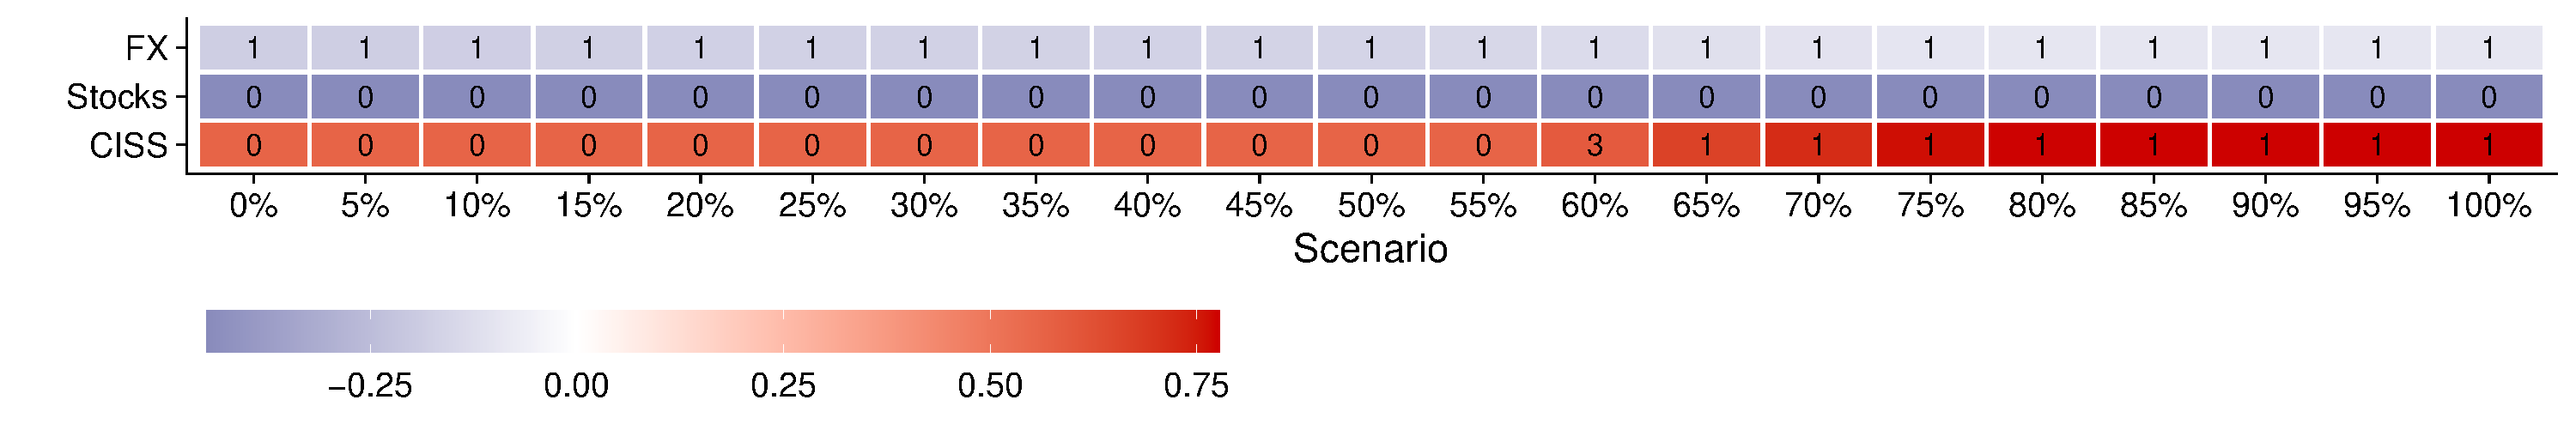
\includegraphics[width= 0.65\textwidth]{images_updated/DIFF_EA_Motto/IRF_OTHERS_PEAK.pdf}
% \end{minipage}
% \caption*{\footnotesize \textit{Notes:} While red (blue) shaded cells indicate significant negative (positive) peak responses, the cell number refers to the week after the shock at which the a significant response peaks. Significance is defined with respect to the $68\%$ credible set.}
% \end{figure}

\clearpage
\section{Robustness Checks}\label{app:rob}
%% Appendix B (Robustness). 


This appendix reports the robustness exercise summarized in \autoref{sec:results_rob} in full. We vary, one at a time, each of the four ingredients that could in principle change the rotation rather than reveal it: the measure of the Fed's stance, which determines the regime allocation; the measure of the euro area policy surprise, which determines the impulse; and the two transition parameters. \autoref{tab:robspecs} lists the resulting specifications, the share of weeks it assigns to the restrictive regime, and the correlation of its posterior
median impulse responses with the baseline.

\textcolor{blue}{comment out the code name column. remove the steepness prior row.}
\begin{table}[!htpb]
\caption{Robustness specifications.\label{tab:robspecs}}
\centering \footnotesize
\resizebox{\textwidth}{!}{% generated by Results/diagnostics/make_robustness_tables.R
% 2026-07-27 (by hand): code-name column removed; "neutral cut" renamed "neutral stance".
% Code names retained as end-of-row comments for the replication package.
\begin{tabular}{lrr}
\hline\hline
Change relative to the baseline & Restrictive & Corr. with \\
 & share & baseline IRFs \\
\hline
Baseline: $DFF-r^\ast$ stance, four-factor surprise, $\mu=0$, $\rho\sim G(4000,1000)$ & 41.0\% & 1.000 \\ % main
Stance replaced by the Krippner shadow short rate less $r^\ast$ & 41.0\% & 0.973 \\ % ssr
Surprise replaced by \cite{jarocinski2020deconstructing} median-rotation shocks & 41.0\% & 0.769 \\ % jk
Neutral stance lowered to $-0.50$ pp & 54.6\% & 0.994 \\ % zlo50
Neutral stance lowered to $-0.25$ pp & 46.6\% & 0.998 \\ % zlo25
Neutral stance raised to $+0.25$ pp & 37.7\% & 0.999 \\ % zhi25
Neutral stance raised to $+0.50$ pp & 34.8\% & 0.994 \\ % zhi50
Steepness prior centred at $7$ instead of $4$ & 41.0\% & 0.998 \\ % rho7
\hline\hline
\end{tabular}
}
\caption*{\footnotesize \textit{Notes:} Each specification alters exactly one ingredient of the baseline and leaves the remainder unchanged. The restrictive share is the fraction of weeks with posterior mean $S_t > 0.5$. The final column is the correlation between the posterior median yield responses of the specification and those of the baseline, taken across all maturities, stance percentiles and horizons. Note that the correlation is not directly comparable for \texttt{jk}, whose surprise series is a different object with a different scale.}
\end{table}

\autoref{tab:robgap} reports the state dependence itself: the difference between the response at the fifth and at the ninety-fifth percentile of the stance, and the posterior probability that this difference is positive. The sign and the maturity profile are common to every specification. The
gap is negative at one year, indistinguishable from zero, and positive
and increasing in maturity from ten years out, where the posterior probability of a positive gap is at least $0.92$ in seven of the eight specifications and $0.82$ in the eighth. Its magnitude, however, varies by a factor of more than three across specifications, and we accordingly make no claim about the size of the effect in the main text.

\begin{table}[!htpb]
\caption{The state-dependence gap across specifications.\label{tab:robgap}}
\centering \footnotesize
\resizebox{\textwidth}{!}{% generated by Results/diagnostics/make_robustness_tables.R -- do not edit by hand
\begin{tabular}{lrrrrrrrr}
\hline\hline
Maturity & Baseline & SSR $-r^\ast$ & JK shocks & $\mu=-0.50$ & $\mu=-0.25$ & $\mu=+0.25$ & $\mu=+0.50$ & $\rho$ prior $7$ \\
\hline
\multicolumn{9}{l}{\textit{1 year}} \\
 \quad median gap & -0.46 & -0.80 & -0.50 & -0.58 & -0.57 & -0.32 & -0.09 & -0.52 \\
 \quad $P(\text{gap}>0)$ & 0.26 & 0.12 & 0.27 & 0.23 & 0.23 & 0.33 & 0.44 & 0.21 \\
\multicolumn{9}{l}{\textit{3 years}} \\
 \quad median gap & -0.28 & -1.15 & -0.02 & -0.25 & -0.31 & -0.16 & 0.02 & -0.45 \\
 \quad $P(\text{gap}>0)$ & 0.36 & 0.07 & 0.49 & 0.39 & 0.34 & 0.42 & 0.52 & 0.26 \\
\multicolumn{9}{l}{\textit{5 years}} \\
 \quad median gap & 0.10 & -0.75 & 0.17 & 0.18 & 0.11 & 0.16 & 0.25 & -0.06 \\
 \quad $P(\text{gap}>0)$ & 0.55 & 0.15 & 0.64 & 0.59 & 0.56 & 0.59 & 0.64 & 0.46 \\
\multicolumn{9}{l}{\textit{10 years}} \\
 \quad median gap & 0.63 & 0.05 & 0.36 & 0.76 & 0.68 & 0.58 & 0.53 & 0.56 \\
 \quad $P(\text{gap}>0)$ & 0.85 & 0.53 & 0.77 & 0.85 & 0.85 & 0.84 & 0.82 & 0.85 \\
\multicolumn{9}{l}{\textit{15 years}} \\
 \quad median gap & 0.85 & 0.37 & 0.43 & 0.99 & 0.91 & 0.76 & 0.65 & 0.83 \\
 \quad $P(\text{gap}>0)$ & 0.93 & 0.75 & 0.80 & 0.91 & 0.92 & 0.91 & 0.87 & 0.94 \\
\multicolumn{9}{l}{\textit{30 years}} \\
 \quad median gap & 1.08 & 0.71 & 0.48 & 1.22 & 1.16 & 0.96 & 0.79 & 1.08 \\
 \quad $P(\text{gap}>0)$ & 0.97 & 0.89 & 0.81 & 0.96 & 0.97 & 0.95 & 0.90 & 0.98 \\
\hline\hline
\end{tabular}
}
\caption*{\footnotesize \textit{Notes:} The gap is the one-week-ahead response at the fifth percentile of the Fed's stance less the response at the ninety-fifth percentile, in basis points per one standard deviation euro area surprise, computed draw by draw. $P(\text{gap}>0)$ is the share of posterior draws in which the gap is positive. Because the surprise is standardized within each specification, magnitudes are comparable across all columns except \texttt{jk}, whose underlying series has a standard deviation of $3.5$ rather than $5.7$ basis points; for that column the sign and the maturity profile are informative but the level is not.}
\end{table}

\autoref{tab:robrot} states the rotation directly. Panel A records, for each maturity, the highest percentile of the Fed's stance at which the response is still significantly positive; reading down a column traces the rotation, since a response that survives at every percentile at short maturities but fails beyond the fiftieth or sixtieth at long maturities is precisely a curve that pivots rather than shifts. Panel B records the lowest percentile at which the response has become significantly
negative. The distinction matters: an unsigned test that merely asked whether the credible band excludes zero would treat a significantly negative long-end response as though the response were robustly present, when in fact it is the strongest form of the rotation. In three specifications the thirty-year response does turn significantly negative once the Fed is sufficiently restrictive.

\textcolor{blue}{remove panel B as it is everywhere the same result. just mention one sentence in the paragraph above}
\begin{table}[!htpb]
\caption{The rotation: signed significance frontier.\label{tab:robrot}}
\centering \footnotesize
\resizebox{\textwidth}{!}{% generated by Results/diagnostics/make_robustness_tables.R
% 2026-07-27 (by hand): Panel B (negative frontier) removed -- it is "--" for every
% specification at every maturity under seed 1002; the point is now made in one sentence
% in the appendix text.
\begin{tabular}{lrrrrrrrr}
\hline\hline
Maturity & Baseline & SSR $-r^\ast$ & JK shocks & $\mu=-0.50$ & $\mu=-0.25$ & $\mu=+0.25$ & $\mu=+0.50$ & $\rho$ prior $7$ \\
\hline
1 year & 100 & 100 & 100 & 100 & 100 & 100 & 100 & 100 \\
3 years & 100 & 100 & 100 & 100 & 100 & 100 & 100 & 100 \\
5 years & 100 & 100 & 100 & 100 & 100 & 100 & 100 & 100 \\
10 years & 100 & 100 & 70 & 100 & 100 & 100 & 100 & 100 \\
15 years & 100 & 100 & 60 & 100 & 100 & 100 & 100 & 100 \\
30 years & 65 & 70 & 55 & 65 & 65 & 70 & 70 & 60 \\
\hline\hline
\end{tabular}
}
\caption*{\footnotesize \textit{Notes:} Entries are percentiles of the Fed's stance distribution.
Panel~A gives the highest percentile at which the sixteenth posterior quantile of the response is
still above zero, Panel~B the lowest percentile at which the eighty-fourth quantile has fallen
below zero. ``--'' indicates that the condition is never met. A value of $100$ in Panel~A means
the response remains significantly positive across the entire stance distribution.}
\end{table}

\textcolor{blue}{cut is missleading. work with neutral stance and change everything accordingly here}
Finally, \autoref{fig:zetafrontier} isolates the dependence on the calibrated neutral stance. Lowering the neutral stance confines the accommodative state to more deeply accommodative weeks and widens the estimated gap; raising it has
the opposite effect. What the figure also shows, however, is that the credible band lies entirely above zero over the whole range considered, at both maturities: the existence of the state dependence does not turn on where the boundary is placed, only its measured size does.

\begin{figure}[!htpb]
\caption{The state-dependence gap as a function of the calibrated neutral
stance.\label{fig:zetafrontier}}
\centering
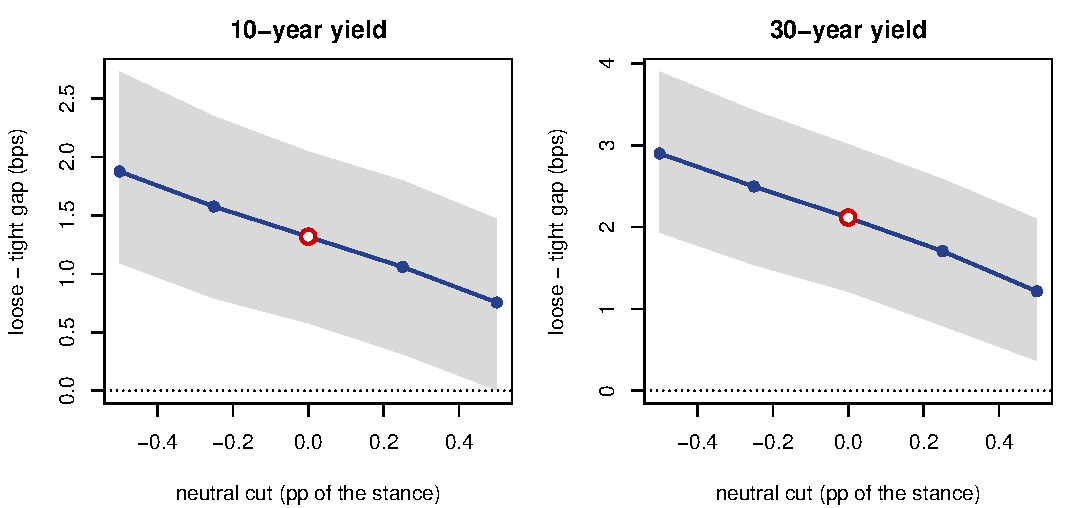
\includegraphics[width=\textwidth]{images_updated/rob/zeta_frontier.pdf}
\caption*{\footnotesize \textit{Notes:} Posterior median (solid line) and $68\%$ credible band
(shaded) of the loose-minus-tight gap in the one-week-ahead yield response, plotted against the
calibrated neutral cut $\mu$ in percentage points of the Fed's stance. The open red circle marks
the baseline calibration $\mu=0$, at which the restrictive regime comprises $41.0\%$ of weeks; the
end points $\mu=\mp0.50$ correspond to $54.6\%$ and $34.8\%$ respectively. Left panel: ten-year
yield. Right panel: thirty-year yield.}
\end{figure}



\clearpage
\section{Technical appendix}\label{app:B}
\subsection{Prior set-up}\label{app:prior}
For the prior setup, we closely follow \cite{hauzenberger2020effectiveness}. Our priors are designed to provide sufficient regularization of the VAR coefficients to reduce estimation uncertainty. On the VAR coefficients, we therefore apply a Horseshoe (HS) prior \citep{carvalho2010horseshoe}, which belongs to the class of global-local shrinkage techniques. To outline the mechanism of this prior, it proves useful to collect the state-specific coefficients in an $M \times N$-dimensional matrix $\bm A_k = (\bm c_k, \bm \gamma_k, \bm A_kp, \dots, \bm A_kP)$, for $k = \{0, 1\}$ and $p=1,...,P$. In the following, let $\bm a_k = \text{vec}(\bm A_k)$ be a $K (= NM)$-dimensional vector, then, for $k = \{0, 1\}$, then the hierarchical HS prior on the $j$th ($j = 1, \dots, K)$ state-specific coefficients is as follows:
\begin{equation*}
a_{kj} \sim \mathcal{N}(0, \tau_k \lambda_{kj}), \quad \sqrt{\tau_k} \sim \mathcal{C}^+(0,1) \quad \text{and} \quad \sqrt{\lambda_{kj}} \sim \mathcal{C}^+(0,1).   
\end{equation*}
Here, a global component $\tau_k$ pushes all coefficients in $\bm a_k$ toward zero (i.e., the prior mean), while local scaling parameters $\lambda_{kj}$ are regime- and covariate-specific, providing sufficient flexibility.  Both hyperparameters $\sqrt{\tau_{k}}$ and $\sqrt{\lambda_{kj}}$ follow a half-Cauchy distribution denoted by $\mathcal{C}^+$. This prior is able to introduce sufficient sparsity via the global shrinkage component in a highly parameterized model that would otherwise be prone to overfitting. The local scales still allow for the detection of important individual covariates by mitigating the potential (over)shrinkage of the global parameter. 

The prior specification on the variance-covariance $\bm \Sigma$ is standard. Here, $\bm \Sigma$ follows an inverted Wishart distribution: 
\begin{equation*}
    \bm \Sigma \sim \mathcal{IW}(d_0, \bm D_0), 
\end{equation*}
with the scalar $d_0$ denoting the prior degrees of freedom and the $M\times M$-dimensional matrix $\bm D_0$ referring to the prior scaling. In the empirical application, we specify $d_0 = M+2$ and $\bm D_0 = 0.01 \bm I_M$. This choice ensures that the prior is proper, but still weakly informative.

To complete our proposed setup, we also need to specify priors on the hyperparameters $\mu$ and $\rho$, which define the transition between the two regimes. The threshold parameter $\mu$ follows a weakly informative Uniform distribution:
\begin{equation*}
    \rev{\mu \sim \mathcal{U}\left(\bar{z}^* - 0.5,\; \bar{z}^* + 0.5\right),}
\end{equation*}
\rev{with the prior support centered on the sample mean $\bar z^*$ of the (standardised) signal variable, i.e., spanning half a standard deviation on either side of the mean. Widening the support to the full range of $z_t^*$ leaves the posterior of $\mu$ virtually unchanged.}
On the speed of adjustment parameter $\rho$ we impose a Gamma prior: 
\begin{equation*}
    \rho \sim \mathcal{G}(s_0, s_1), 
\end{equation*}
with the hyperparameters \rev{$s_0=4/0.001$ and $s_1=1/0.001$ (prior mean $4$, prior standard deviation $0.06$)} chosen such that the transition between the two states occurs relatively fast. This informative choice ensures a sensible state allocation and a clear separation between the two regimes, one characterized by an expansionary US monetary policy and the other characterized by a restrictive stance (see also \autoref{fig:stallo} for the estimated state allocation). \rev{Centering the prior at $7$ instead of $4$ leaves the state allocation and all impulse responses virtually unchanged; the transition speed is deliberately calibrated, as the likelihood is uninformative about $\rho$.}

\subsection{Posterior quantities and sampling algorithm}\label{app:mcmc}
Next, we outline the main steps of our Markov Chain Monte Carlo (MCMC) algorithm, which is used to simulate from the full posterior distribution. To obtain the conditional posteriors, we combine the priors with the likelihood of the model, as described in \autoref{eq:STVAR} and \autoref{eq:St}. For most parameters, this leads to well-known conditional distributions, and simulating from them is straightforward. Let the symbol $\bullet$ indicate that we condition on the remaining parameters of the system, then these sampling steps read as follows: 
\begin{enumerate}
    \item For simplicity we collect all VAR coefficients in a $2K$-dimensional vector $\bm a = (\bm a_1', \bm a_0')'$ and define the corresponding $2K$-dimensional vector of predictors $\bm x_t = \left((1, z_t, \bm y_{t-1}', \dots, \bm y_{t-p}')\times S_t,  (1, z_t, \bm y_{t-1}', \dots, \bm y_{t-p}') \times (1-S_t)\right)'$. 
    In what follows, we sample $\bm a$ from a multivariate Gaussian distribution: 
    \begin{equation*}
        \bm a|\bullet \sim \mathcal{N}\left(\bar{\bm a}, \bar{\bm V} \right),
    \end{equation*}
    with $\bar{\bm a}$ denoting the posterior mean and $\bar{\bm V}$ the posterior variance-covariance matrix: 
    \begin{equation*}
    \begin{aligned}
       \bar{\bm V} =& \left(\bm \Sigma^{-1} \otimes \bm X'\bm X + \underline{\bm V}^{-1} \right), \\
       \bar{\bm a} =&  \bar{\bm V}^{-1}  \left(\bm \Sigma^{-1} \otimes \bm X'\text{vec}(\bm Y) \right). \end{aligned}
    \end{equation*}
    Here, $\bm X = (\bm x_1, \dots, \bm x_T)'$ and $\bm Y = (\bm y_1, \dots, \bm y_T)'$ denote the full data matrices and $\underline{\bm V} = \text{diag}\left(\{v_{1j}\}_{j=1}^{K}, \{v_{0j}\}_{j=1}^{K}\right)$, where $v_{kj} = \tau_k \lambda_{kj}$, collects the prior variances of all coefficients on the main diagonal. 
    \item To draw the HS scaling parameters we rely on the following steps, outlined in \cite{makalic2015simple}: 
    \begin{equation*}
    \begin{aligned}
        \tau_k|\bullet &\sim \mathcal{IG}\left(\frac{K + 1}{2}, \frac{1}{\phi_k} + \sum_{j = 1}^{K} \frac{a_{kj}}{2\lambda_{kj}}\right), \\
        \lambda_{kj}|\bullet &\sim \mathcal{IG}\left(1, \frac{1}{\zeta_{kj}}+ \frac{a_{kj}}{2 \tau_k}\right), \\
    \end{aligned} 
    \end{equation*}
    where the two auxiliary variables $\phi_k$ and $\zeta_{kj}$ are also drawn from inverted Gamma distributions: 
    \begin{equation*}
    \begin{aligned}
        \phi_k|\bullet &\sim \mathcal{IG}\left(1,1+\frac{1}{\tau_k} \right), \\
        \zeta_{kj}|\bullet &\sim \mathcal{IG}\left(1,1+\frac{1}{\lambda_{kj}} \right).
    \end{aligned} 
    \end{equation*}
    \item We sample $\bm \Sigma$ from an inverted Wishart distribution: 
    \begin{equation*}
        \bm \Sigma|\bullet \sim \mathcal{IW}(d_1, \bm D_1),
    \end{equation*} 
    with posterior degrees of freedom $d_1 = d_0 + T/2$ and $M \times M$-dimensional posterior scaling matrix $\bm D_1 = \bm D_0 + (\bm Y - \bm X \bm a)'(\bm Y - \bm X \bm a)/2 $.
    \item The parameters of the state transition function are sampled jointly with a Metropolis-within-Gibbs step. The candidate values are sampled from independent Gaussian proposal densities: $\mu^{(*)} \sim \mathcal{N}(\mu^{(s)}, \kappa_{\mu})$ and $\rho^{(*)} \sim \mathcal{N}(\rho^{(s)},  \kappa_{\rho})$, with the candidate value $\mu^{(*)}$ ($\rho^{(*)}$) being centered on the last accepted draw $\mu^{(s)}$ ($\rho^{(s)}$) and featuring a variance $\kappa_{\mu}$ ($\kappa_{\rho}$). The acceptance probability of the proposed values is then given by: 
    \begin{equation*}
        \min \left(1, \frac{\mathcal{L}(\mu^{(*)}, \rho^{(*)}|\bullet) p(\mu^{(*)}, \rho^{(*)})}{\mathcal{L}(\mu^{(s)}, \rho^{(s)}|\bullet) p(\mu^{(s)}, \rho^{(s)})} \right),
    \end{equation*}
    with $\mathcal{L}$ denoting the data likelihood conditional on the proposed values ($\mu^{(*)}, \rho^{(*)}$) and last accepted draw ($\mu^{(s)}, \rho^{(s)}$), while $p(\mu^{(*)}, \rho^{(*)})$ and $p(\mu^{(s)}, \rho^{(s)})$ refer to joint prior distribution evaluated at the proposed values and the last accepted draw.
    \rev{In practice, we evaluate $\mathcal{L}$ exactly (up to a proportionality constant that does not depend on $\mu$ and $\rho$) by whitening the system with the error precision matrix. Let $\bm L$ denote the lower Cholesky factor of $\bm\Sigma^{-1} = \bm L \bm L'$ and let $\bm U(\mu, \rho) = \bm Y - \bm X(\mu, \rho)\, \bm A$ collect the reduced-form residuals implied by the candidate transition parameters. The rows of the transformed residual matrix $\bm U(\mu, \rho)\, \bm L$ are standard Gaussian under the model, so that $\log \mathcal{L}(\mu, \rho \mid \bullet) = -\frac{1}{2}\lVert \bm U(\mu, \rho)\, \bm L \rVert_F^2 + \text{const}$, where $\lVert \cdot \rVert_F$ is the Frobenius norm. This makes the Metropolis acceptance ratio an exact evaluation of the conditional posterior of $(\mu, \rho)$.}\footnote{\rev{Note for revision (not for publication): an earlier implementation whitened with the transposed factor $\bm L'$ instead of $\bm L$, which leaves the transformed residual covariance different from the identity matrix and hence renders the acceptance ratio inexact. Correcting this (code: \texttt{STVAR\_rev\_whitenfix.R}, July 2026) leaves all impulse responses and the state allocation virtually unchanged (posterior-median IRF correlations $\geq 0.997$; regime-path correlation $0.99$), but changes the posterior of $\rho$: under the exact likelihood the posterior of $\rho$ essentially coincides with its informative prior, i.e., the speed of adjustment is pinned down by the prior rather than the likelihood, while $\mu$ remains data-identified. Metropolis acceptance rises from $0.09$ to $0.63$.}}
\end{enumerate}
\rev{We repeat these steps $12,000$ times and discard the initial $2,000$ draws as burn-in, retaining $10,000$ draws for inference. [Note for revision: iteration count and the prior settings for $\rho$ and $\mu$ above have been harmonized with the replication code (previously the text stated $15,000/5,000$ iterations, a $\rho$-prior mean of $7$, and min--max support for $\mu$). A check re-estimating the baseline under the text's former settings leaves all results virtually unchanged: regime-path correlation $0.995$, IRF-median correlations $\geq 0.997$, identical hawk--dove contrast.]}


\end{appendices}

%\appendix




\end{document}

